% -*- TeX:UTF-8 -*-
%%
%% KAIST 학위논문양식 LaTeX용 (ver 0.5) 예시
%%
%% @version 0.4
%% @author  채승병 Chae,Seungbyung (mailto:chess@kaist.ac.kr)
%% @date    2004. 11. 12.
%%
%% @requirement
%% teTeX, fpTeX, teTeX 등의 LaTeX2e 배포판
%% + 은광희 님의 HLaTeX 0.991 이상 버젼 또는 홍석호 님의 HPACK 1.0
%% : 설치에 대한 자세한 정보는 http://www.ktug.or.kr을 참조바랍니다.
%%
%% @note
%% 기존에 널리 쓰여오던 차재춘 님의 학위논문양식 클래스 파일의 형식을
%% 따르지 않고 전면적으로 다시 작성하였습니다. 논문 정보 입력부분에서
%% 과거 양식과 다른 부분이 많으니 아래 예시에 맞춰 바꿔주십시오.
%%
%%
%% @acknowledgement
%% 본 예시 논문은 물리학과 박사과정 김용현 님의 호의로 제공되었습니다.
%%
%% -------------------------------------------------------------------
%% @information
%% 이 예제 파일은 hangul-ucs를 사용합니다. UTF-8 입력 인코딩으로
%% 작성되었습니다. hlatex의 hfont는 이용하지 않습니다. --2006/02/11
%% 본 템플릿은 전산학부 김민혁 교수에의해서 버그 수정되었습니다. -- 2016/11/25

% @class kaist.cls
% @options [default: doctor, korean, final]
% - doctor: 박사과정 | master : 석사과정
% - korean: 한글논문 | english: 영문논문
% - final : 최종판   | draft  : 시험판
% - pdfdoc : 선택하지 않으면 북마크와 colorlink를 만들지 않습니다.


\documentclass[master,english,final]{kaist-ucs}
% If you want make pdf document (include bookmark, colorlink)
%\documentclass[doctor,english,final,pdfdoc]{kaist-ucs}

% kaist.cls 에서는 기본으로 dhucs, ifpdf, graphicx 패키지가 로드됩니다.
% 추가로 필요한 패키지가 있다면 주석을 풀고 적어넣으십시오,
%\usepackage{...}
\usepackage[T1]{fontenc}
\usepackage{lmodern}
\usepackage{parskip}        % Package to tweak paragraph skipping (instead of indents a small skip is added after every paragraph)
\usepackage{titlesec}
%\usepackage{tikz}           % Package for drawing
\usepackage{pgfplots}       % Package for creating graphs and charts
\usepackage{xcolor}         % Package for defining DTU colours to be used
\selectcolormodel{natural}
\usepackage{ninecolors}
\selectcolormodel{rgb}
\usepackage{amsmath}        % For aligning equations among other
\usepackage{mathtools}		% Extensible symbols, brackets, arrows, etc
\usepackage{xfrac}			% More modern than nicefrac
\usepackage{listings}       % Package for inserting code, (before cleveref)
\usepackage[chapter]{minted}
%\setminted{autogobble,linenos=true,breaklines,labelposition=all}
\usepackage[most, minted]{tcolorbox}
%\usepackage[most]{tcolorbox}
%\tcbuselibrary{listings, breakable, skins}
\PassOptionsToPackage{hyphens}{url} % Ability to line break urls at hyphens
\usepackage{cleveref}       % improved cross referencing
\usepackage{textcomp}       % \textdegree = °C and other useful symbols
\usepackage{caption}        % better captions
\usepackage{subcaption}     % for subfigures
\usepackage[autostyle=true]{csquotes}       % For biblatex with babel
\usepackage[backend=biber,style=ieee,abbreviate=true,dateabbrev=false,alldates=long,sorting=ynt,dashed=false,block=space,mincitenames=1,maxcitenames=1,maxbibnames=9,backref=false]{biblatex} % Package for bibliography (citing)
\bibliography{bib_bibertool.bib}

% Tables
\usepackage{float}          % floating figures in correct places
\usepackage{adjustbox}				% Adjust table widths (?)
\usepackage{nth}			% 1st, 2nd, etc
\usepackage{tabularray}		% latex3 tables
\UseTblrLibrary{booktabs,siunitx,varwidth}

% Extras
\usepackage[automake=immediate,toc, % Abbreviations and glossary lists
abbreviations,
postdot,
hyperfirst=true,
nopostdot=true,
nonumberlist=true,
nowarn,
]{glossaries-extra}
\usepackage{glossary-longextra} % Long booktabs table style
\usepackage[numbib]{tocbibind} % Lists of... in toc
%\usepackage{tocloft}		% Customising toc
%\usepackage{calc}           % Adds ability for latex to calculate (3pt+2pt)
\usepackage{blindtext}
\usepackage{graphicx}
\graphicspath{{Figures/}} %Setting the graphicspath
\usepackage{svg}
\usepackage[colorinlistoftodos]{todonotes} % Margin coloured todonotes
\usepackage{pdflscape}
% Drawing
\usepackage{tikz}					% Create graphics
\usetikzlibrary{arrows.meta,chains,backgrounds,positioning,fit,petri,automata,quotes}
\usepackage{xstring}				% For manipulating strings. Required by CircuiTikZ
\usepackage[american,arrowmos,nooldvoltagedirection]{circuitikz}	% Create circuit graphics (using TikZ)

\usepackage[verbose=silent,protrusion=true,expansion=true,final,babel]{microtype} % Better text appearance
\usepackage{hyphenat}			% Prevent hyphenation by \nohyphens{text}
\usepackage{pgfgantt}

% mathtools configuration
% Swap the definition of \abs* and \norm*, so that \abs
% and \norm resizes the size of the brackets, and the
% starred version does not.

\DeclarePairedDelimiter\abs{\lvert}{\rvert}%
\DeclarePairedDelimiter\norm{\lVert}{\rVert}%

\makeatletter
\let\oldabs\abs
\def\abs{\@ifstar{\oldabs}{\oldabs*}}
%
\let\oldnorm\norm
\def\norm{\@ifstar{\oldnorm}{\oldnorm*}}
\makeatother

\newtcblisting{mintedc}{%
	listing engine=minted,
	minted language=c,
	listing only,
	breakable,
	enhanced,
	minted options = {
		linenos,
		breaklines=true,
		breakbefore=.,
		fontsize=\footnotesize,
		numbersep=2mm
	},
	overlay={%
		\begin{tcbclipinterior}
			\fill[gray!25] (frame.south west) rectangle ([xshift=4mm]frame.north west);
		\end{tcbclipinterior}
	}
}

\newtcblisting{mintedmatlab}{%
	listing engine=minted,
	minted language=matlab,
	listing only,
	breakable,
	enhanced,
	minted options = {
		linenos,
		breaklines=true,
		breakbefore=.,
		fontsize=\footnotesize,
		numbersep=2mm
	},
	overlay={%
		\begin{tcbclipinterior}
			\fill[gray!25] (frame.south west) rectangle ([xshift=4mm]frame.north west);
		\end{tcbclipinterior}
	}
}

\newtcblisting{mintedvhdl}{%
	listing engine=minted,
	minted language=vhdl,
	listing only,
	%	breakable,
	%	enhanced,
	minted options = {
		linenos,
		breaklines=true,
		%		breakbefore=.,
		fontsize=\footnotesize,
		numbersep=2mm
	},
	overlay={%
		\begin{tcbclipinterior}
			\fill[gray!25] (frame.south west) rectangle ([xshift=4mm]frame.north west);
		\end{tcbclipinterior}
	}
}

\newtcblisting{mintedpython}{%
	listing engine=minted,
	minted language=python,
	listing only,
	%	breakable,
	%	enhanced,
	minted options = {
		linenos,
		breaklines=true,
		%		breakbefore=.,
		fontsize=\footnotesize,
		numbersep=2mm
	},
	overlay={%
		\begin{tcbclipinterior}
			\fill[gray!25] (frame.south west) rectangle ([xshift=4mm]frame.north west);
		\end{tcbclipinterior}
	}
}

\BeforeBeginEnvironment{minted}
{ \begin{tcolorbox}[breakable, enhanced] }

	\AfterEndEnvironment{minted}
	{ \end{tcolorbox} }


\newcommand{\documenttype}{Master Thesis}
\newcommand{\thesistitle}{Portable Ultrasound System for Blood Velocity Estimation}
\newcommand{\thesissubtitle}{Project Report}

\newcommand{\thesisauthor}{Jeppe Hinrichs} % Your name :)
\newcommand{\studentnumber}{s163555}
\newcommand{\thedate}{April, 2023} % For example "June, 2019"

\newcommand{\dtudepartment}{DTU Department of Electrical Engineering}
\newcommand{\dtudepartmentdescriber}{DTU Elektro, Institut for Elektroteknologi}
\newcommand{\dtuorg}{Technical University of Denmark}
\newcommand{\dtuaddressI}{Ørsteds Plads, Building 348}
\newcommand{\dtuaddressII}{2800 Kgs. Lyngby}
\newcommand{\dtudepartmentwebsite}{www.elektro.dtu.dk}

\newcommand{\kaistdepartment}{KAIST EE}
\newcommand{\kaistdepartmentdescriber}{한국과학기술원 전기 및 전자공학부}
\newcommand{\kaistorg}{한국과학기술원}
\newcommand{\kaistaddressI}{E3-2, 291 대학로 유성구}
\newcommand{\kaistaddressII}{34141 대전}
\newcommand{\kaistdepartmentwebsite}{www.ee.kaist.ac.kr}

\newcommand{\projectstartdate}{\formatdate{1}{10}{2022}}
\newcommand{\projectenddate}{\formatdate{24}{5}{2023}}
\newcommand{\projectcredits}{30 ECTS / 9 credits}
\newcommand{\degreename}{Electrical Engineering}
\newcommand{\degreetype}{Master of Science}

\newglossaryentry{high}{
	name=HIGH,
	description={Logic high voltage level},
    category={glosscat}
}

\newglossaryentry{low}{
	name=LOW,
	description={Logic low voltage level},
    category={glosscat}
}

\newglossaryentry{spice}{
	name=SPICE,
	description={SPICE ("Simulation Program with Integrated Circuit Emphasis") is an open-source IC and board-level circuit simulator},
	category={glosscat}
}

\newglossaryentry{ltspice}{
	name=LTspice,
	description={A freeware \gls{spice}-based circuit simulator from Linear Technology/Analog Devices},
    category={glosscat}
}

\newglossaryentry{csv}{
	name=CSV,
	description={A text file that uses a comma (,) to separate each table value},
	category={glosscat}
}

\newglossaryentry{c}{
	name={C},
	description={General purpose computer programming language},
	category={glosscat}
}

\newglossaryentry{cpp}{
	name={C++},
	description={High-level general purpose programming language, derived from C},
	category={glosscat}
}

%\newglossaryentry{rtos}{
%	name={Real-time operating system},
%	description={Operating systems with critically defined time constraints for real-time processing},
%	category={glosscat}
%}

\newglossaryentry{matlab}{
	name=MATLAB,
	description={Computing environment used for matrices, plotting and simulation interfacing},
	category={glosscat}
}

\newglossaryentry{adiabatic}{
	name=adiabatic,
	description={Any process that happens without heat gain or loss is considered adiabatic},
	category={glosscat}
}

\newglossaryentry{high_voltage}{
	name={high voltage},
	description={Here it means a voltage level above \SI{60}{\volt}, but it depends on the context},
	category={glosscat}
}

\newglossaryentry{multiplexing}{
	name={multiplexing},
	description={A switching circuit with multiple inputs and one output, or viceversa},
	category={glosscat}
}

\newglossaryentry{doppler}{
	name={Doppler effect},
	description={A change in frequency of a wave in relation to an observer who is moving relative to the wave source},
	category={glosscat}
}

\newglossaryentry{transcutaneous}{
	name={transcutaneous},
	description={Applied across the depth of the skin without invasive penetration},
	category={glosscat}
}

\newglossaryentry{piezoelectric}{
	name={piezoelectric},
	description={Material that deforms under electric excitation, or reversibly, electric charge that accumulates in response to mechanical stress},
	category={glosscat}
}

\newglossaryentry{transducer}{
	name={transducer},
	description={A device that converts electrical energy to kinetic energy, or kinetic energy to electrical energy},
	category={glosscat}
}

\newglossaryentry{dynamic range}{
	name={dynamic range},
	description={The ratio between the largest and smallest values that a certain quantity can assume, in signal theory usually measured in decibels},
	category={glosscat}
}

\newglossaryentry{schematic capture}{
	name={schematic capture},
	description={A step in the \gls{eda} process, where the electronic schematic of the desired circuit is created},
	category={glosscat}
}

\newabbreviation[category={acronymcat}]{ac}{AC}{alternating current}

\newabbreviation[category={acronymcat}]{dc}{DC}{direct current}

\newabbreviation[category={acronymcat}]{mcu}{MCU}{microcontroller unit}

\newabbreviation[category={acronymcat}]{gcd}{GCD}{greatest common divisor}

\newabbreviation[category={acronymcat}]{lcm}{LCM}{least common multiple}

\newabbreviation[category={acronymcat}]{emi}{EMI}{electromagnetic interference}

\newabbreviation[category={acronymcat}]{kcl}{KCL}{Kirchoff's current law}

\newabbreviation[category={acronymcat}]{kvl}{KVL}{Kirchoff's voltage law}

\newabbreviation[category={acronymcat}]{lqr}{LQR}{linear quadratic regulator}

\newabbreviation[category={acronymcat}]{fet}{MOSFET}{metal-oxide-semiconductor field-effect transistor}

\newabbreviation[category={acronymcat}]{opamp}{OP-AMP}{operational amplifier}

\newabbreviation[category={acronymcat}]{pcm}{PCM}{Pulse Code Modulation}

\newabbreviation[category={acronymcat}]{pi}{PI}{proportional-integral regulator}

\newabbreviation[category={acronymcat}]{pid}{PID}{proportional-integral-derivative regulator}

\newabbreviation[category={acronymcat}]{pwm}{PWM}{pulse-width modulation}

\newabbreviation[category={acronymcat}]{rlc}{RLC}{resistor-inductor-capacitor}

\newabbreviation[category={acronymcat}]{rms}{RMS}{root-mean-square}

\newabbreviation[category={acronymcat}]{rvs}{RVS}{reduced voltage switching}

\newabbreviation[category={acronymcat}]{smps}{SMPS}{switched-mode power supply}

\newabbreviation[category={acronymcat}]{snr}{SNR}{signal-to-noise ratio}

\newabbreviation[category={acronymcat}]{mri}{MRI}{magnetic resonance imaging}

\newabbreviation[category={acronymcat}]{1d}{1D}{one-dimensional}

\newabbreviation[category={acronymcat}]{2d}{2D}{two-dimensional}

\newabbreviation[category={acronymcat}]{3d}{3D}{three-dimensional}

\newabbreviation[category={acronymcat}]{ca}{CA}{carotid artery}

\newabbreviation[category={acronymcat}]{cad}{CAD}{computer aided design}

\newabbreviation[category={acronymcat}]{cae}{CAE}{computer aided engineering}

\newabbreviation[category={acronymcat}]{eda}{EDA}{electronic design automation}

\newabbreviation[category={acronymcat}]{ct}{CT}{computed tomography}

\newabbreviation[category={acronymcat}]{dtu}{DTU}{Danmarks Tekniske Universitet (Technical University of Denmark)}

\newabbreviation[category={acronymcat}]{kaist}{KAIST}{Korea Advanced Institute of Science and Technology}

\newabbreviation[category={acronymcat}]{rx}{Rx}{receive}

\newabbreviation[category={acronymcat}]{tx}{Tx}{transmit}

\newabbreviation[category={acronymcat}]{mux}{Mux}{multiplexer}

\newabbreviation[category={acronymcat}]{us}{US}{ultrasound}

\newabbreviation[category={acronymcat}]{sdu}{SDU}{spectral doppler ultrasound}

\newabbreviation[category={acronymcat}]{prf}{PRF}{pulse repetition frequency}

\newabbreviation[category={acronymcat}]{rf}{RF}{radio frequency}

\newabbreviation[category={acronymcat}]{fft}{FFT}{fast Fourier transform}

\newabbreviation[category={acronymcat}]{ft}{FT}{Fourier transform}

\newabbreviation[category={acronymcat}]{lp}{LP}{low-pass}

\newabbreviation[category={acronymcat}]{hp}{HP}{high-pass}

\newabbreviation[category={acronymcat}]{bp}{BP}{band-pass}

\newabbreviation[category={acronymcat}]{adc}{ADC}{analogue-to-digital converter}

\newabbreviation[category={acronymcat}]{dac}{DAC}{digital-to-analogue converter}

\newabbreviation[category={acronymcat}]{sh}{S/H}{sample/hold}

\newabbreviation[category={acronymcat}]{cw}{CW}{continuous-wave}

\newabbreviation[category={acronymcat}]{pw}{PW}{pulsed-wave}

\newabbreviation[category={acronymcat}]{fifo}{FIFO}{first-in first-out}

\newabbreviation[category={acronymcat}]{fir}{FIR}{finite impulse response}

\newabbreviation[category={acronymcat}]{dsp}{DSP}{digital signal processor}

\newabbreviation[category={acronymcat}]{low-res}{low-res}{low resolution}

\newabbreviation[category={acronymcat}]{afe}{AFE}{analogue front end}

\newabbreviation[category={acronymcat}]{to}{TO}{transverse oscillation}

\newabbreviation[category={acronymcat}]{psd}{PSD}{power spectral density}

\newabbreviation[category={acronymcat}]{di}{DI}{deionized water}

\newabbreviation[category={acronymcat}]{bmm}{BMM}{Brain/Bio Medical Microsystems}

\newabbreviation[category={acronymcat}]{rtos}{RTOS}{real-time operating system}

\newabbreviation[category={acronymcat}]{ic}{IC}{integrated circuit}

\newabbreviation[category={acronymcat}]{cpu}{CPU}{central processing unit}

\newabbreviation[category={acronymcat}]{io}{I/O}{input/output}

\newabbreviation[category={acronymcat}]{cmut}{CMUT}{capacitive micromachined ultrasound transducer}

\newabbreviation[category={acronymcat}]{pzt}{PZT}{lead circonate titanate}

\newabbreviation[category={acronymcat}]{sha}{SHA}{sample-and-hold amplifier}

\newabbreviation[category={acronymcat}]{am}{AM}{amplitude modulation}

\newabbreviation[category={acronymcat}]{fm}{FM}{frequency modulation}

\makeglossaries
\setabbreviationstyle{long-short-em}

% @command title 논문 제목(title of thesis)
% @options [default: (none)]
% - korean: 한글제목(korean title) | english: 영문제목(english title)
\title[korean] {혈류 속도 예측을 위한 휴대용 초음파 시스템}
\title[english]{Portable ultrasound system for blood velocity estimation}

% @note 표지에 출력되는 제목을 강제로 줄바꿈하려면 \linebreak 을 삽입.
%       \\ 나 \newline 등을 사용하면 안됩니다. (아래는 예시)
%
%\title[korean]{탄소 나노튜브의 물리적 특성에 대한\linebreak 이론 연구}
%\title[english]{Theoretical study on physical properties of\linebreak
	%                carbon nanotubes}
%
% If you want to begin a new line in cover, use \linebreak .
% See examples above.
%


% @command author 저자 이름
% @param   family_name, given_name 성, 이름을 구분해서 입력
% @options [default: (none)]
% - korean: 한글이름 | chinese: 한문이름 | english: 영문이름
% 한문 이름이 없다면 빈 칸으로 두셔도 됩니다.
%
%
% If you are a foreigner , write your name in korean or your korean name.
% If you can't write native character, you can make the chinese blank empty
% Write as follow
% \author[korean]{family name in korean}{given name in korean}
% \author[chinese]{family name in your native language}{given name in your native language}
% \author[english]{family name in english}{given name in english}
%
\author[korean]{힌릭스}{예페}
\author[korean2]{힌릭스}{예페}   %이름을 붙여 써 주시기 바랍니다.
\author[chinese]{}{}
\author[english]{Hinrichs}{Jeppe}

% @command advisor 지도교수 이름 (복수가능)
% @usage   \advisor[options]{...한글이름...}{...영문이름...}{signed|nosign}
% @options [default: major]
% - major: 주 지도교수  | coopr: 공동 지도교수
\advisor[major]{이 현 주}{Hyunjoo Lee}{signed}
\advisor[major2]{}{Fafoutis Xenofon}{signed}    %한글 성과 한글 이름을 모두 붙여 써 주시기 바랍니다.
\advisorinfo{Professor of Electrical Engineering} %제출승인서에 들어가는 교수님 정보, advisor's information
%\advisor[coopr]{홍 길 동}{Gil-Dong Hong}{nosign}
%\advisor[coopr2]{홍길동}{Gil-Dong Hong}{nosign}    %한글 성과 한글 이름을 모두 붙여 써 주시기 바랍니다.
%
% 지도교수 한글이름은 입력하지 않아도 됩니다.
% You may not input advisor's korean name
% like this \advisor[major]{}{Chang, Kee Joo}{signed}
%


% @command department {학과이름}{학위종류} - 아래 규칙에 따라 코드를 입력
% @command department {department code}{degree field}
%
% department code
% 2. 석박사학위논문 작성 및 제출요령 4쪽 ~ 5쪽 참고
% 또는 kaist-ucs.cls 의 % @command department 참고

% science: 이학 | engineering: 공학 | business : 경영학
% 박사논문의 경우는 학위종류를 입력하지 않아도 됩니다.
% If you write Ph.D. dissertation, you cannot input degree field.
% The third parameter : a | b | c
% a: 소속된 학과만 쓰는 옵션 (학과에만 소속되어 있는 경우에는 무조건 a를 선택해야 함)
% b: 학과 아래의, 프로그램이나 학제전공에 소속되어 있을 경우에 학과와 프로그램을 함께 쓰는 옵션
% c: 학과 아래의, 프로그램이나 학제전공에 소속되어 있을 경우에 학과를 쓰지 않고 프로그램이나 학제전공의 이름만 쓰는 옵션
%
% a: it represents only the name of department. (if you aren't in the program under the department, must choose a)
% b: it represents the names of department and the program that is under the department (consider this when you are in the program not only department)
% c: it represents only the name of program that is under the department (consider this when you are in the program not only department)
\department{EE}{engineering}{a}

% @command referee 심사위원 (석사과정 3인, 박사과정 5인)
\referee[1]{이 현 주}
\referee[2]{Fafoutis Xenofon}
\referee[3]{제 민 규}
\referee[4]{Zsurzsan Tiberiu Gabriel}
\referee[5]{Micconi Laura}
% \referee[5] {Barack Obama}
% Of course english name is available

% @command approvaldate 지도교수논문승인일
% @param   year,month,day 연,월,일 순으로 입력
\approvaldate{2023}{6}{15}

% @command refereedate 심사위원논문심사일
% @param   year,month,day 연,월,일 순으로 입력
\refereedate{2023}{6}{15}

% @command gradyear 졸업년도
\gradyear{2023}

% 본문 시작
\makeglossaries

\begin{document}


	% 앞표지, 속표지, 학위논문 제출승인서, 학위논문 심사완료 검인서는
	% 클래스 옵션을 final로 지정해주면 자동으로 생성되며,
	% 반대로 옵션을 draft로 지정해주면 생성되지 않습니다.

	% 논문 서지, 초록, 핵심 낱말, 영문 초록, 영어 핵심 낱말 (Information of thesis, abstract in korean, keywords in korean, abstract in english, keywords in english)
	\thesisinfo
	%% Letters of abstract in korean must be less than 500 and words of abstract in english must be less than 300.
	%% Number of keywords must be less than 6.
	%% Don't write english letters in the abstract in korean.
	\begin{summary}
		초음파 이미징은 혈류 측정을 수행하는 중요한 방법이다. 이 보고서는 그러한 초음파 혈 류 측정 시스템의 설계, 구현과 분석을 담고 있다. 초음파 혈류 측정 시스템은 Xilinx Zynq	7000 SoC 라는 중앙 제어 시스템을 기반으로 자체 제작된 아날로그 프론트 엔드를 구현하	기 위한 다양한 초음파 펄스 및 타이밍 신호를 발생시킨다. 또한, 이 시스템은 직교 복조를 이용하여 복조된 도플러 주파수를 얻는다. 모듈 단위로 시스템을 테스트하였으나 시간 제 약으로 인해 전체를 테스트하지는 못하였다.
	\end{summary}

	\begin{Korkeyword}
		인지 무선 통신, 협력 통신, 중계, 전 이중, 동시 송수신
	\end{Korkeyword}


	\begin{abstract}
		For blood flow estimation, ultrasound imaging is an important tool. This project report outlines the design, implementation, and analysis of such ultrasound blood velocity estimator. The design is based off a central control system on a Xilinx Zynq 7000 SoC for generating ultrasound pulses and the various timing signals needed for operating the custom designed analogue front-end. The chosen design topology uses a pulsed-wave design with quadrature demodulation to obtain the Doppler frequency. The system was module tested, but was not fully end-to-end tested on a physiological simulator due to time constraints.
	\end{abstract}

	\begin{Engkeyword}
		Cognitive radio, cooperation communication, relay, full-duplex, simultaneous transmission and reception
	\end{Engkeyword}


	\addtocounter{pagemarker}{1}                 % 백색별지분을 고려
	\newpage



	% 목차 (Table of Contents) 생성
	\tableofcontents

	% 표목차 (List of Tables) 생성
	\listoftables

	% 그림목차 (List of Figures) 생성
	\listoffigures

	% 위의 세 종류의 목차는 한꺼번에 다음 명령으로 생성할 수도 있습니다.
	%\makecontents

	%% 이하의 본문은 LaTeX 표준 클래스 report 양식에 준하여 작성하시면 됩니다.
	%% 하지만 part는 사용하지 못하도록 제거하였으므로, chapter가 문서 내의
	%% 최상위 분류 단위가 됩니다.
	%% You cannot use 'part'

	\chapter{Introduction} \label{cha:introduction} %\thispagestyle{main}
The progress of diagnostic imaging has advanced significantly during the \nth{20} century. As the cost of high-speed computational systems has grown increasingly accessible, so has the use of medical imaging become prominent. Millions of people have potentially been spared painful exploratory surgery through non-invasive diagnostic imaging. Thus, lives can be saved by early diagnosis and intervention through medical imaging. Advancements in scientific visualisation have in turn generated more complex data-sets of increased size and quality. The four major technologies used are \gls{us}, X-ray, \gls{ct}, and \gls{mri}. Each technology has distinct advantages and disadvantages in biomedical imaging, and thus each is still relevant for modern medicine. \Cref{tab:1_imagingmodalities} contains a comparison and summary of the various fundamental diagnostic imaging modalities.

\begin{table}[htbp]
	\centering
	\begin{talltblr}[
	caption = {Comparison of medical imaging modalities \cite{Szabo_UltrasoundBook_2}},
	entry = {Comparison of medical imaging modalities},
	label = {tab:1_imagingmodalities},
	note{a} = {Frequency and axially dependent.},
	note{b} = {Frequency dependent.},
	note{c} = {Fluoroscopy limited.},
	note{$\dag$} = {Typical: 45 minutes, fastest: Real-time (\glsxtrshort{low-res}).},
	]{
		%colspec = {Q[l,t]Q[l,t]Q[l,t]Q[l,t]Q[l,t]},
		%colspec = {Q[jQQQQ},
		row{1} = {guard, m, font=\small\bfseries},
	}
	\toprule
	\textbf{Modality} & \textbf{Ultrasound} & \textbf{X-ray} & \textbf{CT} & \textbf{MRI} \\ \midrule
	Topic             & {Longitudinal,\\shear,\\mechanical\\properties} & {Mean X-ray\\tissue\\absorption} & {Local tissue\\X-ray absorbtion} & {Biochemistry \\(\textit{T1} and \textit{T2})}    \\
	Access            & {Small\\windows\\adequate} & {2 sides\\needed} & {Circumferential\\around\\body} & {Circumferential\\around\\body} \\
	{Spatial\\resolution} & {\qty{0.2}{\milli\meter} to\\\qty{3}{\milli\meter}\TblrNote{a}} & $\sim \qty{1}{\milli \meter}$ & $\sim \qty{1}{\milli \meter}$ & $\sim \qty{1}{\milli \meter}$ \\
	Penetration     & {\qty{3}{\centi\meter} to\\\qty{25}{\centi\meter}\TblrNote{b}} & Excellent  & Excellent & Excellent \\
	Safety          & Excellent & {Ionizing\\radiation}      & {Ionizing\\radiation} & Very good \\
	Speed           & Real-time & Minutes & 20 minutes & Varies\TblrNote{$\dag$} \\
	Cost            & \$ & \$ & \$\$ & \$\$\$ \\
	Portability     & Excellent & Good & Poor & Poor \\
	{Volume\\coverage} & {Real-time\\3D volumes,\\improving} & 2D & {Large 3D\\volume} & {Large 3D \\volume} \\
	Contrast        & {Increasing\\(shear)} & Limited & Limited & {Slightly\\flexible} \\
	Intervention    & {Real-time\\3D increasing} & No\TblrNote{c} & No & Yes, limited \\
	Functional      & {Functional\\ultrasound} & No & No & fMRI \\
	\bottomrule
\end{talltblr}
\end{table}

Between 2004 and 2016\todo{Fix end year}, medical imaging has been reported to have been performed more than 5 billion times \cite{Picano2004}. Later numbers from 2011 show a general doubling and in particular, a tenfold increase in ultrasound examinations between 2000 and 2011 \cite{Szabo_UltrasoundBook_2}. Recent data reveal that this trend of doubling has continued throughout the years 2010 to 2020 \cite{Winder2021}, and reveal that even though patient processes were disrupted during the global SARS-CoV-2 pandemic, the number of medical imaging examinations per 1000 patients still increased. The reasons for this and, particularly, why ultrasound has seen a significant increase in use, can be attributed to its high resolution, cost-effectiveness, portability, and real-time interventional imaging. The downside of ultrasound is its limited penetration, restrictions for use in certain body parts, and inconsistent resolution. When comparing soft tissue examinations, which ultrasound is limited to, both \gls{ct} and \gls{mri} can image the entire body with consistent resolution and contrast, but are more expensive and have poor portability due to the immense size of their hardware.

The cardiovascular system, which transports oxygen and nutrients to tissue, produces a complex flow pattern that causes velocity fluctuations. Several \gls{cvd} are also known to cause abnormal blood flow. In studies published by the Centers for Disease Control, a person dies from CVD every 34 seconds in the United States and complications from CVD cost 229 billion USD between 2017 and 2018 \cite{cdc_2022}. As mentioned above, ultrasound is a powerful tool for performing non-invasive imaging of the cardiovascular system \cite{JensenUltrasoundBook,Hansen_thesis}, and has no adverse risk to patients. Determining \gls{psd} of a received signal is a common way to estimate blood velocity. A processed image of \gls{psd} over time is commonly known as a sonogram, where changes in blood velocity over time can be seen.\todo{Check over-time repetitive}

\section{Literature review}
%The aim of this project is to study the application of ultrasound in the context of blood flow measurements. Various scientific articles have been studied to gain knowledge of previous research \cite{Jensen_Analysis_PW_1996,Jansson_Estimation_Perfusion,Huang_Smartphone_2012,JanaSmartphone2020,DingPMUTs,Ding_PW_Pmut,Xu2007_Pulser,Matsuoka_Doppler_Rabbit,Fish_Ultrasonic,Williams2006,Winckler2012,Wang2016,Wang2019,Tsang2009,Govindan2016,Xu2007_Pulser,PICpulser}. In addition, textbooks \cite{JensenUltrasoundBook,ShungUltrasound_Book,Szabo_UltrasoundBook_2} have also been instrumental in forming a solid knowledge base for the thesis.

%The delimitation of this work is done through a literature review in the field of blood flow estimation using ultrasound. One of the earliest concepts for a device to estimate and study blood flow using ultrasound was developed during the 1950s in Japan and published internationally by \cite{Satomura_CW}. In this journal article, \citeauthor{Satomura_CW} study the valvular movements using echocardiography and made several important discoveries on the distinctions in myocardial change between healthy patients and patients suffering from \gls{cvd}. Articles such as \cite{Jensen_Analysis_PW_1996,Wells1998,PWDesignParameters,Jansson_Estimation_Perfusion,PWDesignParameters} outline the Doppler ultrasound analysis.
A systematic review was conducted using PubMed, Google Scholar, Elsevier, DTU FindIt and IEEE Xplore with the search terms \enquote{pulsed-wave Doppler ultrasound}, \enquote{blood velocity estimation}, and \enquote{ultrasound flow-meter}. The search was limited to English-language articles. The literature search yielded more than 50 papers, of which 37 were studied for the purpose of learning from the contents \cite{Satomura_CW,Baker1970,Shung1976,Schlindwein1988,Hall_Wall_Filter,Jensen_Analysis_PW_1996,Wells1998,PWDesignParameters,Jansson_Estimation_Perfusion,Hoskins_Review_Blood_Velocity,Fish_Ultrasonic,Jensen_Algorithms,cmut_array_shape,Williams2006,Tsang2009,Matsuoka_Doppler_Rabbit,Hoskins2010,PICpulser,Advances_BloodFlow_Velocity,Overview_Emerging_Imaging,Huang_Smartphone_2012,DesignDocument,Winckler2012,Sagdiev2014,Jacinta_string_phantom,500Vpulser,Wang2016,Govindan2016,Wang2019,JanaSmartphone2020,Ding_PW_Pmut,DingPMUTs,Winder2021,Omura2022,2023_review,Ricci2018,Bessi1995}. In addition, textbooks \cite{JensenUltrasoundBook,ShungUltrasound_Book,Szabo_UltrasoundBook_2} were used in the preparation and study of the theoretical principles of biomedical imaging and ultrasound.

Among these works are some of the earliest papers that outlined the field as it was emerging. Other articles study the possibilities of improvements in algorithms and experimental parameters. Overall, the results indicate that the Doppler flow meter is a reliable method for estimating blood flow velocity in various parts of the body. Studies include experiments using physiological simulators and in-vivo on humans and animals alike. Some of the review articles have compared Doppler flow-meters to other imaging techniques for this application, such as magnetic resonance imaging and computed tomography angiography, and have shown that the Doppler flow-meter is a cost-effective, portable and non-invasive choice.
%
%\begin{table}[htbp]
%	\centering
%	\begin{adjustbox}{max width=\textwidth}
%	\begin{talltblr}[
%		caption={Comparison of papers in literature study},
%		entry={Comparison of papers in literature study},
%		label={tab:1_papercomparison}]{
%			row{1} = {guard, m, font=\small\bfseries},
%		}
%		\toprule
%		Author & Architecture & Type & Power & System Components & DSP & Metrics & Output & Validation \\
%		\midrule
%		\citeauthor{Huang_Smartphone_2012} \cite{Huang_Smartphone_2012} & {\gls{pw},\\\qty{10}{\mega\hertz}} & Smartphone & \qty{12}{\volt} & {\gls{prf} timer, bipolar\\pulser, quadrature\\demodulation, \gls{sha}} & 512 point \gls{fft} & Doppler spectrogram & Microphone auxiliary signal to smartphone & In-vivo animal experiment \\
%		\citeauthor{JanaSmartphone2020} \cite{JanaSmartphone2020} & {\gls{cw},\\\qty{8}{\mega\hertz}} & {Portable\\device} & \qty{12}{\volt} & \gls{rf} amplifier, envelope detection, \gls{lp} filter, preamplifier, \gls{adc} & 512 point \gls{fft} & \gls{ml} performance estimator on humans \\
%		\citeauthor{DingPMUTs} \cite{DingPMUTs} & {\gls{pw},\\\qty{3.7}{\mega\hertz}} & Smartphone & {Details not\\available} & {Function generator, \gls{rf}\\amplifier, quadrature demodulation,\\\gls{sha}, \gls{bp} filter,\\\gls{daq} module, LabVIEW} & {\gls{fft} size\\not mentioned} & {Physiological simulation\\using blood mimicking fluid\\in pumped tubing system} \\
%		\bottomrule
%	\end{talltblr}
%	\end{adjustbox}%
%\end{table}

\begin{table}
	\centering
	\begin{adjustbox}{max width=\textwidth}
		\begin{talltblr}[
			caption={Comparison of papers in literature study},
			entry={Comparison of papers in literature study},
			label={tab:1_papercomparison}]{
				row{1} = {guard, m, font=\small\bfseries},
			}
			\toprule
			& \citeauthor{Huang_Smartphone_2012} \cite{Huang_Smartphone_2012} & \citeauthor{JanaSmartphone2020} \cite{JanaSmartphone2020} & \citeauthor{DingPMUTs} \cite{DingPMUTs} \\
			\midrule
			Architecture & {PW \qty{10}{\mega\hertz}} & {CW \qty{8}{\mega\hertz}} & {PW \qty{3.7}{\mega\hertz}} \\
			Type & Smartphone & Portable device & Computer \\
			Power & 12 V & 12 V & Details not available \\
			Components & {PRF timer,\\bipolar pulser,\\quadrature demodulation,\\SHA} & {RF amplifier,\\envelope detection,\\LP filter, FPGA,\\preamplifier, ADC} & {AFG, RF amplifier,\\quadrature demodulation,\\SHA, BP filter}\\
			DSP & 512 pt FFT & 512 pt FFT & FFT size not mentioned \\
			Metrics & Doppler spectrogram & Haemodynamic parameters & Doppler spectrogram \\
			Output & Aux microphone signal & Bluetooth & {DAQ input signal \\ (LabVIEW)} \\
			Validation & In-vivo animal experiment & ML evaluation on humans & Physiological simulator \\
			\bottomrule
		\end{talltblr}
	\end{adjustbox}%
\end{table}
Of the selected papers studied in this project, three papers are distinctly relevant for the design and implementation of a blood velocity estimation system. A comparison between these three papers can be seen in \cref{tab:1_papercomparison}. Based on the literature review, a gap is identified in the acquisition method of the signal chain. A number of articles studied and developed the algorithms for blood flow estimation and imaging, but do did have an \gls{afe} and used offline data acquisition methods which are not usable for clinicians. The selected three articles all feature an online data acquisition method using various methods of data capture. There is a potential to using selected features from all three articles in a combination to achieve a positive result. For instance, the \gls{afe} in \citeauthor{Huang_Smartphone_2012} is better documented than both other papers, and feature a \gls{pw} design that could be useful. On the other hand, their solution for the pulser is dated and use inflexible discrete timer \gls{ic}s. \citeauthor{JanaSmartphone2020} use a \gls{cw} based design and thus most details are on the receiver. However, it features an \gls{fpga} \gls{soft microprocessor} design to the \gls{fft} engine. \citeauthor{DingPMUTs} feature a \gls{pw} design, and use an \gls{afg} as the primary signal generator for the pulser as well as the demodulation clock. In that paper, there are some good figures for studying the pulse-echo waveforms of the \gls{pw} type system.

Some of the project decisions resulting out of the study of these three papers include the desire to implement an \gls{afe} for a pulsed-wave system using the inspiration from all three papers, but also implement a novel pulse generator not using discrete \gls{ic}s or with a lab instrument \gls{afg}, since it is not portable. Instead, with a flexible and configurable design that an embedded system enables.

\section{Project scope}
%The desire is to build upon the vast knowledge already gathered by prominent researchers in the field of ultrasound systems for blood velocity estimation. Finally, using the knowledge gained, we designed and implemented an electronic device capable of performing these measurements using a novel approach. The system used in this project is called an Ultrasound Doppler flow-meter. Ultrasound Doppler flow-meters can be used to measure the velocity of blood flow in the human body. This is commonly done to assess the health of blood vessels and to diagnose and monitor conditions such as arteriosclerosis (hardening of the arteries) and deep vein thrombosis (blood clots in the veins). To measure blood velocity with an ultrasound Doppler flow-meter, a handheld probe is placed on the skin over the area of interest, such as an artery or vein. The probe contains a transducer that emits high-frequency ultrasound waves and receives the reflected waves. The Doppler shift in the frequency of the reflected waves is caused by the movement of the blood cells, and it is proportional to the velocity of the blood flow. The probe is connected to a portable ultrasound machine, which processes the Doppler shift and displays the velocity of the blood flow on a screen. The machine can also produce a color-coded map of the blood flow, which allows the user to visualize the velocity of the blood at different points within the vessel. Ultrasound Doppler flow-meters are non-invasive and safe to use, and they provide a quick and easy way to measure blood velocity. However, they are not always accurate, especially in cases where there is a high degree of turbulence or when there are air bubbles or solid particles present in the blood. They are also limited in their ability to measure blood flow in small vessels or in deep tissues. The goals of the project are written in \cref{tab:specifications}.

\begin{table}[htbp]
	\centering
	\caption{Project specification}
	\label{tab:specifications}
	\begin{tblr}[]{%
			%width=.9\textwidth,
			colspec = {l
			},
			row{1} = {guard, m, font=\small\bfseries},
			%vlines, hlines,
		}
		\toprule
		Project specification	\\
		\midrule
		Study and research ultrasound and its principles and applications	\\
		Design and implement a device for ultrasound blood velocity estimation	\\
		Investigate and test the device in an experimental setting		\\
		Validate results with commercial equipment 						\\
		Make quantifiable performance measurements on the system			\\
		Write a technical report documenting the project work			\\ \bottomrule
	\end{tblr}
\end{table}

A list of project goals is provided in \cref{tab:specifications}. The project is conducted under the guidance of advisors from the affiliated institutions \Gls{dtu}, Department of Electrical Engineering, Department of Applied Mathematics and Computer Science, and \Gls{kaist} at the Brain/Bio Medical Microsystems Laboratory. \todo{Omskriv til lab før uni} The report is divided into five chapters, and the first part is an introduction to the project. The second chapter will focus on explaining the theory of the topic of the project. The third chapter focuses on the synthesis of a system model for experimental testing. The fourth chapter explains the method of implementation during the assembly of the system. The fifth chapter will explain the testing methodology performed on the hardware. Finally, additional documentation of testing, code, circuit diagrams, and laboratory setups can be found in the appendix.

\begin{ganttchart}[%Specs
	y unit title=0.5cm,
	y unit chart=0.5cm,
	vgrid,
	title height=1,
	title/.style={fill=lightgray},
	title label font=\bfseries\footnotesize,
	bar/.style={fill=cyan},
	bar height=0.7,
	%   progress label text={},
	group right shift=0,
	group top shift=0.7,
	group height=.3,
	group peaks width={0.2},
	inline]{1}{8}
	%labels
	\gantttitle{M.S. Thesis Research Schedule}{12}\\  % title 1
	%			\gantttitle[]{2021}{6}                 % title 2
	\gantttitle[]{2022}{3}
	\gantttitle[]{2023}{6} \\
	%			\gantttitle{Q3}{3}
	%			\gantttitle{Q4}{3}
	%			\gantttitle{Q1}{3}
	%			\gantttitle{Q2}{3}
%	\gantttitle{7}{1}
%	\gantttitle{8}{1}
%	\gantttitle{9}{1}
	\gantttitle{10}{1}
	\gantttitle{11}{1}
	\gantttitle{12}{1}
	\gantttitle{1}{1}
	\gantttitle{2}{1}
	\gantttitle{3}{1}
	\gantttitle{4}{1}
	\gantttitle{5}{1}
	\gantttitle{6}{1} \\
	%			\gantttitle{Q3}{3}
	%			\gantttitle{Q4}{3}
	%			\gantttitle{Q1}{3}
	%\gantttitle{Q2}{3} \\
	% Setting group if any
	%			\ganttgroup[inline=false]{Phase 1 (Basic Research)}{1}{6}\\
	%			\ganttbar[inline=false]{Study}{1}{3} \\
	%			\ganttbar[inline=false]{Laboratory experiments}{2}{4} \ganttbar[inline=false]{Laboratory experiments}{6}{6} \\
	%			\ganttbar[inline=false]{Initial PCB design}{2}{5}\\
	%			\ganttmilestone[inline=false]{End-of-Year 2021 Milestone}{6} \\

	\ganttgroup[inline=false]{Circuit and experiments}{4}{10} \\
	\ganttbar[progress=0,progress label text={},inline=false]{PCB integration layout}{4}{6} \\
	\ganttbar[progress=0,progress label text={},inline=false, bar progress label node/.append style={below left= 10pt and 7pt}]{Auxiliary circuitry design}{5}{7} \\
	\ganttbar[progress=0,progress label text={},inline=false]{Testing}{6}{10}\\

	\ganttgroup[inline=false]{Embedded}{2}{6} \\
	\ganttbar[progress=100,inline=false, progress label text={}]{Ultrasound pulser}{2}{5} \\
	\ganttbar[progress=25,progress label text={},inline=false]{Data processing}{3}{6} \\
	%			\ganttmilestone[inline=false]{Applied Study Completed Milestone}{3} \\
	\ganttbar[progress=0,progress label text={},inline=false]{Writing thesis report}{3}{10}\\
	\ganttmilestone[inline=false]{Deadline}{9}
\end{ganttchart}
	\chapter{Theory} \label{sec:theory}
This chapter explains the overall theory that forms the fundamental principles of this project. Initially, the characteristics of ultrasound will be explained from an acoustics standpoint. Then, a brief overview of the systemic circulation is explained in vivo. Lastly, the various types of flow-meters are outlined with their strengths and weaknesses. 
\section{Ultrasound}
\begin{figure}[ht]
	\centering
	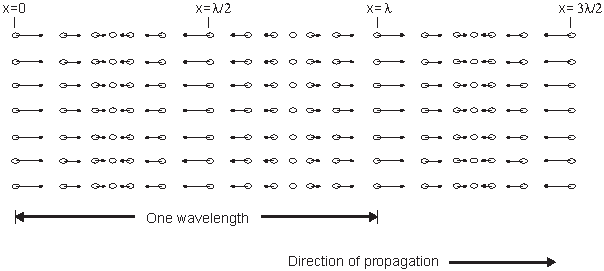
\includegraphics[width=\textwidth]{2_plane_wave_jensen-cropped.pdf}
	\caption[Particle displacement for a propagating ultrasound wave]{Particle displacement for a propagating ultrasound wave \cite{JensenUltrasoundBook}}
	\label{fig:2_planewave_jensen}
\end{figure}
\gls{us} is a technology that transmit sound wave with frequencies above the audible range (\qtyrange[range-units = single]{20}{20e3}{\hertz}) to mechanically vibrate matter. The particles in the medium would be at rest and distributed uniformly before any disturbance. The wave propagates as a disturbance and the particles oscillate around their mean position due to the presence of the ultrasonic wave. Typically the \gls{us} frequency band used in clinical settings are from \qtyrange[range-units = single]{1}{15}{\mega\hertz} \cite{Szabo_UltrasoundBook_2}. \Cref{fig:2_planewave_jensen} visualizes the propagation of a plane wave in matter. The oscillation occurs parallel to the wave's direction, making it longitudinal, and the disturbance will propagate with the variable $c$, which is determined by the medium and is given by \cref{eq:2_velocity_c}.
\begin{equation} \label{eq:2_velocity_c}
	c = \sqrt{\frac{1}{\rho_{0} \kappa_{S}}}
\end{equation}
Where $\rho_{0}$ is the mean density (\unit{\kilogram\per\meter\cubed}) and $\kappa_{S}$ is the \gls{adiabatic} compressibility (\unit{\meter\squared\per\newton}). Since in the majority of cases, the propagation of ultrasound is linear, it is assumed in this work. The acoustic pressure of the harmonic plane wave is expressed by \cref{eq:2_acoustic_pressure}
\begin{equation} \label{eq:2_acoustic_pressure}
	p(t,z)=p_{0} e^{j(\omega t - k z)}
\end{equation}
And propagates along the $z$-axis. $\omega$ is the angular frequency, $k$ is the wave number and is expressed by $k=\nicefrac{\omega}{c}=\nicefrac{2\pi}{\lambda}$, and $_{0}$ is the acoustic pressure amplitude. A spherical wave is expressed by \cref{eq:2_spherical_wave}
\begin{equation} \label{eq:2_spherical_wave}
	p(t,r)=p_{0} e^{j(\omega t - k r)}
\end{equation}
Where $r$ is radial distance, and is defined in a polar coordinate system. For each time instance, the acoustic pressure $p(t,r)$ is constant over a fixed radial position. In this scenario, the pressure amplitude is given by $p_{0}(r) = \nicefrac{k_{p}}{r}$, where $k_{p}$ is a constant since the energy of the outgoing wave must be constant.  Particle speed $u$ is dependent on the pressure caused by a wave expressed by \cref{eq:2_particle_speed}
\begin{equation} \label{eq:2_particle_speed}
	u = \frac{p}{Z}
\end{equation}
Where $Z$ is the characteristic acoustic impedance, defined as the ratio of acoustic pressure to particle speed at a given position in the medium and is expressed by \cref{eq:2_acoustic_impedance}.
\begin{equation} \label{eq:2_acoustic_impedance}
	Z = \rho_{0} c
\end{equation}

Characteristic acoustic impedance $Z$ is one of the most significant variables in the characterization of propagating plane waves. Reference values for density, speed of sound, and characteristic acoustic impedance can be seen in \cref{tab:2_density_tissue}.

\begin{table}[ht]
	\centering
	\caption[Approximate density, sound speed, and acoustic impedance of human tissue types]{Approximate density, sound speed, and acoustic impedance of human tissue types \cite{JensenUltrasoundBook}}
	\label{tab:2_density_tissue}
	\sisetup{range-phrase=--,range-exponents = combine}
	\begin{tblr}[]{ 
		colspec = {XSSS},
		row{1} = {guard,m,font=\small\bfseries},
		}
		\toprule
		Medium & {Density ($\rho_{0}$)\\\unit[per-mode = symbol]{\kilogram\per\meter\cubed}} & {Speed of sound ($c$)\\\unit[per-mode = symbol]{\meter\per\second}} & {\textbf{Acoustic impedance ($Z$)}\\\unit[per-mode = symbol]{\kilogram\per\meter\squared\per\second}} \\ \midrule
		Air             & 1.2     & 333            & 0.4e3       \\
		Blood           & 1.06e3    &    1566        &  1.66e6     \\
		Bone            & \numrange{1.38e3}{1.81e3}  &   \numrange{2070}{5350}       & \numrange{3.75e6}{7.38e6} \\
		Brain           &  1.03e3       & \numrange{1505}{1612}  & \numrange{1.55e6}{1.66e6} \\
		Fat             &  0.92e3  &  1446 & 1.33e6 \\
		Kidney          &  1.04e3  & 1567 & 1.62e6 \\
		Lung            &  0.4e3  &  650  & 0.26e6 \\
		Liver           &  1.06e3  &  1566  & 1.66e6 \\
		Muscle          &  1.07e3  & \numrange{1542}{1626} & \numrange{1.65e6}{1.74e6} \\
		Spleen          &  1.06e3  & 1566 & 1.66e6 \\
		DI				&  1e3  & 1480 & 1.48e6 \\ \bottomrule
	\end{tblr}
\end{table}

In the following sections, various acoustic wave phenomena will be briefly described.

\subsection{Scattering}
A wave propagating through a medium continues in the same direction until it encounters a new medium. When this occurs, a portion of the wave is transmitted into the new medium with a change in direction. Because the scattered wave is the result of several contributors, it is necessary to define it statistically. The amplitude distribution is Gaussian \cite{JensenUltrasoundBook} and can thus be fully described by its mean and variance. The mean value is zero because the dispersed signal is caused by variances in the acoustic characteristics in the tissue. The correlation between multiple data is what allows ultrasound to determine blood velocities. Because minor movements have a significant correlation, it is feasible to discover alterations in location by comparing sequential measurements of moving structures, such as blood cells. In medical ultrasound, only one transducer is used to transmit and receive, and only the backscattered signal is analysed. The power of the scattered signal is defined by the scattering cross-section, which in small cases means a uniform intensity $I_{i}$, and is expressed by \cref{eq:2_scatter_power}.
\begin{equation} \label{eq:2_scatter_power}
	P_{s} = I_{i} \sigma_{s c}
\end{equation}
Where $\sigma_{s c}$ is the scattering cross-section in square meters. The backscattering cross section is material dependant and determines the intensity of the scattering. If the dispersed energy is evenly emitted in all directions, the scattered intensity is given by \cref {eq:2_scatter_intensity}.
\begin{equation} \label{eq:2_scatter_intensity}
	I_{s} = \frac{P_{s}}{4 \pi R^{2}} = \frac{\sigma_{sc}}{4 \pi R^{2}} \cdot I_{i}
\end{equation}
Where $R$ is distance to the scattering region \cite{JensenUltrasoundBook}. This results in a spherical wave. A transducer with radius $r$ gives the power $P_{r}$, presuming the attenuation and focus is neglected, and is expressed by \cref{eq:2_transducer_r_power}.
\begin{equation} \label{eq:2_transducer_r_power}
	P_{r} = I_{s} \pi r^{2} = \sigma_{s c} \frac{r^{2}}{4 R^{2}} \cdot I_{i}
\end{equation}

The backscattering coefficient, which characterizes scattering from a volume of scatterers, is another measure of scattering strength. It is defined as the average received power per steradian volume of scatterers when flooded with plane waves of unit amplitude and the unit is \unit{1\per\centi\meter\steradian}. Backscattering coefficients in the blood are significantly lower than the backscattering coefficients from various tissue types. This poses a challenge when estimating blood flow close to tissue vessel walls \cite{ShungScattering1992,JensenUltrasoundBook}.

\subsection{Attenuation}
The ultrasonic wave will be reduced as it propagates through the tissue due to absorption and scattering. The attenuation in tissue is frequency dependent, with greater attenuation with increasing frequency. Because of absorption and dispersion, the ultrasonic wave will be attenuated as it travels through the tissue. The relationship between attenuation, distance travelled, and frequency is often linear. Attenuation in the tissue occurs as a result of both dispersion, which spreads energy in all directions, and absorption, which turns it into thermal energy. 

\begin{table}[ht]
	\centering
	\caption[Approximate attenuation values for human tissue]{Approximate attenuation values for human tissue
		\cite{JensenUltrasoundBook}}
	\label{tab:my_label}
	\sisetup{range-phrase=--,range-exponents = combine}
	\begin{tblr}[]{%
			colspec = {lS},
			row{1} = {guard, m, font=\small\bfseries},
		}
		\toprule
		Tissue & {Attenuation \\ $\unit[per-mode = symbol,inter-unit-product =\cdot]{\dB\per\mega\hertz\per\centi\meter}$ } \\ 
		\midrule
		Liver & \numrange{0.6}{0.9}{} \\
		Kidney & \numrange{0.8}{1}{} \\
		Spleen & \numrange{0.5}{1}{}\\
		Fat & \numrange{1}{2}{} \\
		Blood & \numrange{0.17}{0.24}{} \\
		Plasma & 0.01 \\
		Bone & \numrange{16}{23}{} \\
		\bottomrule
	\end{tblr}
\end{table}

The pressure of a wave propagating in $z$-direction decreases exponentially expressed by \cref{eq:2_attenuation_pressure}
\begin{equation} \label{eq:2_attenuation_pressure}
	p(z) = p(z=0) e^{-\alpha z}
\end{equation}
Where $p(z=0)$ is the pressure in the point of origin and $\alpha$ is the attenuation coefficient. The attenuation coefficient unit is \si{\neper\per\centi\meter} and, alternatively, \si{\dB\per\centi\meter} with the relationship described in \cref{eq:2_attenuation_coefficient}. 

\begin{subequations} \label{eq:2_attenuation_coefficient}
	\begin{align}
		\ensuremath{\alpha &= \frac{1}{z} \ln \frac{p(z=0)}{p(z)} \\
		\alpha( \si{\dB\per\centi\meter} ) &= 20 ( log_{10}e) \alpha ( \si{\neper\per\centi\meter}) = 8.68\alpha (\si{\neper\per\centi\meter})}
	\end{align}
\end{subequations}

The significance of absorption and scattering in ultrasonic attenuation in biological tissues is a point of contention. Scattering adds just a few per cent to attenuation in most soft tissues. As a result, it is fair to conclude that absorption is the primary mechanism of ultrasonic attenuation in biological tissues \cite{ShungUltrasound_Book}.

\subsection{Transducer}

\begin{figure}[ht]
	\centering
	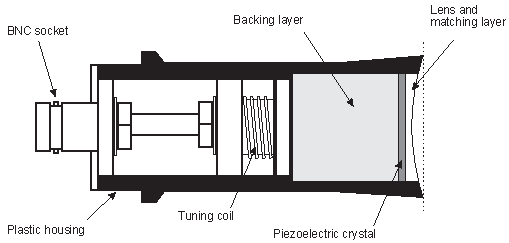
\includegraphics[width=.6\textwidth]{2_transducer_construction-cropped.pdf}
	\caption[Single element ultrasound transducer construction]{Single element ultrasound transducer construction \cite{JensenUltrasoundBook}}
	\label{fig:2_transducer_construction}
\end{figure}

A layperson knows transducers as speakers and microphones in the context of PA systems. In the case of medical \gls{us} it is the device that generates the acoustic pressure field, which is emitted into the tissue. The transducer has a piezoelectric crystal inside the housing. When excited, this crystal emits ultrasound waves toward flowing blood. The red blood cells will reflect a fraction of the emitted waves. These reflected waves are of a different frequency than the transmitted wave. If the red blood cells move away from the transducer, the frequency will be lower. If the red blood cells are moving towards the transducer, the frequency will be higher. This is caused by the \gls{doppler}. The reflected ultrasonic waves return to the crystal and are converted back into electrical signals. The single-element transducer shown in \cref{fig:2_transducer_construction} has a minimal imaging window and has to be mechanically manipulated to obtain a wide window, which is unfeasible for responsive high-frequency imaging. Thus, usually an array transducer is used. Various types of \gls{us} transducer exist with different strengths and weaknesses, shown in \cref{fig:2_transducer_types}. 

\begin{figure}[ht]
	\centering
	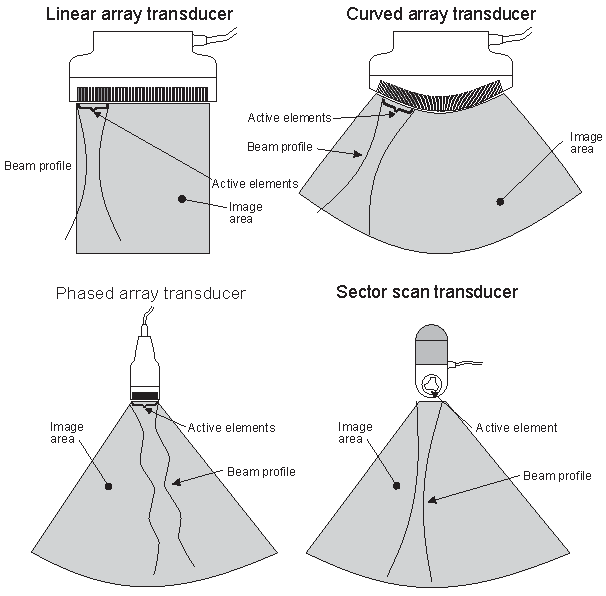
\includegraphics[width=.8\textwidth]{2_transducer_types-cropped.pdf}
	\caption[Transducer types for acquiring B-mode images]{Transducer types for acquiring B-mode images \cite{JensenUltrasoundBook}}
	\label{fig:2_transducer_types}
\end{figure}

\subsection{Doppler effect} \label{sec:doppler_effect}

\begin{figure}[ht]
	\centering
	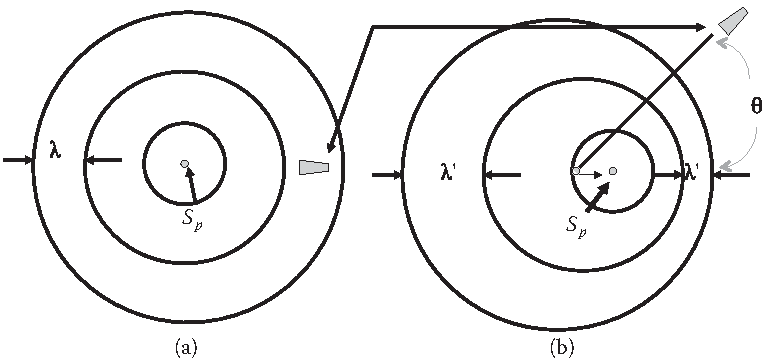
\includegraphics[width=.8\textwidth]{2_doppler_shung-cropped.pdf}
	\caption[Doppler effect diagram]{Doppler effect diagram. A stationary observer perceives a change in frequency of a wave generated by a moving source toward the observer as a result of a wavelength shift from $\lambda\ $ to $\lambda^{\prime}$. In (a), the source is still. In (b), the source is moving at a velocity $v$. \cite{ShungUltrasound_Book}}
	\label{fig:2_doppler_effect}
\end{figure}

The Doppler effect is a phenomena in which an observer perceives a shift in the frequency of sound emitted from a source when either the source or the observer is moving, or both are moving. The reason for the perceived change in frequency is visualised in \cref{fig:2_doppler_effect}. In diagram (a), the source $S_{p}$ is stationary and producing a spherical distribution pattern of the wave with the perceived frequency of the observer is given by $f=\nicefrac{c}{\lambda}$, where $c$ is the velocity of the wave in the medium and $\lambda$ is the wavelength. In diagram (b), the sound source is moving towards the right with a velocity $v$. The locomotion of the source changes the distribution pattern and causes a longer wavelength on the left, indicating a lower perceived frequency, and a shorter wavelength on the right, indicating a higher perceived frequency, both denoted as $\lambda^{\prime}$ in the diagram. In the case of the observer on the right side, the perceived frequency becomes \cref{eq:2_doppler_effect}.

\begin{equation} \label{eq:2_doppler_effect}
	f^{\prime} = \frac{c}{\lambda} = \frac{c}{\lambda - v T} = \frac{c}{(c-v)T} = \frac{c}{c-v}\cdot f_{0}
\end{equation}
And viceversa, on the left side, the perceived frequency becomes \cref{eq:2_doppler_effect2}.
\begin{equation} \label{eq:2_doppler_effect2}
	f^{\prime} = \frac{c}{c+v} \cdot f_{0}
\end{equation}
Where \todo{Hvad mangler her?}

This perceived difference between the frequency that is transmitted from the source $f_{0}$, and the perceived frequency $f^{\prime}$ is also called the Doppler frequency, $f_{d}$. When these connections are combined, the Doppler frequency for a source moving with velocity $v$ and an observer travelling with velocity $v^{\prime}$ is given by \cref{eq:2_doppler_moving}.
\begin{equation} \label{eq:2_doppler_moving}
	f_{d} = f^{\prime} - f = \left( \frac{c + v^{\prime}}{c - v}-1 \right)
\end{equation}
If both source and observer are moving with the same velocity, $v$, assuming $c\gg v$, the $v$ cancels out and the expression is reduced to \cref{eq:2_doppler_reduced}.
\begin{equation} \label{eq:2_doppler_reduced}
	f_{d} = \frac{2 v f}{c}
\end{equation}

If the velocity of the moving source is traveling with an incident angle $\theta$, the $v$ in \cref{eq:2_doppler_reduced} is replaced with $v (\cos\theta)$. This results in the expression found in \cref{eq:2_doppler_theta} and forms the basis for applied \gls{doppler} measurements.
\begin{equation} \label{eq:2_doppler_theta}
	f_{d} = \frac{2 v(\cos\theta) f}{c}
\end{equation}

The Doppler effect is used in ultrasonic Doppler devices used to image blood flow \gls{transcutaneous}ly. An ultrasonic transducer in these devices sends ultrasonic waves into a blood artery, and the scattered radiation from moving red cells is measured by either the same transducer or a second transducer. The Doppler frequency, which is determined by the velocity of red blood cells, is extracted using modern electronic demodulation techniques.

\section{Flow Physics}
\begin{figure}[ht!]
	\centering
	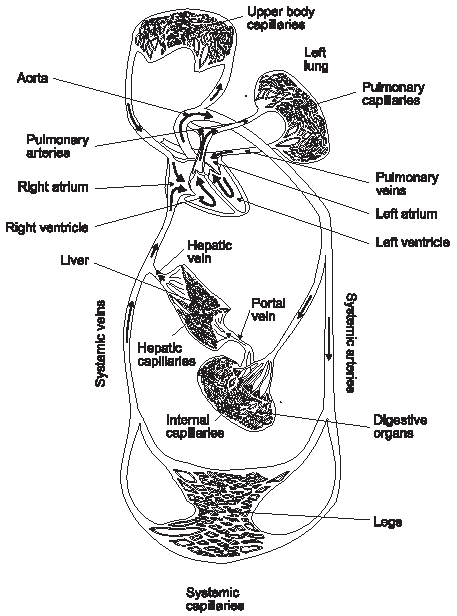
\includegraphics[width=\textwidth]{2_flow_circulatory_system_cropped.pdf}
	\caption[Circulatory system of the human body]{Circulatory system of the human body \cite{JensenUltrasoundBook}}
	\label{fig:2_circulatory_system}
\end{figure}

The flow physics of the human circulatory system are sophisticated, and numerous nonstationary flow patterns emerge. The human circulatory system takes care of transporting oxygen and nutrients to organs, as well as disposing of waste products produced by metabolism. It is possible because the blood within the circulatory system contains several smaller subcomponents, such as plasma and formed cellular elements that perform these vital functions. Initially, blood is discharged from the left ventricle of the heart through the aorta and travels to all areas of the body through multiple branches of the arterial tree. When blood flows through the arteries, it enters smaller channels known as arterioles. These arterioles lead to a network of tiny capillaries through which nutrients and waste materials are exchanged between the blood and the organs. The capillaries connect to form a network of venulae, which supply the veins and deliver blood back to the heart. This system, in its entirety, is called systemic circulation. A diagram of the circulatory system as described above can be seen in \cref{fig:2_circulatory_system}. In summary, when examining the elements that comprise the circulatory system, it consists of several components:
\begin{itemize}
	\item Heart, the primary organ of the circulatory system that maintains blood pressure and controls blood velocity.
	\item Blood, and its sub-components
	\begin{itemize}
		\item Plasma, which forms the primary volume and contains nutrients and formed cellular elements.
		\item Red and white blood cells, which carry oxygen and fight off infections, respectively.
		\item Platelets, which are also known as thrombocytes, have the function of clotting during blood vessel injury.
	\end{itemize}
	\item Blood vessels
	\begin{itemize}
		\item Arteries (and arterioles), transport oxygenised blood to organs and tissues at high pressure and velocity.
		\item Capillaries are thin but wide-ranging blood vessels that perform the exchange of matter between the circulatory system and tissue.
		\item Veins (and venules) carry blood back to the heart at low pressure and velocity.
	\end{itemize}
\end{itemize}

\subsection{Blood flow}
Blood flow is the amount of blood that goes through a blood vessel in a particular period of time, and has a complicated flow pattern due to its pulsing flow. Advanced analysis of haemodynamics is not within the scope of this report, so the explanation will be brief. The primary forces that determine the blood flow $F$ are the pressure difference across a blood vessel and vascular resistance. It is determined by Ohm's law as in \cref{eq:2_flow_ohms_law}.
\begin{equation} \label{eq:2_flow_ohms_law}
	F = \frac{\Delta P}{R}
\end{equation}
Where $\Delta P$ is the pressure difference across the blood vessel and $R$ is the vascular resistance. The pressure difference $\Delta P$ is calculated with \cref{eq:2_pressure_diff}.
\begin{equation} \label{eq:2_pressure_diff}
	\Delta P = P_{1}-P_{2}
\end{equation}
Where $P_{1}$ and $P_{2}$ are the blood pressures measured at each end of the blood vessel. Pressure has a significant importance on blood flow because an increase in arterial pressure not only increases the force that pushes blood through the capillaries but also expands the vessels, lowering vascular resistance.

\section{Devices}
\begin{figure}[ht]
	\centering
	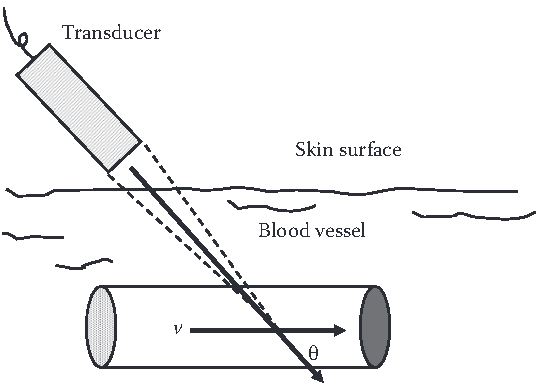
\includegraphics[width=.6\textwidth]{2_ultrasound_scan.pdf}
	\caption[Diagram of ultrasound wave transmitted and reaching blood vessel with incident angle $\theta$]{Diagram of \gls{us} wave transmitted and reaching blood vessel with incident angle $\theta$ \cite{ShungUltrasound_Book}}
	\label{fig:2_ultrasound_flow_scan}
\end{figure}

A device that measures the flowing of blood is called a flowmeter. Flowmeters may be used both inside and outside of vessels. One of the flowmeters that may be used outside the vessel to monitor flow is \gls{us}. \Cref{fig:2_ultrasound_flow_scan} depicts an ultrasonic wave of frequency $f$ insonifying a blood artery, resulting in an angle of $\theta$ relative to velocity $v$. For simplicity, it is assumed that blood flows in a vessel at a constant velocity $v$. The echoes returned are shifted in frequency as described in \cref{eq:2_doppler_theta} earlier in the chapter. The echoes scattered by blood after being insonified by an ultrasonic wave convey information about the velocity of blood flow. Blood flow measurements are often used in clinical settings to determine the status of blood vessels and organ functioning. The two commonly used fundamental techniques for ultrasound Doppler flow measurements are \gls{cw} and \gls{pw}. Both will be explained.

\subsection{Continuous-wave Flowmeter}
\begin{figure}[ht]
	\centering
	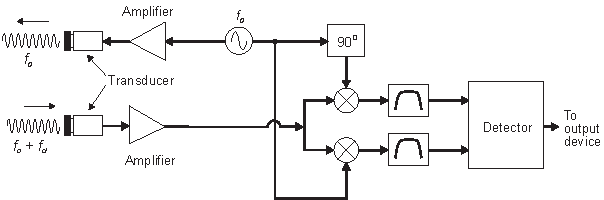
\includegraphics[width=\textwidth]{2_blockdiagram_cwdoppler.pdf}
	\caption[Block diagram of continuous-wave flowmeter]{Block diagram of \gls{cw} flowmeter \cite{JensenUltrasoundBook}}
	\label{fig:2_devices_cw}
\end{figure}
The earliest non-invasive cardiovascular diagnostic technologies relied heavily on \gls{cw} Doppler flowmeters. One of the earliest concepts for a device to estimate and study blood flow was proposed by \citeauthor{Satomura_CW}\cite{Satomura_CW} during the 1950s in Japan. To continuously transmit waves and receive signals from moving reflectors, the \gls{cw} flowmeter uses two transducers. \gls{cw} flowmeters use less sophisticated electronics than \gls{pw} flowmeters. A drawback to the \gls{cw} flowmeter is the lacking depth discrimination due to the continuous characteristic of this device type. A block diagram of a typical \gls{cw} flowmeter can be seen in \cref{fig:2_devices_cw}. The basic principles of the device are previously explained in \cref{sec:doppler_effect}, and the measurement of the device is described in \cref{eq:2_doppler_effect}. The device continuously emits an ultrasonic wave in the first transducer expressed as a function of time by \cref{eq:2_cw_tx} \cite{JensenUltrasoundBook}.
\begin{equation} \label{eq:2_cw_tx}
	e(t) = \cos (2\pi f_{0} t)
\end{equation}
While receiving the backscattered signal on the second transducer expressed by \cref{eq:2_cw_rx} \cite{JensenUltrasoundBook}.
\begin{align} \label{eq:2_cw_rx}
	r_{s}(t) &= a \cos \left( 2\pi f_{0} \alpha (t-t_{0}) \right) \\
	\alpha &\approx 1 - \frac{2 v_{z}}{c} \\
	\alpha t_{0} &\approx \frac{2 d_{0}}{c}
\end{align}
Where $v_{z}$ indicates the velocity in the $z$ direction. Applying the Fourier transform, the expression yields \cref{eq:2_cw_fourier}.
\begin{equation} \label{eq:2_cw_fourier}
	r_{s}(t)\cdot e^{j2\pi f_{0} t} \Longleftrightarrow R_{s}(f-f_{0})
\end{equation}
Where $R_{s}(f-f_{0})$ is the Fourier transform of $r_{s}(t)$. The received signal is then multiplied with a quadrature signal of frequency $f_{0}$ to find the Doppler frequency in \cref{eq:2_cw_quadrature}.
\begin{align} \label{eq:2_cw_quadrature}
	m(t) &= a \left[ \cos(2\pi f_{0} t) + j\sin (2\pi f_{0} t) \right] \cos (2\pi f_{0} \alpha (t-t_{0})) \\
	&= \frac{a}{2} \Bigl\{ \cos (2\pi f_{0} [ (1-\alpha) t- \alpha t_{0} ]) + \cos (2\pi f_{0} [ (1-\alpha) t- \alpha t_{0} ]) \\
	&\quad + j \sin (2\pi f_{0} [ (1-\alpha) t- \alpha t_{0} ]) + j \sin (2\pi f_{0} [(1-\alpha) t- \alpha t_{0} ]) \Bigr\} \nonumber
\end{align}

As is general for quadrature demodulation, the resulting signal contains the frequency components of the sum and difference of the emitted and received signals' frequencies shown in \cref{fig:2_demod_fd_frequency_domain}, where the signals are shown in time and frequency domains. 

\begin{figure}[ht]
	\centering
	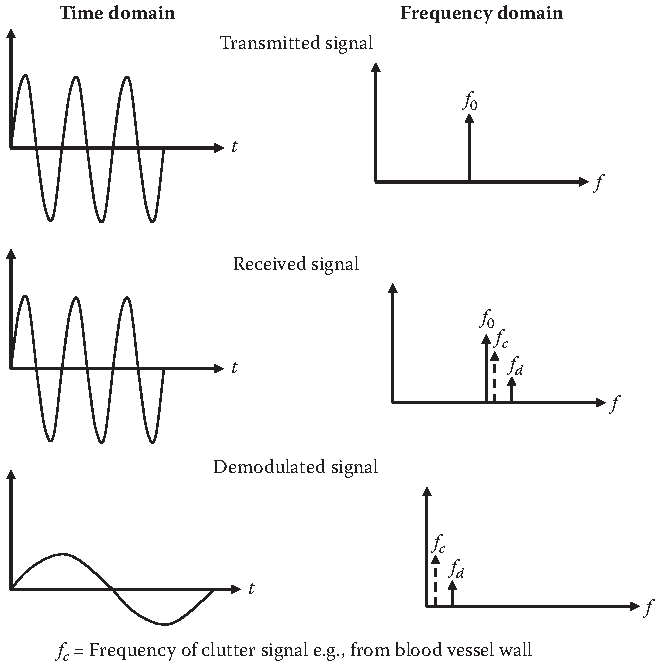
\includegraphics[width=.8\textwidth]{2_demod_fd_frequency_domain-cropped.pdf}
	\caption[Doppler signals in time and frequency domain showing demodulation effects]{Doppler signals in time and frequency domain showing demodulation effects \cite{ShungUltrasound_Book}}
	\label{fig:2_demod_fd_frequency_domain}
\end{figure}

Generally, a \gls{bp} filter is used on the demodulated signal to remove the high-frequency summed signal at twice the frequency of $f_{0}$. The filtered signal after the \gls{bp} filter is expressed by \cref{eq:2_cw_bp} and contains the Doppler shift of the emitted signal.
\begin{equation} \label{eq:2_cw_bp}
	m_{f}(t) \approx \frac{a}{2} e^{\left(j2\pi f_{0} \frac{2v_{z}}{c}t\right)} e^{\left( -j2\pi f_{0} \alpha t_{0} \right)}
\end{equation}
Where the second exponential term is the delay proportional to the time between transmission and receiving of the signal. The selected cutoff frequency is chosen to be much lower than the carrier frequency to remove the carrier wave. One issue with ultrasonic Doppler blood flow monitoring is that the blood vessels that generate large reflected echoes are also moving with a low velocity. These big, slow-moving echoes are referred to as clutter signals in Doppler nomenclature. The band pass filter's low-end cutoff frequency must be designed to minimize interference from these clutter signals. The design of this band pass filter in the low-frequency region, which serves the function of high pass, also known as a clutter rejection filter, has proven troublesome since the magnitude of clutter signals is many orders greater than that of blood and may obfuscate those from slow-moving blood. 

\begin{table}[ht]
	\centering
	\caption[Measured frequency shifts with a Doppler \qty{3}{\mega\hertz} transducer at various velocities at a \qty{45}{\degree} incident angle]{Measured frequency shifts with a Doppler \qty{3}{\mega\hertz} transducer at various velocities at a \qty{45}{\degree} incident angle \cite{JensenUltrasoundBook}}
	\label{tab:2_cw_frequency_shifts}
	\begin{tblr}[]{%
			colspec = {SS},
			row{1} = {guard, m, font=\small\bfseries},
			%vlines, hlines,
		}
		\toprule
		{Velocity $\left(v\right)$ \\ \unit[per-mode = symbol]{\meter\per\second}} & {Doppler frequency $\left(f_{d}\right)$ \\ \unit{\hertz} } \\ 
		\midrule
		0.01 & 28 \\
		0.1 & 276 \\
		0.5 & 1377 \\
		1 & 2755 \\
		2 & 5510 \\
		5 & 13770 \\
		\bottomrule
	\end{tblr}
\end{table}

Seen in \cref{tab:2_cw_frequency_shifts} is an example of measured Doppler frequencies using a \qty{3}{\mega\hertz} transducer using the method shown in \cref{fig:2_ultrasound_flow_scan}. Note that the measured frequencies are all within the audible range.

\subsection{Pulsed-wave Flowmeter}
\begin{figure}[ht]
	\centering
	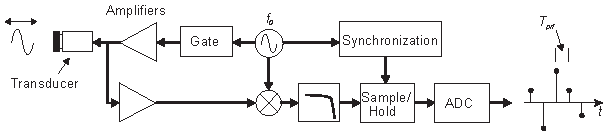
\includegraphics[width=\textwidth]{2_blockdiagram_pwdoppler.pdf}
	\caption[Block diagram of pulsed-wave flowmeter]{Block diagram of \gls{pw} flowmeter \cite{JensenUltrasoundBook}}
	\label{fig:2_devices_pw}
\end{figure}
The concept of a pulsed-wave flowmeter was proposed in \cite{Baker1970} and other related articles. This type of flowmeter is periodically changing from a transmitter to a receiver. In the transmit mode, the transducer emits a series of pulses. When in the receiving mode, the transducer is listening for the backscattered signal. A simplified block diagram can be seen in \cref{fig:2_devices_pw}. The movement of particles within the blood causes a displacement in the backscattered signal. These systems are commonly referred to as \enquote{Doppler systems} even though it is somewhat misleading. The effects of attenuation are also causing a shift in frequency of a higher magnitude than the velocity of particles in the blood. This is because the conventional Doppler effect is not the straightforward methodology that is applied to the analysis of the back-scattered signal. It is, in fact, an artefact. It is the shift in the location of the scatters that is observed, not the shift in the transmitted frequency. \Cref{fig:2_pw_sampling_displacement} shows the received signal after demodulation and filtering; the depth in tissue is fixed here, and the signals displayed on the left side of the figure are the result of a pulse sequence. Each line represents a single pulse, and each pulse is emitted at a pulse repetition frequency, $f_{\textup{prf}}$. Instead, on the right, the dotted line shows the sampled signal formed by taking into account the amplitude of each pulse after a specified time period.

\begin{figure}[ht]
	\centering
	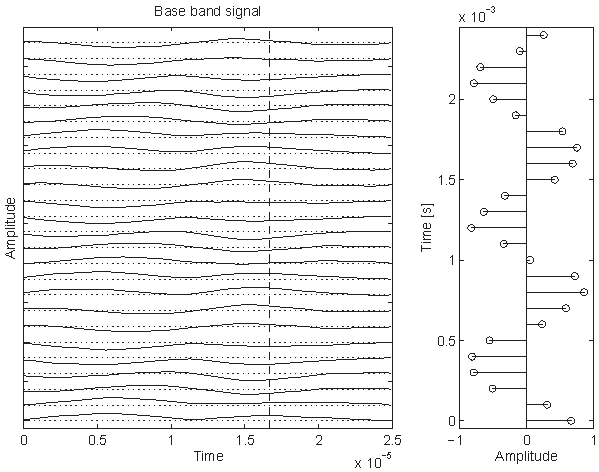
\includegraphics[width=.8\textwidth]{2_pw_pulse_sampling_displacement.pdf}
	\caption[Sampling for a gate pulsed wave system with a single range]{Sampling for a gate pulsed wave system with a single range. To depict the signals on the graph, a single pulse is emitted for each line, and the signals are displaced in amplitude. The sampled signal is displayed on the right. \cite{JensenUltrasoundBook}}
	\label{fig:2_pw_sampling_displacement}
\end{figure}


After the back-scattered signal is received it is multiplied by the centre frequency of the emitted pulse and filtered to remove the sum frequency \cite{JensenUltrasoundBook}. A \gls{adc} quantifies the signal for further signal processing. Referring to displacement \cref{fig:2_pw_sampling_displacement} again, the dashed vertical line represents the sample of each pulse that is taken. If sampling is done $T_{s}$ after pulse emission, the measurement depth is expressed by \cref{eq:2_pw_depth}.
\begin{equation} \label{eq:2_pw_depth}
	d_{0} = \frac{T_{s}c}{2}
\end{equation}
Hypothetically, if the velocity of stationary scatterers in blood was measured, a constant amplitude would be measured. A change in the sample value is observed when there is movement. Between two pulses, the scatterer movement is proportional to the velocity $v_{z}$ in the direction of the ultrasound beam. The time shift of $t_{s}$ is expressed as \cref{eq:2_pw_timeshift}.
\begin{equation} \label{eq:2_pw_timeshift}
	t_{s} = \frac{2v_{z}}{c}\cdot T_{\textup{prf}}
\end{equation}
Where $c$ is the speed of sound, and $T_{\textup{prf}}$ is the timespan between each pulse emission. Taking one sample from each line at a certain depth yields a sampled signal with a frequency proportional to the scatter velocity. Thus, if a sample is taken at the same depth for each line, resulting in a sinusoidal signal proportional in frequency to the scatter velocity \cite{Munk_Thesis} and that signal is expressed by \cref{eq:2_pw_scatter_velocity_a,eq:2_pw_scatter_velocity_b}.
\begin{subequations}
	\begin{align} 
		r(i) &= a(i) \sin \left( 2\pi f_{p} T_{\textup{prf}} \cdot i \right) \label{eq:2_pw_scatter_velocity_a} \\
		f_{p} &= \frac{2 v_{z}}{c} f_{0} \label{eq:2_pw_scatter_velocity_b}
	\end{align}
\end{subequations}
Where $a(i)$ is the amplitude, $f_{0}$ is the emitted frequency, and $\theta$ is the phase factor in the depth of interest. \todo{Hvor er $\theta$ i udtrykket? Omskriv fra Jensen2012} This technique improved the accuracy of the investigations of blood vessels and facilitated the display of velocity profiles. Furthermore, by employing two transducers or a multi-element transducer, duplex mode imaging (displaying both a B-mode picture and a blood velocity estimate) became feasible. Two-transducer systems are no longer utilised since it is easier to create a duplex picture with a multi-element transducer. 

\section{Blood Velocity Estimation}
Once a backscattered signal is received, estimation of velocity can be obtained with multiple methods. In this section the most common methods to estimate blood velocity are mentioned with their strengths and limitations. 
\subsection{Spectral estimation}
\begin{figure}[htbp]
	\centering
	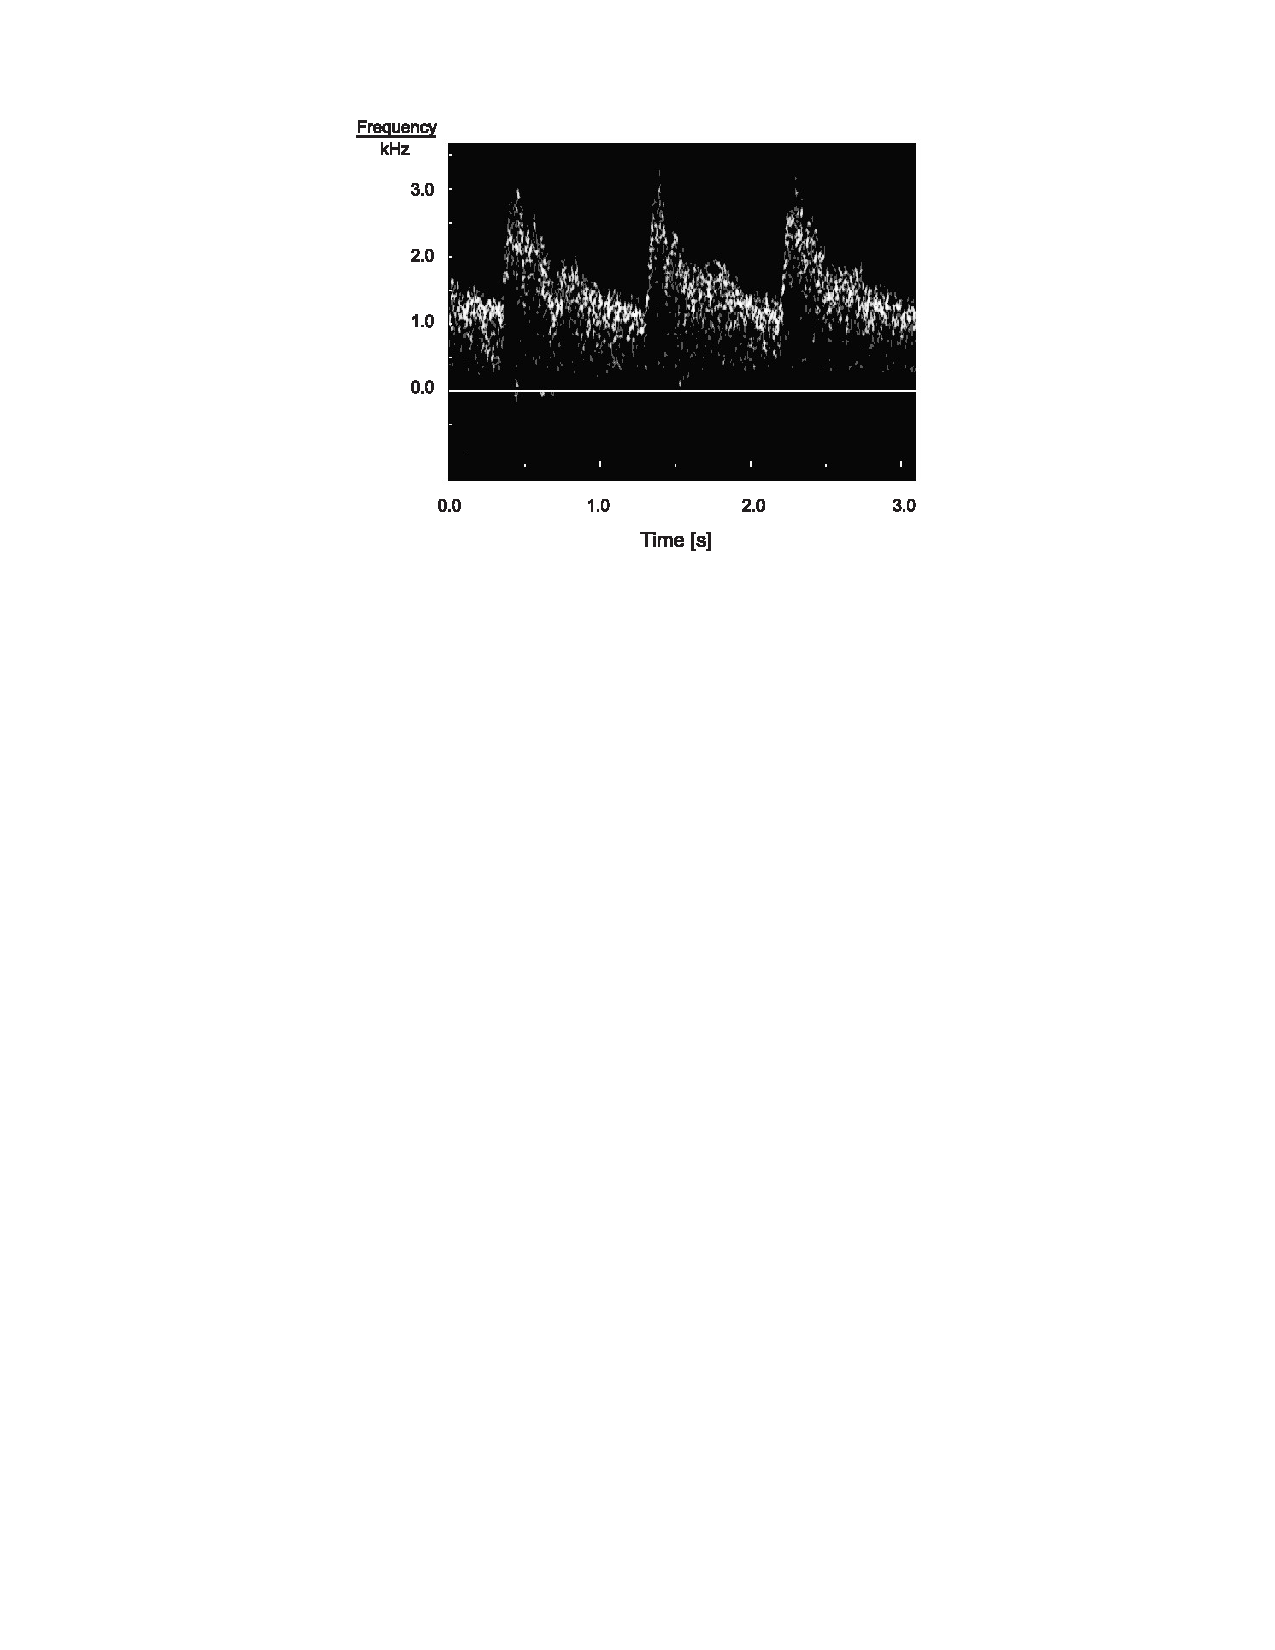
\includegraphics[width=.8\textwidth]{Figures/2_estimation_sonogram_cph.pdf}
	\caption{Arterial sonogram with time-frequency and Doppler shift \cite{JensenUltrasoundBook}}
	\label{fig:2_estimation_sonogram_cph}
\end{figure}

Given that the frequency volume of the received signal is similar to the blood's velocity distribution, the Fourier transform of the received signal can be used to obtain velocity. The spectrogram, usually erroneously known as the Doppler spectrum, can be created by saving the \gls{psd} together. The \gls{psd} is calculated for each of the components that make up the received signal in order to accomplish this. A quadrature demodulated signal is used to display both positive and negative frequencies. When these spectra are shown side by side, the evolution of the velocity distribution can then be seen. The ultrasonography of an artery is displayed in \cref{fig:2_estimation_sonogram_cph}. 
	\chapter{Synthesis} \label{cha:synthesis} %\thispagestyle{main}
\begin{figure}[ht]
	\centering
	\resizebox{\textwidth}{!}{
		%\begin{tikzpicture}
%	[outer sep=0,
%>=latex,
%align=center]
%% Draw nodes
%\node[place]		(human_in)	[draw=none]											{Control\\input};
%\node[place]		(embed)		[inner sep=1mm,rectangle,right=10mm of human_in]	{Control\\system};
%\node[place]		(wave_gen)		[inner sep=1mm,rectangle,right=5mm of embed]			{Pulse\\generator};
%\node[place]		(pwr_stg)	[inner sep=1mm,rectangle,right=5mm of wave_gen]	{Power\\stage};
%\node[place]		(tr_switch)	[inner sep=1mm,rectangle,right=5mm of pwr_stg]	{T/R\\switch};
%\node[place]		(transducer)		[inner sep=1mm,rectangle,right=5mm of tr_switch]	{Transducer};
%\node[place]		(preamp)		[inner sep=1mm,rectangle,below=5mm of tr_switch]	{Preamplifier};
%\node[place]		(bpf)		[inner sep=1mm,rectangle,below=5mm of preamp]	{BPF};
%\node[place]		(demod)		[inner sep=1mm,rectangle,left=10mm of bpf]		{Demodulator};
%\node[place]		(lpf1)		[inner sep=1mm,rectangle,above=5mm of demod]		{LPF 1};
%\node[place]		(lpf2)		[inner sep=1mm,rectangle,below=5mm of demod]		{LPF 2};
%\node[place]		(sha1)		[inner sep=1mm,rectangle,left=5mm of lpf1]		{SHA 1};
%\node[place]		(sha2)		[inner sep=1mm,rectangle,left=15mm of lpf1]		{SHA 2};
%
%% Draw lines between nodes
%\draw [|->] 		(human_in) 		to 		(embed);
%\draw [->]			(embed)			to		(wave_gen);
%\draw [->]			(wave_gen)		to		(pwr_stg);
%\draw [->]			(pwr_stg)		to		(tr_switch);
%\draw [<->]			(tr_switch)		to		(transducer);
%\draw [->]			(tr_switch)		to		(preamp);
%\draw [->]			(preamp)		to		(bpf);
%\draw [->]			(bpf)		to		(demod);
%\draw [->]			(demod)		to		(lpf1);
%\draw [->]			(demod)		to		(lpf2);
%\draw [-|>]			(lpf1)		to		(sha1);
%\draw [-|>]			(lpf2)		to		(sha2);
%\draw [-|>]			(sha1)		to		(embed);
%\draw [-|>]			(sha2)		to		(embed);
%
%% Draw rectangle
%\draw[draw=black,dashed,red] (13mm,8mm) rectangle ++(45mm,-15mm);
%\end{tikzpicture}
%\begin{tikzpicture}
%	[outer sep=0,
%	>=latex,
%	align=center,
%	line width = 1pt,
%	% on grid,
%	start chain = going right,
%	node distance = 5cm,
%	%box/.style = {draw, rectangle, font=\huge, on chain},
%	box/.style = {draw, rectangle, on chain},
%	%L/.style = {draw, red, -{Stealth[scale=3,length=3,width=2]}},
%	L/.style = {draw, -{Stealth[scale=3,length=3,width=2]}},
%	%T/.style = {draw, red, rounded corners,
%		T/.style = {draw, rounded corners,
%			to path={-| (\tikztotarget)},
%			-{Stealth[scale=3,length=3,width=2]}}]
%
%		% Draw nodes
%		\node[place]		(human_in)	[draw=none]											{Control\\input};
%		\node[place]		(embed)		[inner sep=1mm,rectangle,right=10mm of human_in]	{Control\\system};
%		\node[place]		(wave_gen)		[inner sep=1mm,rectangle,right=5mm of embed]			{Pulse\\generator};
%		\node[place]		(pwr_stg)	[inner sep=1mm,rectangle,right=5mm of wave_gen]	{Power\\stage};
%		\node[place]		(tr_switch)	[inner sep=1mm,rectangle,right=5mm of pwr_stg]	{T/R\\switch};
%		\node[place]		(transducer)		[inner sep=1mm,rectangle,right=8mm of tr_switch]	{Transducer};
%		\node[place]		(preamp)		[inner sep=1mm,rectangle,below=5mm of tr_switch]	{Preamplifier};
%		\node[place]		(bpf)		[inner sep=1mm,rectangle,below=5mm of preamp]	{BPF};
%		\node[place]		(demod)		[inner sep=1mm,rectangle,left=10mm of bpf]		{Demodulator};
%		\node[place]		(lpf2)		[inner sep=1mm,rectangle,above=5mm of demod]	{LPF 2};
%		\node[place]		(lpf1)		[inner sep=1mm,rectangle,left=5mm of demod]		{LPF 1};
%		\node[place]		(sha2)		[inner sep=1mm,rectangle,left=10mm of lpf2]		{SHA 2};
%		\node[place]		(sha1)		[inner sep=1mm,rectangle,left=27.5mm of lpf2]		{SHA 1};
%
%		% Draw lines between nodes
%		\draw [L,|->] 		(human_in) 		to 		(embed);
%		\draw [L,->]			(embed)			to		(wave_gen);
%		\draw [L,->]			(wave_gen)		to		(pwr_stg);
%		\draw [L,->]			(pwr_stg)		to		(tr_switch);
%		\draw [L,<->]			(tr_switch)		to		(transducer);
%		\draw [L,->]			(tr_switch)		to		(preamp);
%		\draw [L,->]			(preamp)		to		(bpf);
%		\draw [L,->]			(bpf)		to		(demod);
%		\draw [L,->]			(demod)		to		(lpf1);
%		\draw [L,->]			(demod)		to		(lpf2);
%		\draw [T,->]			(lpf1)		to		(sha1);
%		\draw [L,->]			(lpf2)		to		(sha2);
%		\draw [T,->]			(sha1)		to		(embed);
%		\draw [T,->]			(sha2)		to		(embed);
%
%		% Draw rectangle
%		%\draw[draw=black,dashed,red] (13mm,8mm) rectangle ++(45mm,-15mm);
%	\end{tikzpicture}
\begin{tikzpicture}
	[outer sep=0,
	>=latex,
	align=center,
	line width = 1pt,
	% on grid,
	start chain = going right,
	node distance = 5cm,
	%box/.style = {draw, rectangle, font=\huge, on chain},
	box/.style = {draw, rectangle, on chain},
	%L/.style = {draw, red, -{Stealth[scale=3,length=3,width=2]}},
	L/.style = {draw, -{Stealth[scale=3,length=3,width=2]}},
	%T/.style = {draw, red, rounded corners,
		T/.style = {draw, rounded corners,
			to path={-| (\tikztotarget)},
			-{Stealth[scale=3,length=3,width=2]}}]

		% Draw nodes
		\node[place]		(human_in)	[draw=none]											{Control\\input};
		\node[place]		(embed)		[inner sep=1mm,rectangle,right=10mm of human_in]	{Control\\system};
		\node[place]		(wave_gen)		[inner sep=1mm,rectangle,right=5mm of embed]			{Pulse\\generator};
		\node[place]		(pwr_stg)	[inner sep=1mm,rectangle,right=5mm of wave_gen]	{Power\\stage};
		\node[place]		(tr_switch)	[inner sep=1mm,rectangle,right=5mm of pwr_stg]	{T/R\\switch};
		\node[place]		(transducer)		[inner sep=1mm,rectangle,right=10mm of tr_switch]	{Transducer};
		\node[place]		(preamp)		[inner sep=1mm,rectangle,below=5mm of tr_switch]	{Preamplifier};
		\node[place]		(bpf)		[inner sep=1mm,rectangle,below=5mm of preamp]	{BPF};
		\node[place]		(demod)		[inner sep=1mm,rectangle,left=5mm of bpf]		{Demodulator};
		%\node[place]		(lpf2)		[inner sep=1mm,rectangle,above=5mm of demod]	{LPF 2};
		\node[place]		(lpf1)		[inner sep=1mm,rectangle,left=5mm of demod]		{LPF};
		%\node[place]		(sha2)		[inner sep=1mm,rectangle,left=10mm of lpf2]		{SHA 2};
		\node[place]		(sha1)		[inner sep=1mm,rectangle,left=5mm of lpf1]		{SHA};
		\node[place]		(hpf)		[inner sep=1mm,rectangle,above=5mm of sha1]		{HPF};

		% Draw lines between nodes
		\draw [L,|->] 		(human_in) 		to 		(embed);
		\draw [L,->]			(embed)			to		(wave_gen);
		\draw [L,->]			(wave_gen)		to		(pwr_stg);
		\draw [L,->]			(pwr_stg)		to		(tr_switch);
		\draw [L,<->]			(tr_switch)		to		(transducer);
		\draw [L,->]			(tr_switch)		to		(preamp);
		\draw [L,->]			(preamp)		to		(bpf);
		\draw [L,->]			(bpf)		to		(demod);
		\draw [L,->]			(demod)		to		(lpf1);
		%\draw [L,->]			(demod)		to		(lpf2);
		\draw [L,->]			(lpf1)		to		(sha1);
		%\draw [L,->]			(lpf2)		to		(sha2);
		\draw [L,->]			(sha1)		to		(hpf);
		%\draw [T,->]			(sha2)		to		(embed);
		\draw [L,->]			(hpf)		to		(embed);

		% Draw rectangle
		%\draw[draw=black,dashed,red] (13mm,8mm) rectangle ++(45mm,-15mm);
	\end{tikzpicture}
	}
	\caption[Simplified overview of the entire system]{Simplified overview of the entire system}
	\label{fig:1_system_overview}
\end{figure}
A simplified overview of the entire system can be seen in \cref{fig:1_system_overview}. Each of the various modules will be explained during this chapter of the report. Initially, the control system will be briefly explained and the reasons for its design choice. Secondly, the signal chain in the transmitter will be outlined and how the transducer is driven by the power stage with the added protective switching circuit. Finally, the analogue front-end will be further explained with its various subcircuits for filtering, amplifying, demodulating, and sampling the signal. Lastly, the design of the \gls{dsp} within the control system will be explained.

\section{Control System}
\begin{figure}[htbp]
	\centering
	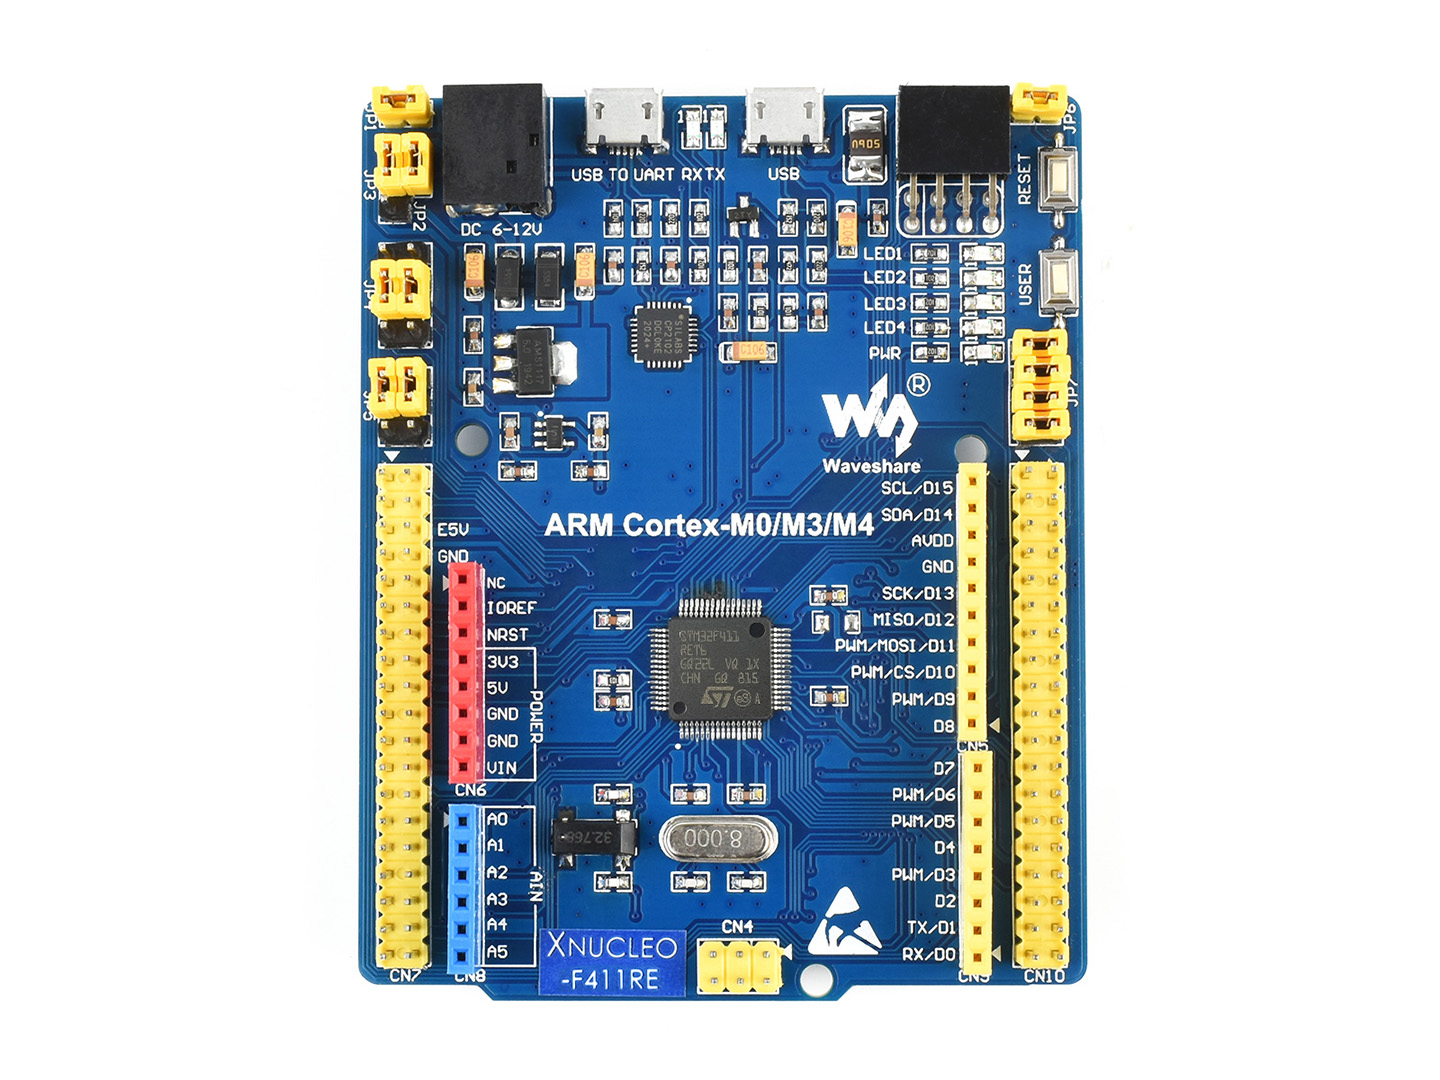
\includegraphics[width=.8\textwidth]{Figures/3_xnucleo_f411re.jpg}
	\caption{XNUCLEO-F411RE development board by Waveshare}
	\label{fig:3_xnucleo_f411re_pcb}
\end{figure}
The choice of platform for controls and data acquisition is an embedded system. A microcontroller is a small computer that is built into a single \gls{ic} chip. It includes a \gls{cpu}, memory, and \gls{io} peripherals, and it is designed to perform a specific set of tasks. Microcontrollers are used in a wide range of electronic devices, including appliances, automobiles, industrial control systems, and consumer electronics. Microcontrollers are often used in applications where a small, low-power device is needed to perform simple tasks, such as controlling a motor or reading a sensor. They are usually programmed in a high-level language, such as C or C++, and they can be programmed to perform a variety of tasks, depending on the specific application. The chosen \gls{mcu} for this project is XNUCLEO-F411RE, visible in \cref{fig:3_xnucleo_f411re_pcb}, because it is sufficient for the application and sourcing limitations within the \gls{ic} supply chain. For implementing the control system, a \gls{rtos} can offer multiple benefits for the embedded system development. A RTOS is an operating system that is designed to handle real-time applications. Real-time applications are those that require timely processing of data in order to function correctly. This can include tasks such as controlling industrial machinery, monitoring and controlling processes. Real-time operating systems are designed to prioritize certain tasks and ensure that they are completed within a specific timeframe. They do this by allocating a certain amount of processing resources to each task, and by interrupting the execution of lower-priority tasks as needed to ensure that high-priority tasks are completed on time. RTOSs typically include features such as preemptive scheduling, real-time communication, and support for multiple processors and hardware architectures. Alternatively, a vendor-locked baremetal implementation is an option, in this case, STM32 HAL. Notable differences between the two approaches are, but not limited to:
\begin{itemize}
	\item Multitasking: RTOS allows for parallel execution that enable more complex applications.
	\item Portability: Standard modules mean that the same code can be easily ported to other devices and even other platforms without modifications.
	\item Reduced development time: Especially for rapid prototype development, using pre-existing APIs significantly reduces development time by providing many of the low-level tasks such as scheduling, resource management, and timing by the operating system.
\end{itemize}

%\subsection{Development Environment}
%\begin{figure}[htbp]
%	\centering
%	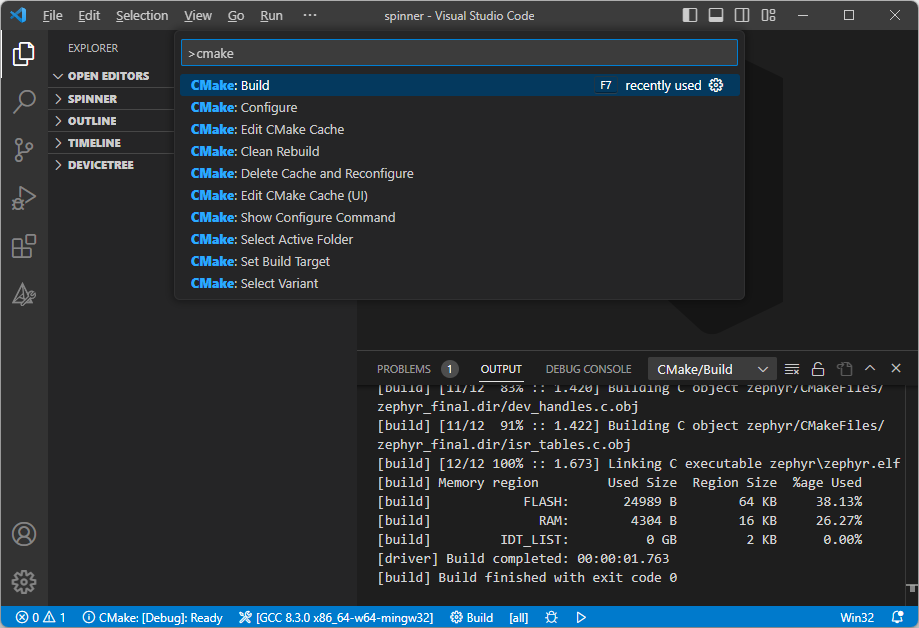
\includegraphics[width=.8\textwidth]{Figures/3_cmake_vscode.png}
%	\caption[VSCode editor with CMake Tools active]{VSCode editor with CMake Tools active, displaying available tasks}
%	\label{fig:3_vscode_cmake_build}
%\end{figure}
%
%Visual Studio Code (VSCode) is an \gls{open-source} code editor developed by Microsoft. It is designed to be highly customizable and efficient, with a wide range of features and extensions that allow developers to customize their workflows and improve their productivity. VSCode works in synergy with CMake through an extension. CMake is a cross-platform build system that helps developers manage the build process for their projects. It is used to generate build files for different platforms and build systems, to build projects on a wide range of platforms. When using CMake with VSCode, the basic idea is to use the CMake extension for VSCode to generate the appropriate build files for the target platform, and then use the VSCode tasks and debugging capabilities to build and debug the project. After setup of VSCode, the CMake Tools \cite{cmake} extension can be found in the VSCode Marketplace. The CMake Tools extension allows you to create, configure and build CMake projects from within VSCode. Once the extension is installed, you can create a new CMake project and configure it by specifying the path to the \texttt{CMakeLists.txt} file and other settings like the target platform and build configuration. After configuring the project, the VSCode tasks are provided to build and run the project. These tasks are defined in the \texttt{tasks.json} file, which can be customized to specify the build command and other options. Examples of tasks are build the project, cleaning the build directory, or running tests. The available CMake tasks are shown in \cref{fig:3_vscode_cmake_build}. In addition to building and running the project, VSCode allows for debugging capabilities to debug code.

\section{Pulse Generator}
Initially, a pulse generator was designed by using a programmable synthesizer circuit, but due to constraints within generating complementary PWM with dead-time when driving the half-bridge, a timer based PWM generation in the microcontroller is preferable. In a half-bridge power stage, dead-time refers to the amount of time that elapses between the moment when one of the switches in the half-bridge (either the high-side or the low-side switch) turns off and the moment when the other switch turns on. During the dead-time, both switches in the half-bridge are off, which means that there is no current flowing through either switch in the half-bridge. A scenario where both switches are on, can cause problems if the output of the half-bridge is connected to a load, as it may cause the load to behave erratically or even be damaged. To avoid these problems, it is important to carefully consider the amount of dead-time in a half-bridge power stage. In general, a longer dead-time will reduce the risk of damage to the load, but it will also reduce the efficiency of the power stage, as energy will be lost during the dead-time. Therefore, it is important to carefully balance the trade-off between efficiency and safety in order to determine the optimal amount of dead-time for a given half-bridge power stage. Based on discussions during design review, it was decided to change approach and generate the two complementary PWM signals by configuring the PWM module of the controller with the functionality though with a trade-off in resolution. However, for this application there is no need to amplitude modulate the output signal.
In the context of a PW Doppler system, it is desired to generate 4 signals:
\begin{itemize}
	\item \qty{5}{\mega\hertz} complementary signal \texttt{PWM} with dead-time for the pulsed burst during transmit mode.
	\item \qty{5}{\mega\hertz} complementary signal \texttt{PWMN} with dead-time and opposite phase from \texttt{PWM}.
	\item \qty{10}{\kilo\hertz} signal \texttt{PRF} for the timing control of the transmit/receive switch.
	\item \qty{20}{\mega\hertz} clock signal \texttt{CLK} for the demodulation circuit in the receiver.
	\item \texttt{PULSE} and \texttt{GATE} controlled by \texttt{PRF} for S/H control with pulse length $t_{\mathrm{pulse}} = N_{\mathrm{pulse}} \times T_{\mathrm{prd}}$, where $T_{\mathrm{prd}} = \sfrac{1}{f_{\mathrm{pwm}}}$. \texttt{GATE} is delayed from pulse by \texttt{sample depth}.
\end{itemize}

\begin{figure}[htbp]
	\centering
	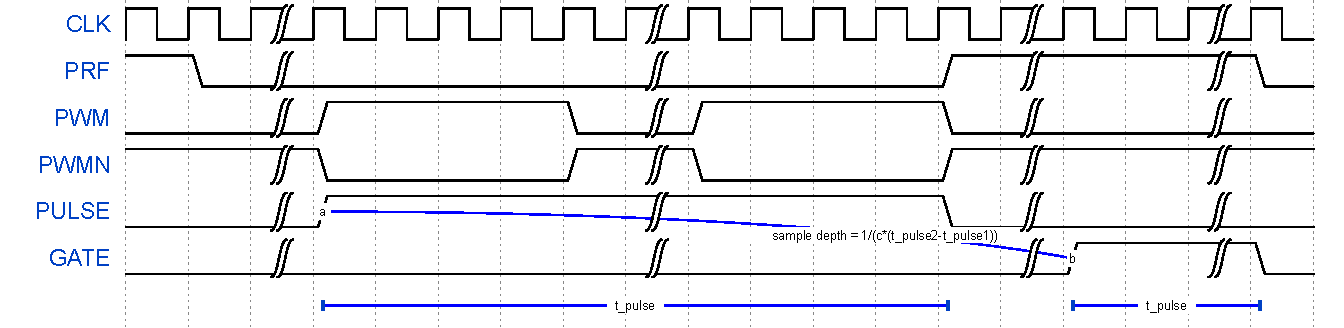
\includegraphics[width=\textwidth]{Figures/3_wavedrom.pdf}
	\caption{Timing diagram of various control signals for an arbitrary $n$ length pulse chain expressed by the second diagram gap}
	\label{fig:3_pulse_timing_diagram}
\end{figure}

\begin{figure}[htbp]
	\centering
	\resizebox{\textwidth}{!}{%
    \begin{tikzpicture}[
	node distance = 20mm and 20mm,
	V/.style = {draw, fill=gray!10},
	G/.style = {draw, fill=white},
	every edge quotes/.style = {auto, font=\footnotesize, sloped}
	]
	\begin{scope}[nodes=V]
		\node (1)   {Transducer};
		\node (2) [below=10mm of 1]    {TR Switch};
		%\node (3) [right=of 2]          {3};
		\node (4) [right=of 2]    {Pulse Generator};
		%\node (5) [below left=of 4]    {5};
		\node (6) [below=of 2]          {Power Stage};
		%\node (7) [right=of 4]          {Control System};
		%\node (8) [right=of 7]          {Inputs};
		\node (9) [above=10mm of 4]      {Demodulator};
		\node (10) [right=of 4]     {Time Delay};
		\node (11) [above=10mm of 10]     {Sample and Hold};
	\end{scope}
	\draw   (1)  edge[""] (2)
	%       (2)  edge["B"] (3)
	%      (3)  edge["C"] (4)
	(4)  edge["PWM/PWMN"] (6)
	(2)  edge["PRF"] (4)
	(6)  edge["HV PULSES"] (2)
	(4)  edge["CLK"]   (9)
	(4)  edge["PULSE"] (10)
	(10) edge["GATE"] (11);
	%
	%       (4)  edge["G"] (7)
	%       (7)  edge["H"] (8);
\end{tikzpicture}
}%
\caption{Block diagram of pulse generator signals and modules}
\label{fig:3_pulsegenerator_signal_block_diagram}
\end{figure}

\section{Power Stage}
%\begin{figure}[htbp]
%	\centering
%	\resizebox{.6\textwidth}{!}{%
%		\begin{circuitikz}
%			\tikzstyle{every node}=[font=\LARGE]
%			\draw (7,12) to[Tnmos] (7,14);
%			\draw (6.15,13) to[short] (6,13);
%			\draw (7,16) to[Tpmos] (7,18);
%			\draw (6.15,17) to[short] (6,17);
%			\draw (5.5,16.5) to[R,l={ \normalsize $R1$}] (5.5,17.75);
%			\draw (5,16.5) to[empty Zener diode,l={ \normalsize $D1$}] (5,17.75);
%			\draw (5,13) to[empty Zener diode,l={ \normalsize $D2$}] (5,11.75);
%			\draw (5.5,13) to[R,l={ \normalsize $R2$}] (5.5,11.75);
%			\draw [](5,17.75) to[short] (7,17.75);
%			\draw [](7,17.75) to[short] (7,17.5);
%			\draw[] (6,16.5) to[short] (5,16.5);
%			\draw[] (6,13) to[short] (5,13);
%			\draw [](7,12) to[short] (7,11.75);
%			\draw[] (7,11.75) to[short] (5,11.75);
%			\draw (5.5,13) to[short, -*] (5.5,13);
%			\draw (5.5,11.75) to[short, -*] (5.5,11.75);
%			\draw (5.5,17.75) to[short, -*] (5.5,17.75);
%			\draw (5.5,16.5) to[short, -*] (5.5,16.5);
%			\draw [ -Stealth] (7,17.75) -- (7,18.25);
%			\draw [ -Stealth] (7,11.75) -- (7,11.25);
%			\draw [](5,16.5) to[short, -o] (4.25,16.5);
%			\draw [](5,13) to[short, -o] (4.25,13);
%			\draw (7,15.5) to[D,l={ \normalsize $D3$}] (8.25,15.5);
%			\draw (8.25,14) to[D,l={ \normalsize $D4$}] (7,14);
%			\draw [](8.25,14.75) to[short, -o] (9.25,14.75);
%			\draw [](8.25,14) to[short] (8.25,15.5);
%			\draw (8.25,14.75) to[short, -*] (8.25,14.75);
%		\end{circuitikz}
%	}%
%
%	\label{fig:my_label}
%\end{figure}
\begin{figure}[htbp]
	\centering
	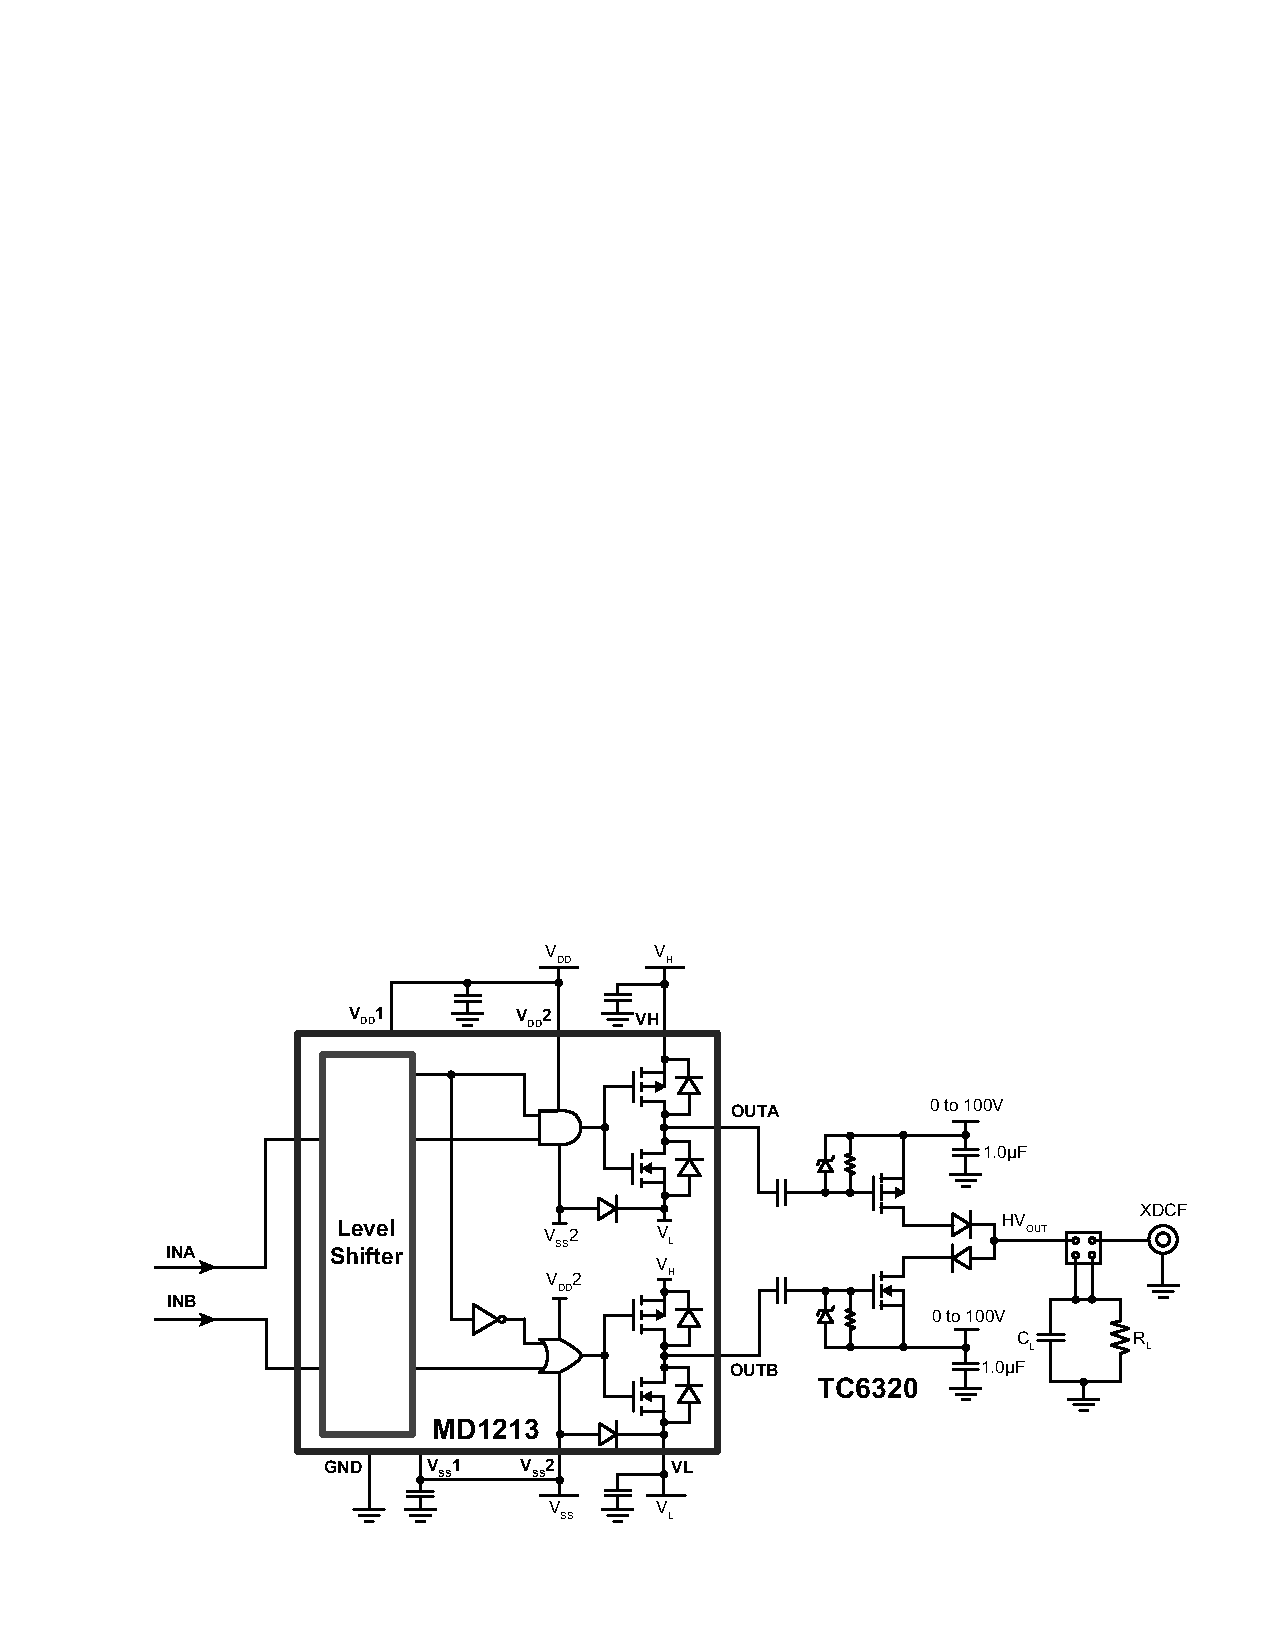
\includegraphics[width=\textwidth]{Figures/3_power_stage_block.pdf}
	\label{fig:3_power_stage}
	\caption[Block diagram of power stage]{Block diagram of power stage \cite{MD1213DB1}}
\end{figure}
Several MOSFET drivers were considered, e.g. ISL55111\cite{ISL55111}, EL7104\cite{EL7104}, and MD1213\cite{MD1213}. The MD1213 has an advantage over the ISL55111 or EL7104 for ultrasound MOSFET drivers since it is specifically designed for high-voltage P-channel and N-channel MOSFETs in medical ultrasound and other applications needing a high output current for a capacitive load. It has a high-speed input stage with a logic interface that can function from \qtyrange{1.8}{5}{\volt} and an ideal operating input signal range of \qtyrange{1.8}{3.3}{\volt}. The DC-coupled adaptive threshold circuit sets the level translator switch threshold to the average of the input logic \gls{low} and logic \gls{high} levels. Consequentially, the MD1213 is designed primarily for driving MOSFETs in medical ultrasound applications, whereas the ISL55111 and EL7104 are more general-purpose drivers that may not perform as well in ultrasound applications. The MD1213's output stage has a distinguishing feature in that the \gls{low} and \gls{high} levels of the output signal may be set independently of the rest of the circuit's supply voltages. The input logic levels, for example, might be \qty{0}{\volt} and \qty{1.8}{\volt}, whereas the control logic is powered by \qtyrange[retain-explicit-plus]{+5}{-5}{\volt}. The output \gls{low} and \gls{high} values, on the other hand, may be changed between \qtyrange[retain-explicit-plus]{-5}{+5}{\volt}. This gives you greater flexibility in adjusting the output signal levels to meet individual needs. The output stage may also provide peak currents of up to \qty{2}{\ampere}, depending on the load capacitance and supply voltages employed. Seen in \cref{fig:3_power_stage} is the circuit diagram of the power stage with the gate driver on the left side and the half-bridge on the right side.
\begin{figure}[htbp]
	\centering
	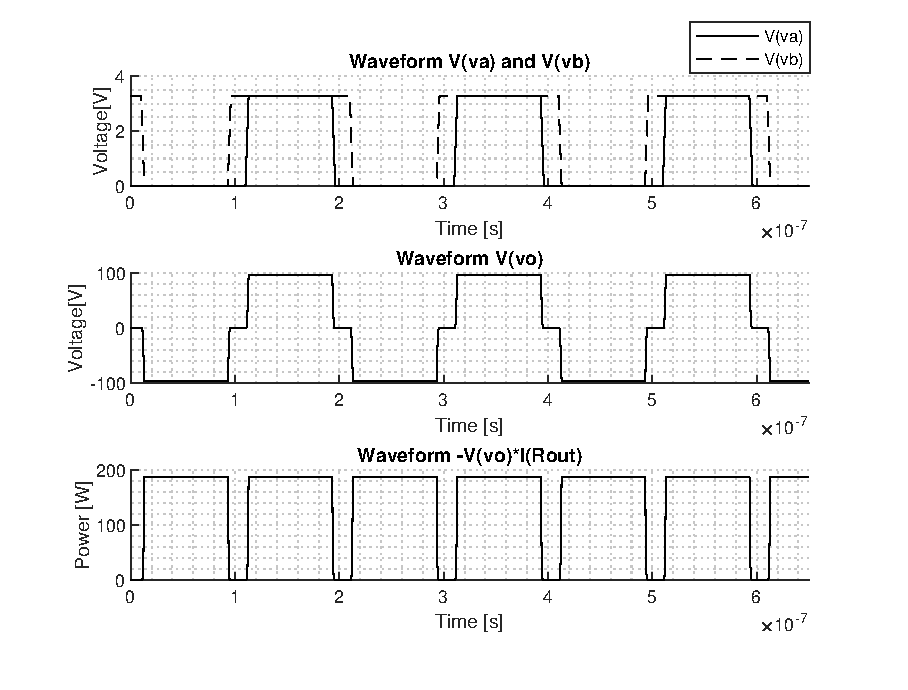
\includegraphics[width=.8\textwidth]{Figures/3_transmitter_sim_out.eps}
	\caption[LTspice simulation output of transmitter]{LTspice simulation output of transmitter with level shifter and half-bridge power stage from \cref{fig:app_ltspice_transmitter}}
	\label{fig:3_transmitter_sim}
\end{figure}
Using a \gls{spice} macro model, an LTspice simulation of the power stage was implemented where the full model can be seen in \cref{fig:app_ltspice_transmitter}. The resulting waveforms are seen in \cref{fig:3_transmitter_sim}. In the top subplot, the input voltages \texttt{INA} and \texttt{INB} are seen with their dead-time visible on each overlapped on period. Since \texttt{INB} is driving an N-channel \gls{mosfet}, the driving pulse train should be thought of as having the opposite polarity. When looking at the middle subplot, it is noted that dead time is visible as the time when the output voltage is zero. Thus, during that time neither \gls{fet} are allowing a current to pass, and therefore the voltage across the load is equal to zero. The lower subplot shows the maximum ideal power delivery using the peak pulse voltage, assuming the load is equal to \qty{50}{\ohm}. In reality, due to the laboratory instruments available for experiments, the pulse peak voltage will be less than $\pm \qty{100}{\volt}$.

\section{Transmit/Receive Switch}
\begin{figure}[htbp]
	\centering
%	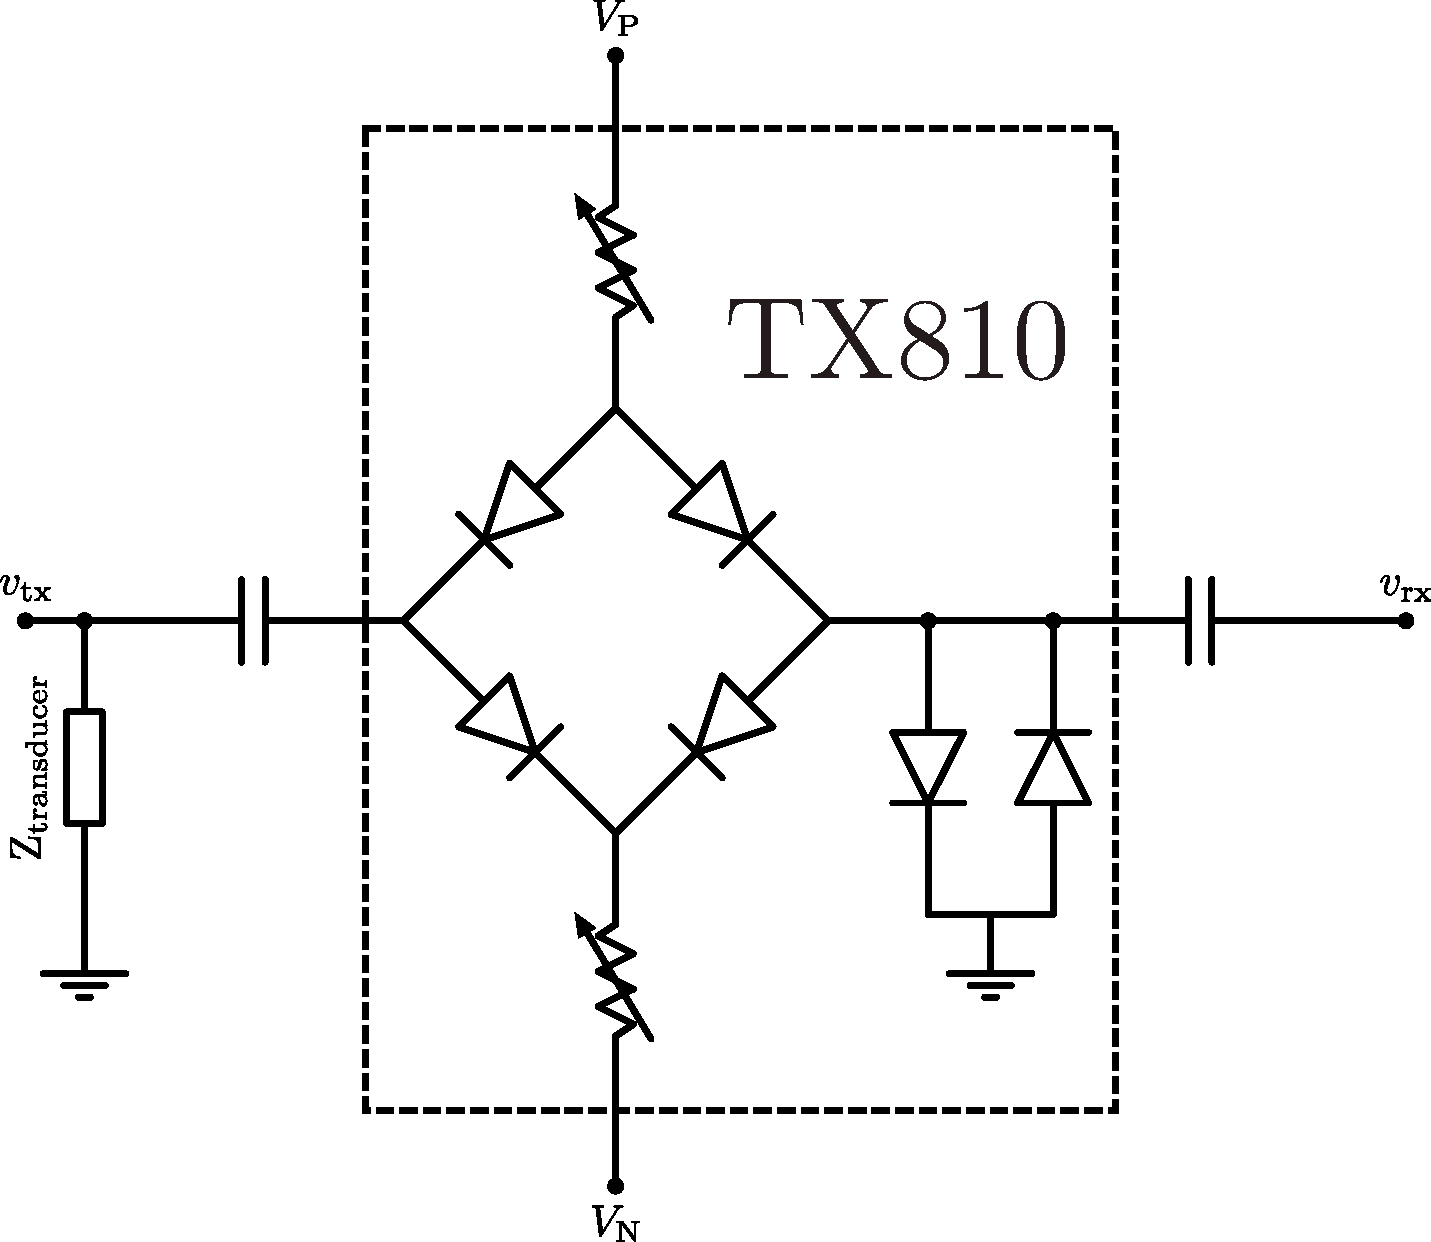
\includegraphics[width=.8\textwidth]{circuits/switch.pdf}
	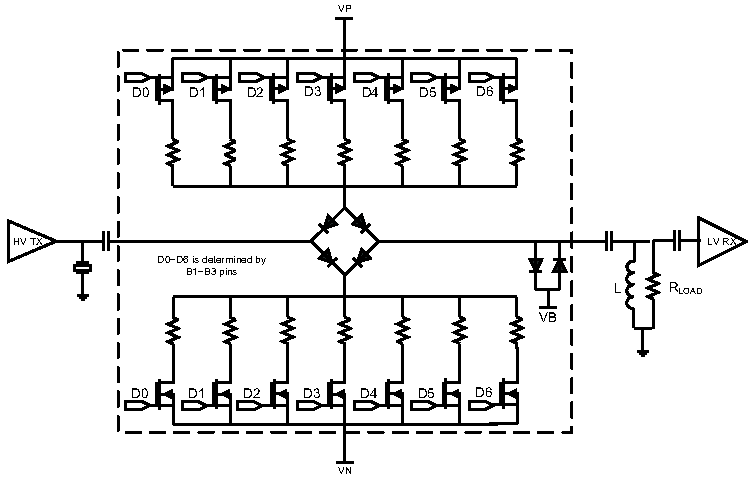
\includegraphics[width=.8\textwidth]{Figures/3_switch_tx810_block.pdf}
	\caption[Block diagram of TX/RX switching circuit]{Block diagram of TX/RX switching circuit where the inputs D1 through D6 are binary decoded from inputs $B_1$, $B_2$, $B_3$ \cite{TX810}}
	\label{fig:3_switch}
\end{figure}
Among the design considerations for the transmit and receive switch were the TX810\cite{TX810} and MD0101\cite{MD0101}. Both ICs are acceptable choices, however, the MD0101 is a newer and generally better choice since it has a lower insertion loss, which means that less of the ultrasound signal is lost as it passes through the switch. This results in a higher-quality image with a better signal-to-noise ratio. Additionally, MD0101 has a wider bandwidth, which means that it can transmit and receive ultrasound signals over a broader range of frequencies. However, since the TX810 is in stock and is also acceptable, it was chosen for the design. TX810 is an IC from Texas Instruments that can be used to switch transmit and receive paths of an ultrasound system. The IC fundamentally works by having a 3-bit programmable pin interface that will open and close the switch with a variable bias current. See \cref{fig:3_tx810_timing} for a visualisation of the switching operation, where \texttt{INPUT} is the incoming Doppler waveform being picked up from the transducer, \texttt{B3/B2/B1} is the switching signal closing the switch and thereby going in receive mode, and \texttt{OUTPUT} is the received signal seen in the \gls{afe}. When high-voltage transmitter signals are applied to the input, the internal diodes limit the output voltage. While in receive mode, the TX810's insertion loss is minimized. The TX810 features a 3-bit interface that may be used to program bias current from \qty{7}{\milli\ampere} to \qty{0}{\milli\ampere} for varying performance and power requirements, unlike conventional T/R switches. The device is put up in power-down mode when the TX810 bias current is set to \qty{0}{\milli\ampere} (high-impedance mode). The TX810 does not put a significant load on high-voltage transmitters when operating in the high-impedance mode.
\begin{figure}[htbp]
	\centering
	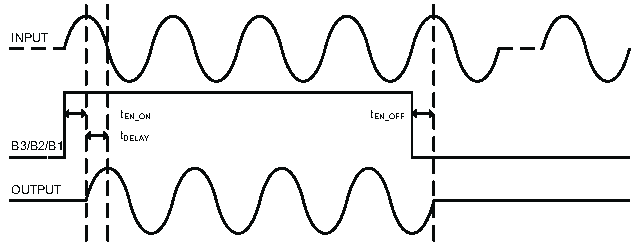
\includegraphics[width=.8\textwidth]{Figures/3_tx810_timing.pdf}
	\caption[Timing diagram of switching interface]{Timing diagram of switching interface where $t_{\mathrm{EN\_ON}}=\qty{0.6}{\micro\second}$, $t_{\mathrm{EN\_OFF}}=\qty{2.4}{\micro\second}$, and $t_{\mathrm{DELAY}}=\qty{1.3}{\nano\second}$ for the condition $B_1=B_2=B_3$ \cite{TX810}}
	\label{fig:3_tx810_timing}
\end{figure}

\begin{figure}[htbp]
	\centering
	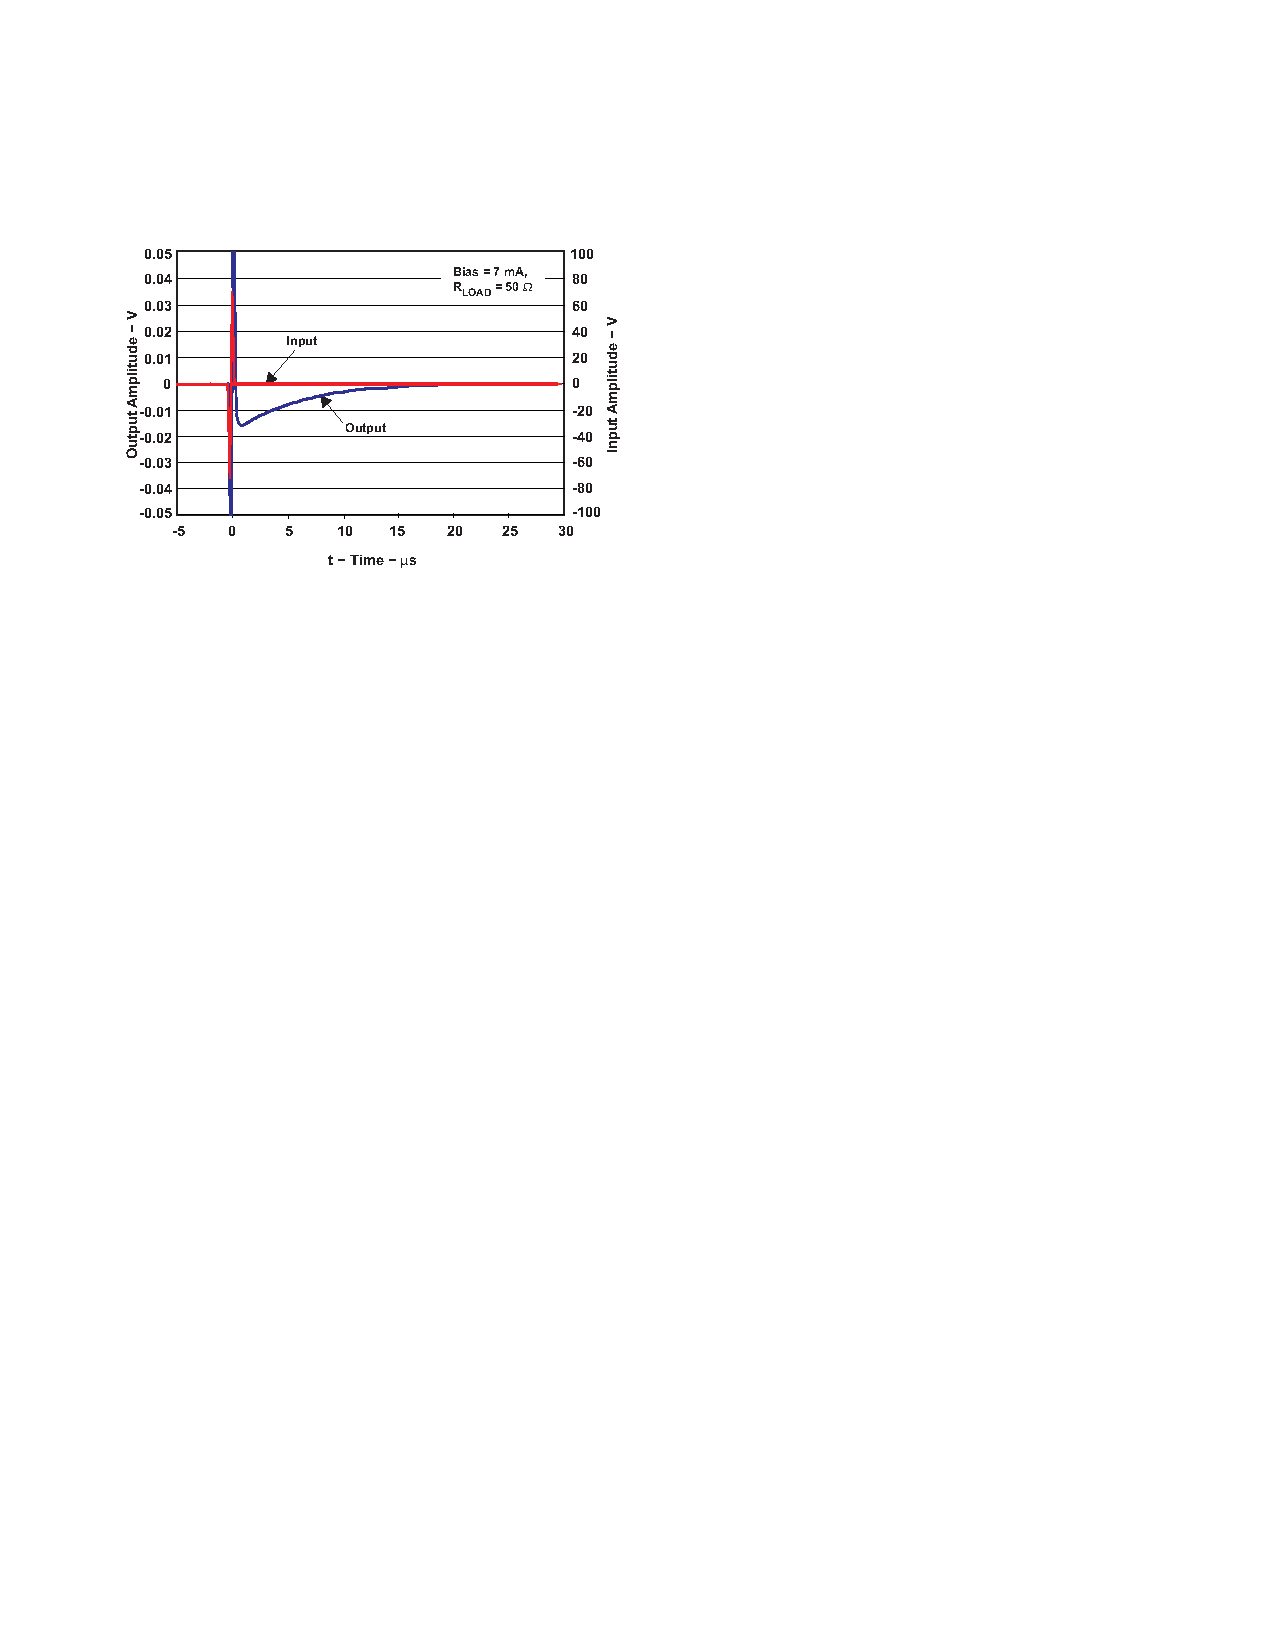
\includegraphics[width=.8\textwidth]{Figures/3_tx810_recovery.pdf}
	\caption[Recovery time from transmitting to receiving state with an AC coupled high-voltage pulse and TX810]{Recovery time from transmitting to receiving state with an AC coupled high-voltage pulse and TX810 \cite{TX810}}
	\label{fig:3_switch_recovery}
\end{figure}
Seen in \cref{fig:3_switch_recovery} is the recovery time between transient states in the TX810 diode bridge where the red curve is the input and blue is the output signal. According to the specified output curve, it takes approximately \qty{15}{\micro\second} to recover from the transmitting pulse. Thus, back-calculating to find the minimum distance to reliably receive an undisturbed signal is proportional to \cref{eq:tx810_recovery}.
\begin{subequations} \label{eq:tx810_recovery}
\begin{align}
	d &= \frac{c \cdot t}{2} \Longrightarrow \\
	d &= \frac{\qty{1480}{\meter\per\second} \cdot \qty{15}{\micro\second}}{2} = \qty{11.55}{\milli\meter}
\end{align}
\end{subequations}
Where $d$ is equal to the travel distance from the transducer to the scatterer, $c$ is the speed of sound in water (assumed to be \qty{1480}{\meter\per\second}), and $t$ is the recovery time as specified in  \cref{fig:3_switch_recovery}. The reason for dividing the distance by half is because the travel time is double the distance since the acoustic wave has to travel the distance from the transducer and the reflected wave has to travel back the equal distance. This means that a distance of less than \qty{11.55}{\milli\meter} to a scatterer is likely to produce an unreliable measurement. The ultrasound switch is designed to switch the transmit and receive paths at specific times, as determined by the input signals. A PCB design was implemented in Altium Designer \cite{altium} utilising three channels of the maximum eight available channels in the IC. Seen in \cref{fig:3_ultrasoundswitch} is a 3D render of the designed PCB.

\begin{figure}[htbp]
	\centering
	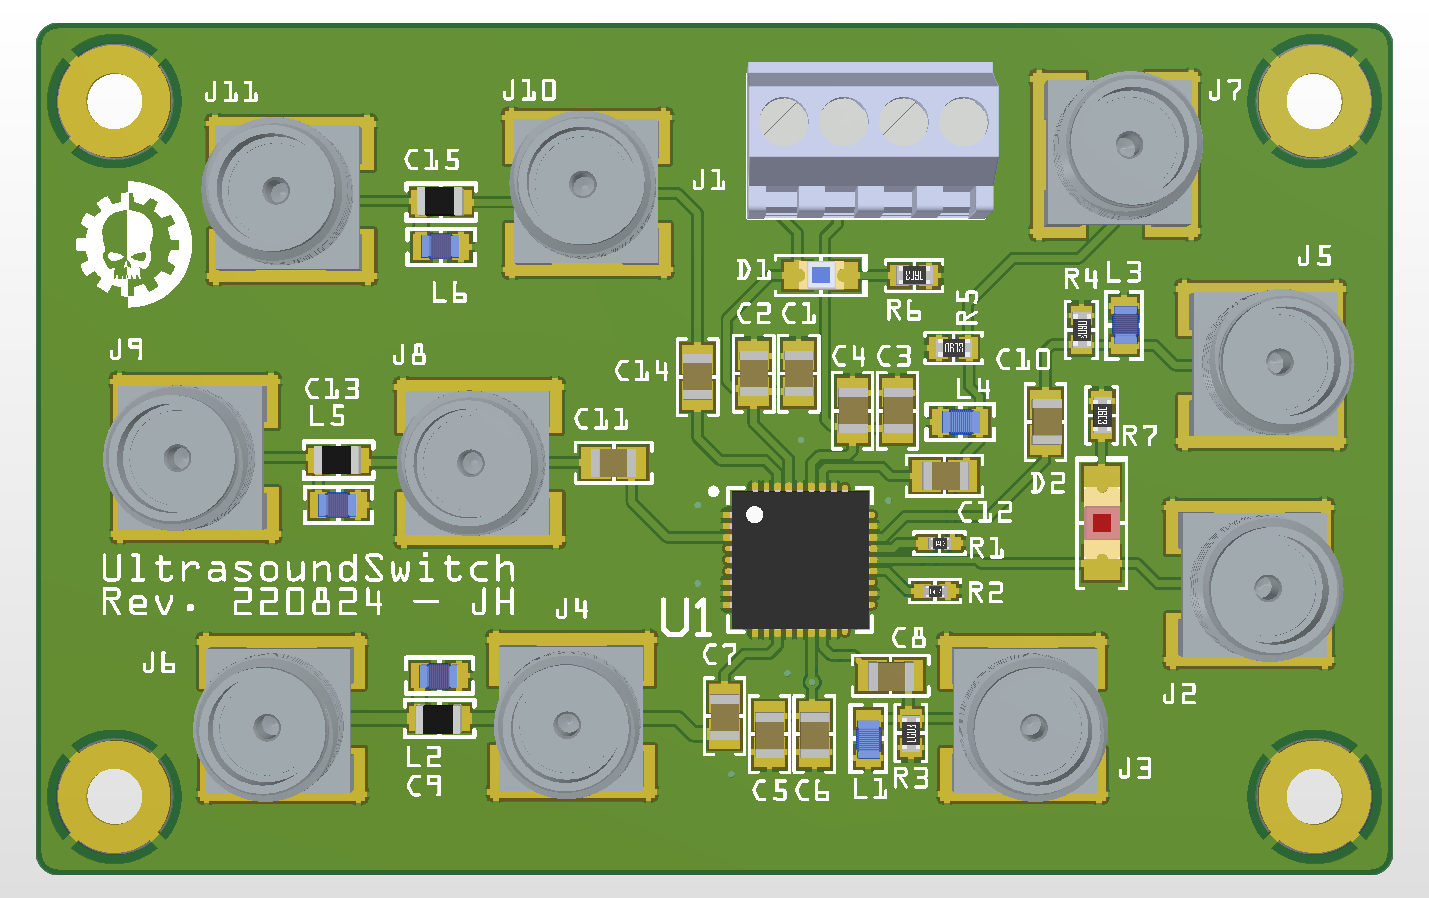
\includegraphics[width=.8\textwidth]{Figures/3_ultrasoundswitch.png}
	\caption{3D Render of PCB in Altium Designer}
	\label{fig:3_ultrasoundswitch}
\end{figure}
The module is designed with three usable channels, either three separate transducers for multi-angle sonography, or a \gls{cmut} with three channels in a single angle. However, in the following experiments with the TX/RX switch, only one channel will be used for simplifying the data acquisition experiments.

\section{Band-pass Filter}
\begin{figure}[htbp]
	\centering
	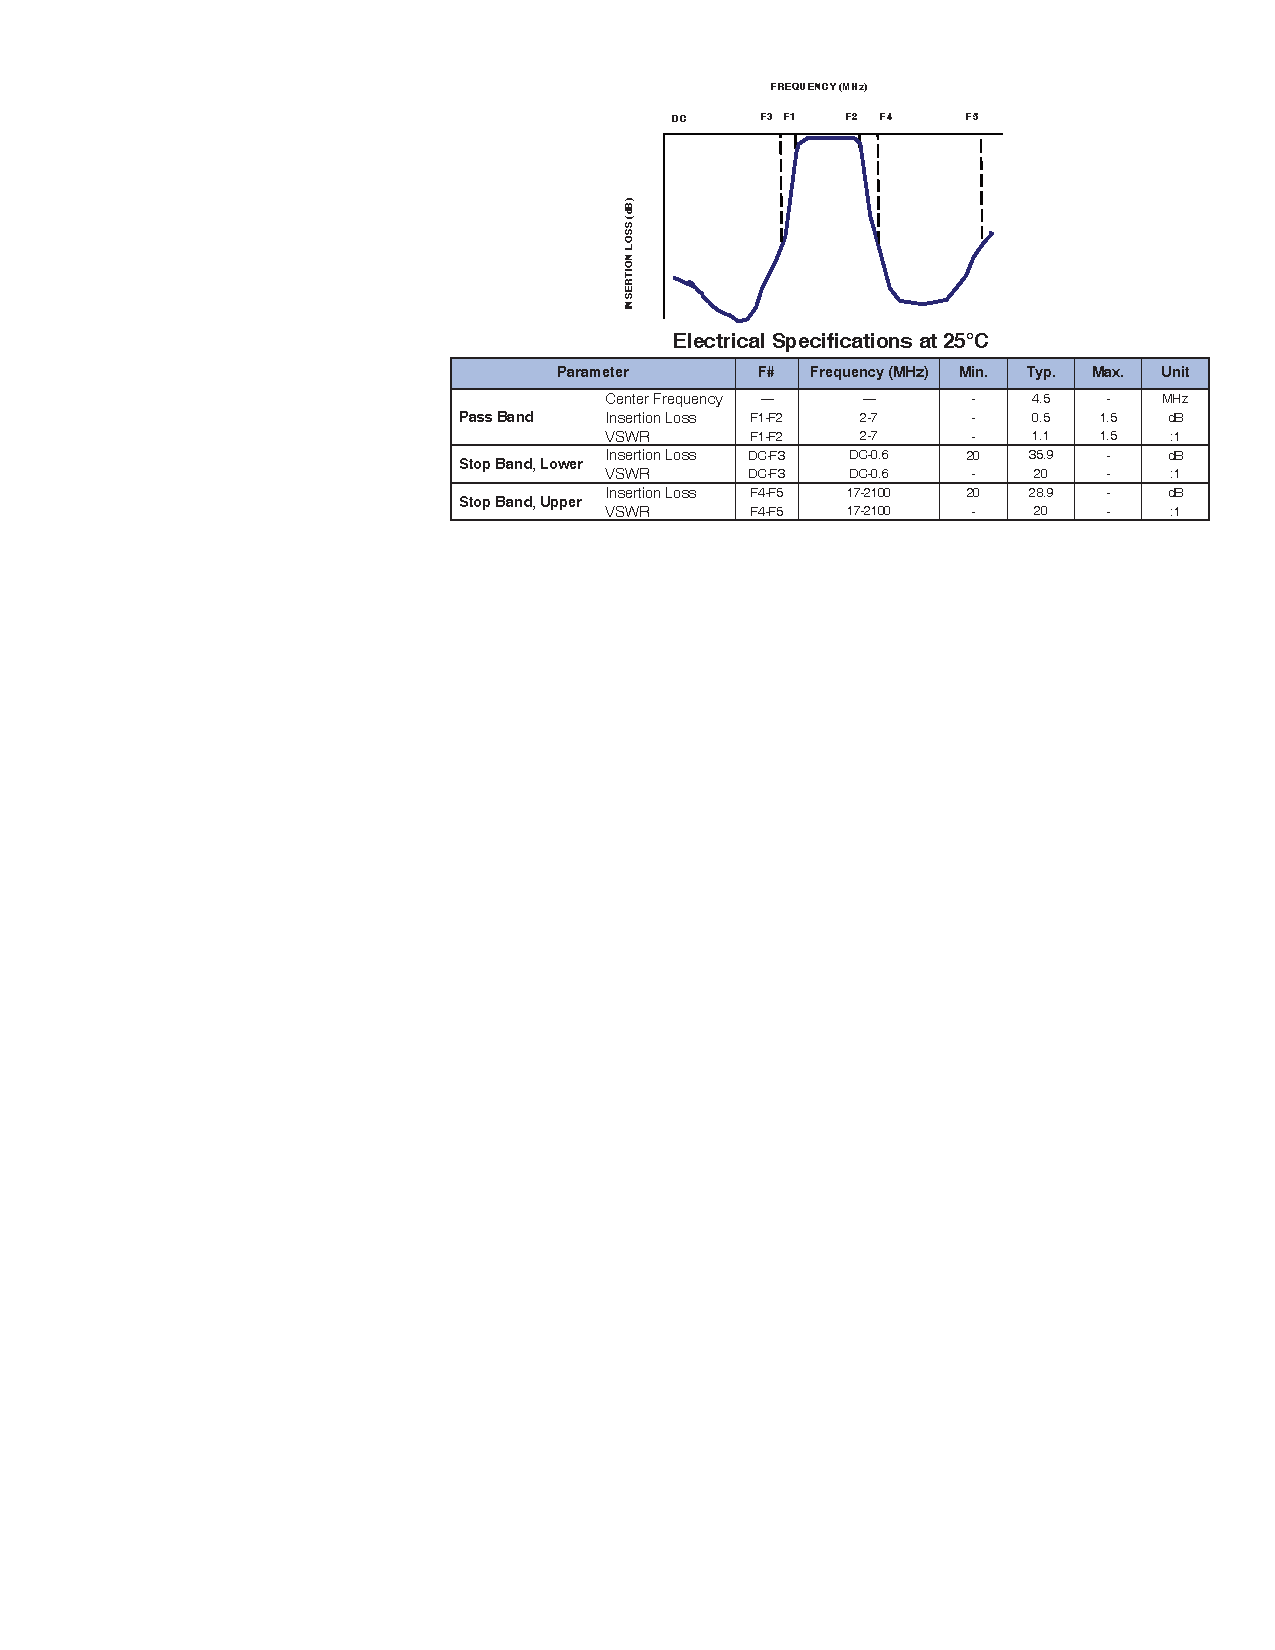
\includegraphics[width=\textwidth]{Figures/3_bpf_specs.pdf}
	\caption[Band-Pass Filter insertion loss and specifications]{Band-Pass Filter with (above) insertion loss showing a pass band of \qtyrange{2}{7}{\mega\hertz} of \qty{0.5}{\decibel} insertion loss and (below) electrical specifications showing the minimum stopband attenuation of \qty{20}{\decibel} \cite{BPF}}
	\label{fig:3_bpf_specs}
\end{figure}
After the signal is received, it is filtered with a \gls{bp} filter to remove unwanted noise and interference from the received signal. The presence of these unwanted frequency components can distort the received signal and reduce the quality of the resulting imaging. The specs from the datasheet of used modular component BPF-C4R5+ \cite{BPF} are seen in \cref{fig:3_bpf_specs}. Filtering the received signal through this device means that any signals produced by the transducer at frequencies outside the range of interest will be attenuated. An ultrasound receiver requires a band-pass filter to enable only the frequencies within a predetermined range to pass through while blocking out frequencies outside that range. Using the specs and S21 forward transmission coefficient data, a bode plot can be visualised in \cref{fig:3_bpf_s21_bode_plot}.

\begin{figure}[htbp]
	\centering
	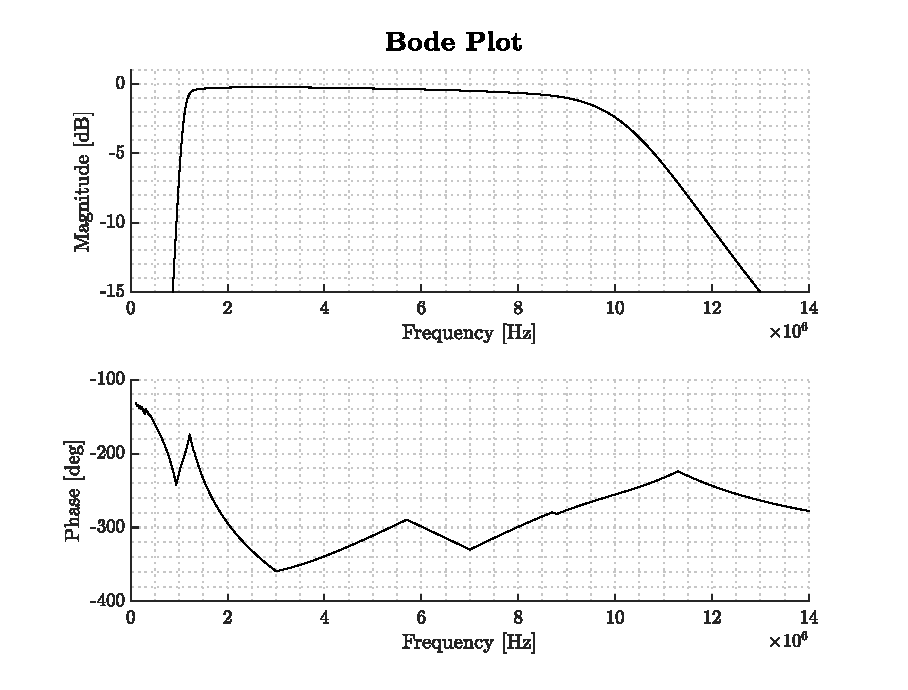
\includegraphics[width=.8\textwidth]{Figures/3_bpf_s21_vals.eps}
	\caption[Bode plot of bandpass filter]{Bode plot of BPF-C4R5+ S21 forward transmission coefficient of the active filter as specified by the manufacturer}
	\label{fig:3_bpf_s21_bode_plot}
\end{figure}

\section{Preamplifier}
\begin{figure}[htbp]
	\centering
	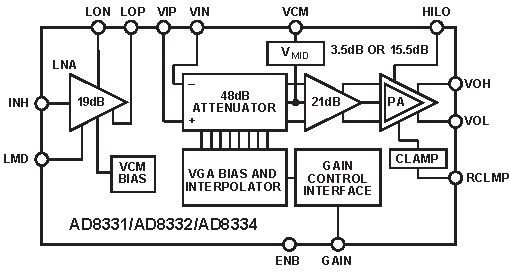
\includegraphics[width=.8\textwidth]{Figures/3_ad8332_block.pdf}
	\caption[Block diagram of preamplifier AD8332]{Block diagram of preamplifier AD8332 \cite{AD8332}}
	\label{fig:3_preamplifier_block}
\end{figure}
The isolated signal is still rather weak to be measured using digital circuits, and therefore the amplitude must be increased with the preamplifier circuit. This circuit is based on the integrated circuit from Analog Devices AD8332 \cite{AD8332}, which is a device that combines a dual-channel \gls{lna} and \gls{vga}, designed specifically for ultrasound systems. A diagram of its internal functional blocks can be seen in \cref{fig:3_preamplifier_block}. The AD8332 functions at frequencies up to \qty{120}{\mega\hertz}. Each channel includes an ultralow noise preamp (\gls{lna}), a \gls{vga} with \qty{48}{\decibel} of gain range, and a selectable gain post amp with adjustable output limiting. The LNA gain is \qty{19}{\decibel} with a single-ended input and differential outputs. To match the signal source without sacrificing noise performance, the LNA input impedance can be adjusted using a single resistor. The VGA has low output-referred noise, which is useful in driving high-speed differential ADCs. The gain of the post amp can be pin-selected to \qty{3.5}{\decibel} or \qty{15.5}{\decibel}, depending on the converter requirements. The output can be limited to a user-defined clamping level to avoid input overload to a subsequent \gls{adc}, with the clamping level adjusted using an external resistor. A SPICE macro model is provided by the vendor and the preamplification is successfully simulated using LTspice with the full LTspice model found in \cref{fig:app_ltspice_preamp}, and the probed inputs and outputs seen in \cref{fig:3_preamplifier_sim}.

\begin{figure}[htbp]
	\centering
	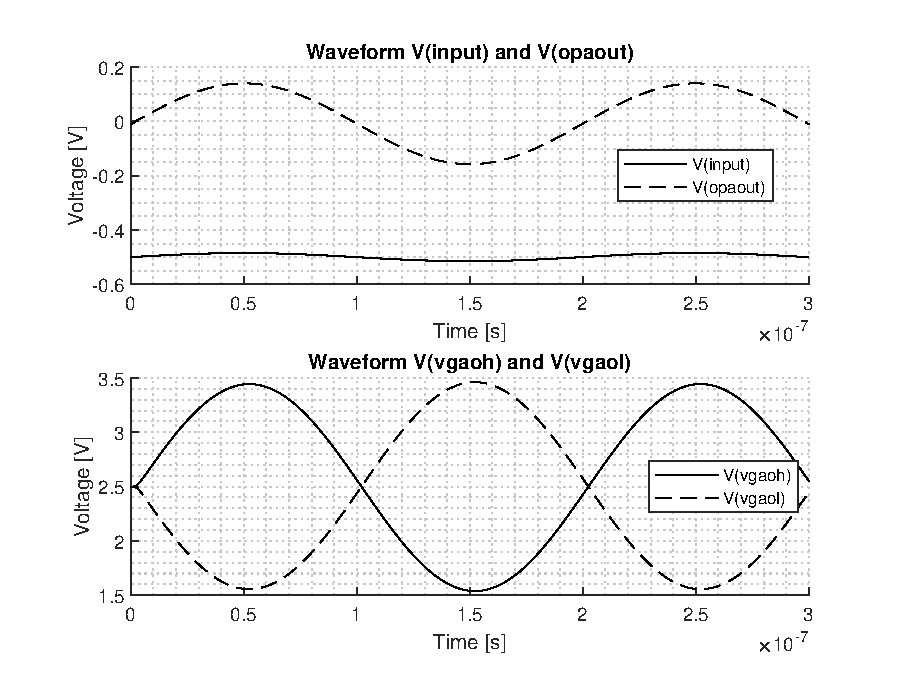
\includegraphics[width=.8\textwidth]{Figures/3_preamplifier_sim_out.eps}
	\caption[LTspice simulation output of preamplifier]{LTspice simulation output of preamplifier \gls{lna} and \gls{vga} from \cref{fig:app_ltspice_preamp}}
	\label{fig:3_preamplifier_sim}
\end{figure}

\section{Quadrature Demodulator}
\begin{figure}[htbp]
	\centering
	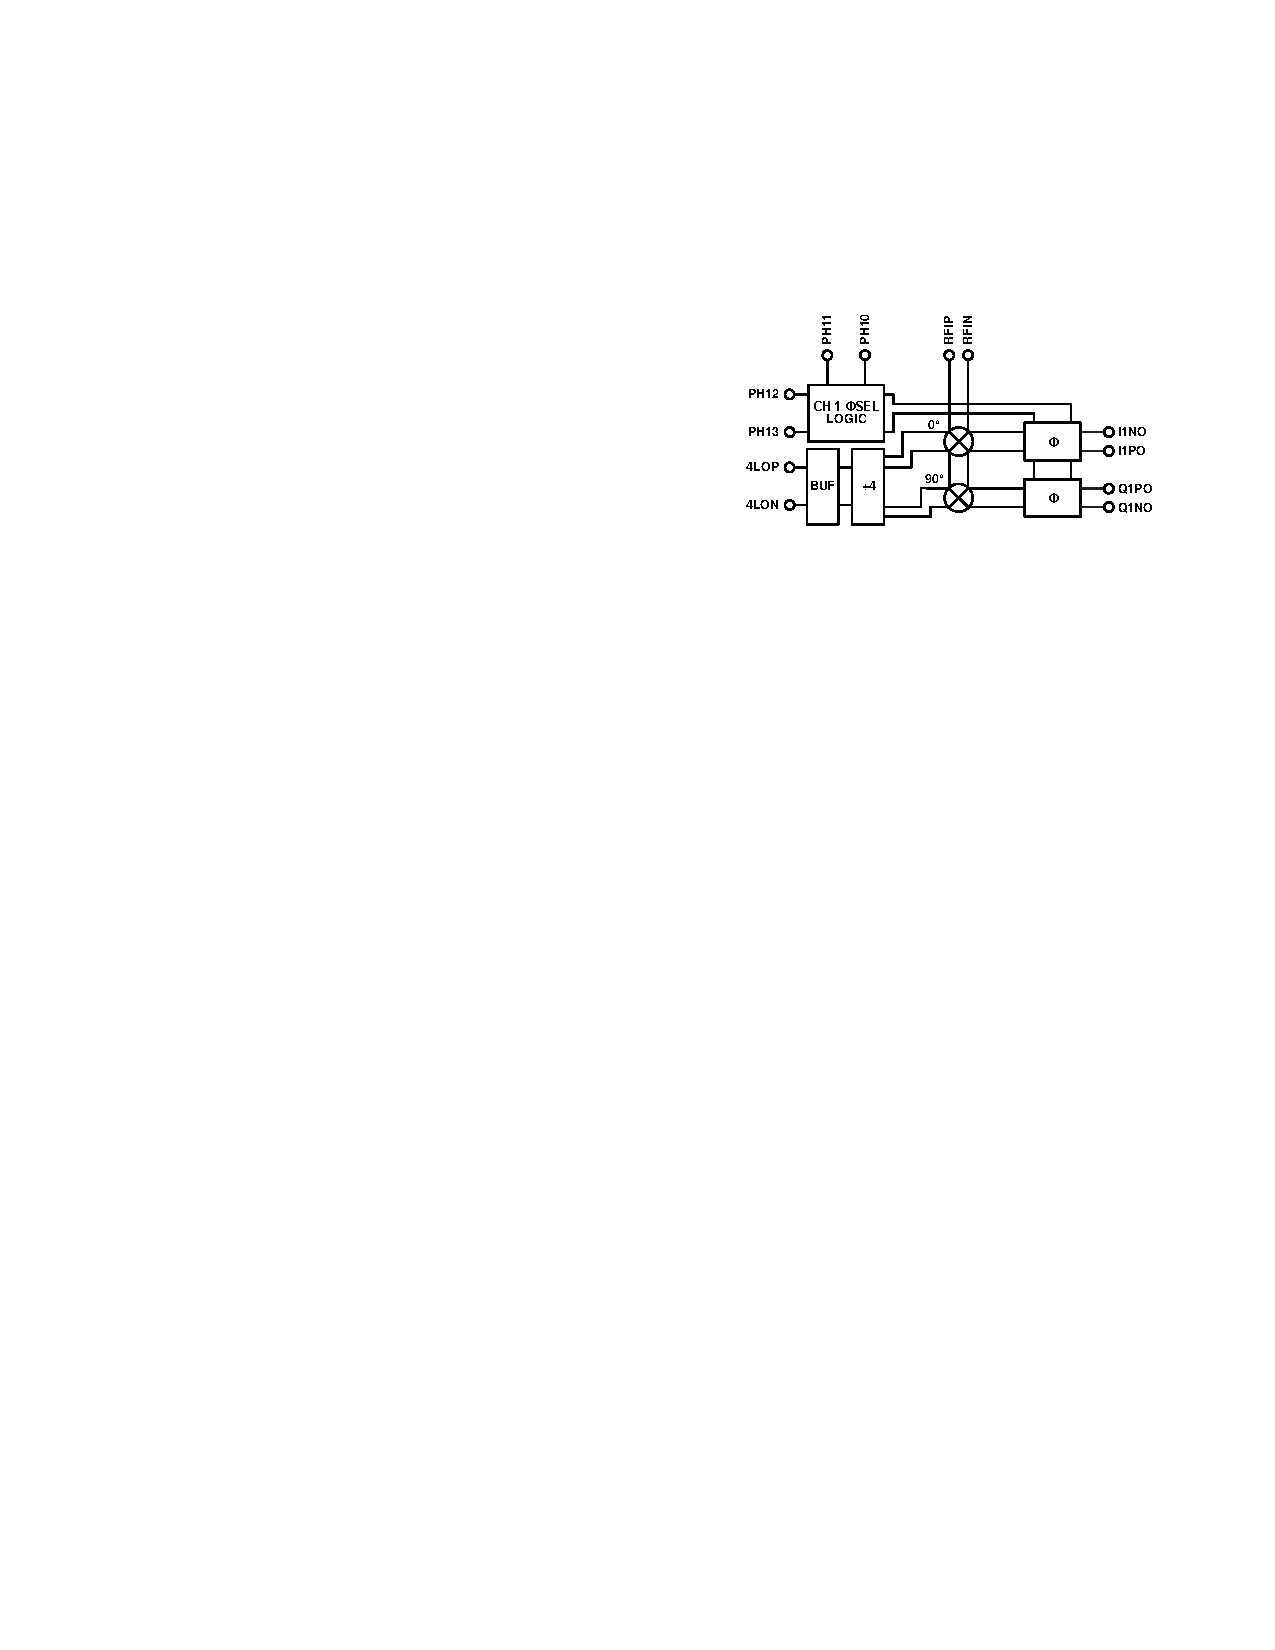
\includegraphics[width=.8\textwidth]{Figures/3_ad8333_block.pdf}
	\caption[Block diagram of demodulator AD8333]{Block diagram of demodulator AD8333 \cite{AD8333}}
	\label{fig:3_demodulator_block}
\end{figure}
After the preamplifier, the amplified signal must be demodulated to prepare it for sampling. The device used for quadrature demodulation is an integrated circuit from Analog Devices AD8333 \cite{AD8333} I/Q demodulator. A diagram of the internal functional blocks can be seen in \cref{fig:3_demodulator_block} where the primary inputs are \texttt{RFIP} and \texttt{RFIN}, which are the two differential RF signals from the preamplifier. The RF inputs connect directly to the outputs of the LNA of the preamplifier. The internal \qty{0}{\degree} and \qty{90}{\degree} phases of the local oscillator (LO) are generated by a divide-by-4 circuit that drives the mixers of a matched I/Q demodulator pair. The I and Q outputs are presented as currents, making summation possible. The summed current outputs are then converted to voltages by a high dynamic range, current-to-voltage (I-V) converter, such as the AD8021 \cite{AD8021}, which functions as a trans-impedance amplifier. A SPICE macro model is provided by the vendor and the I/Q demodulation is successfully simulated using LTspice using the LTspice model found in appendix \cref{fig:app_ltspice_demod}, with the probed inputs and outputs seen in \cref{fig:3_demod_sim_in,fig:3_demod_sim_out}.

\begin{figure}[htbp]
	\centering
	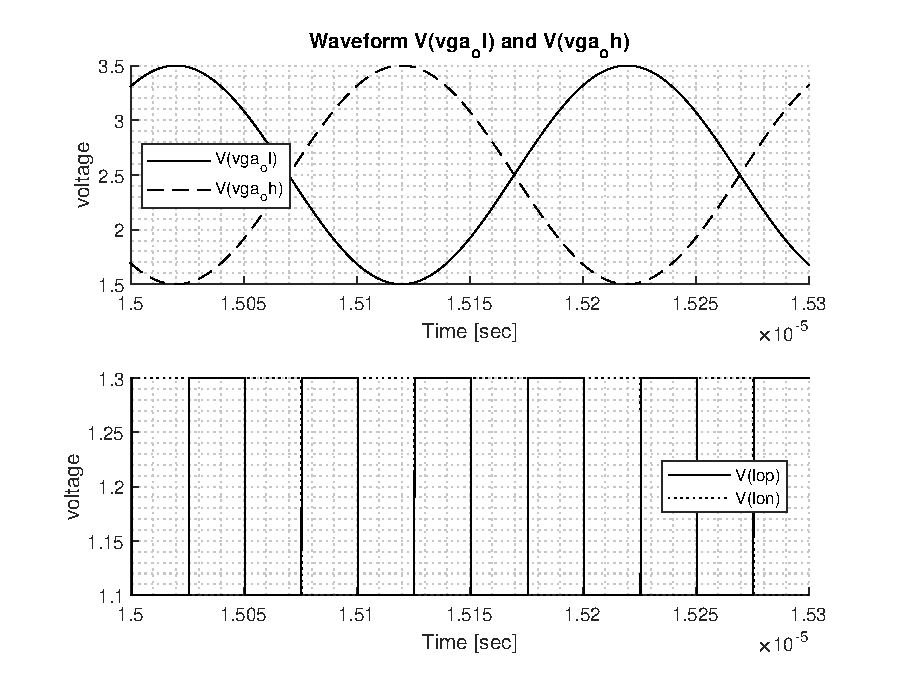
\includegraphics[width=.8\textwidth]{Figures/3_demod_sim_in.eps}
	\caption[LTspice simulation demodulator input variables]{LTspice simulation demodulator input variables from \cref{fig:app_ltspice_demod}}
	\label{fig:3_demod_sim_in}
\end{figure}
\begin{figure}[htbp]
	\centering
	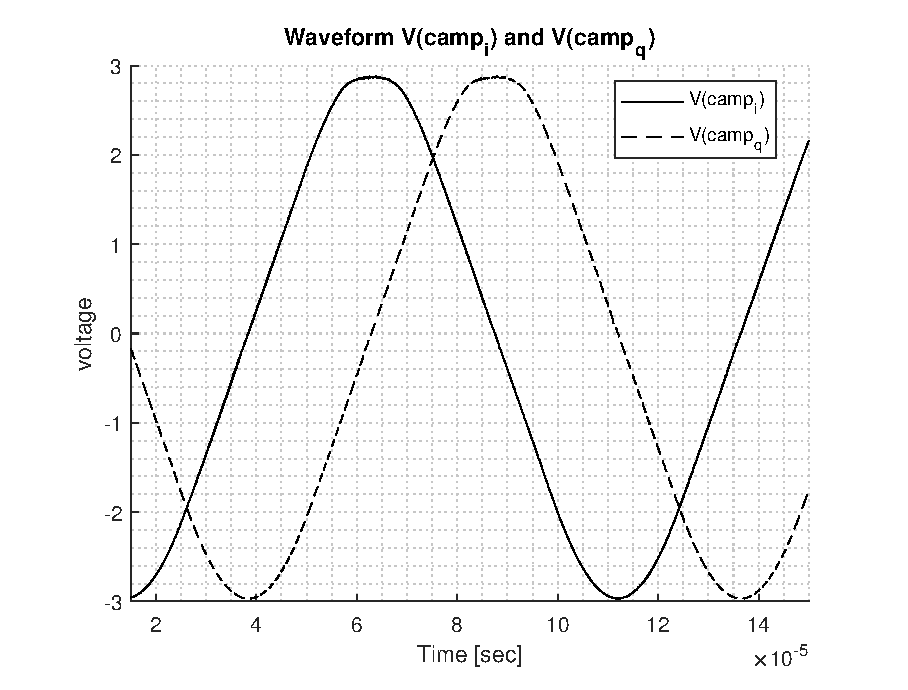
\includegraphics[width=.8\textwidth]{Figures/3_demod_sim_out.eps}
	\caption[LTspice simulation demodulator output variables]{LTspice simulation demodulator output variables Q and I voltages from \cref{fig:app_ltspice_demod}}
	\label{fig:3_demod_sim_out}
\end{figure}
\section{Sample and Hold}
\begin{figure}[htbp]
	\centering
	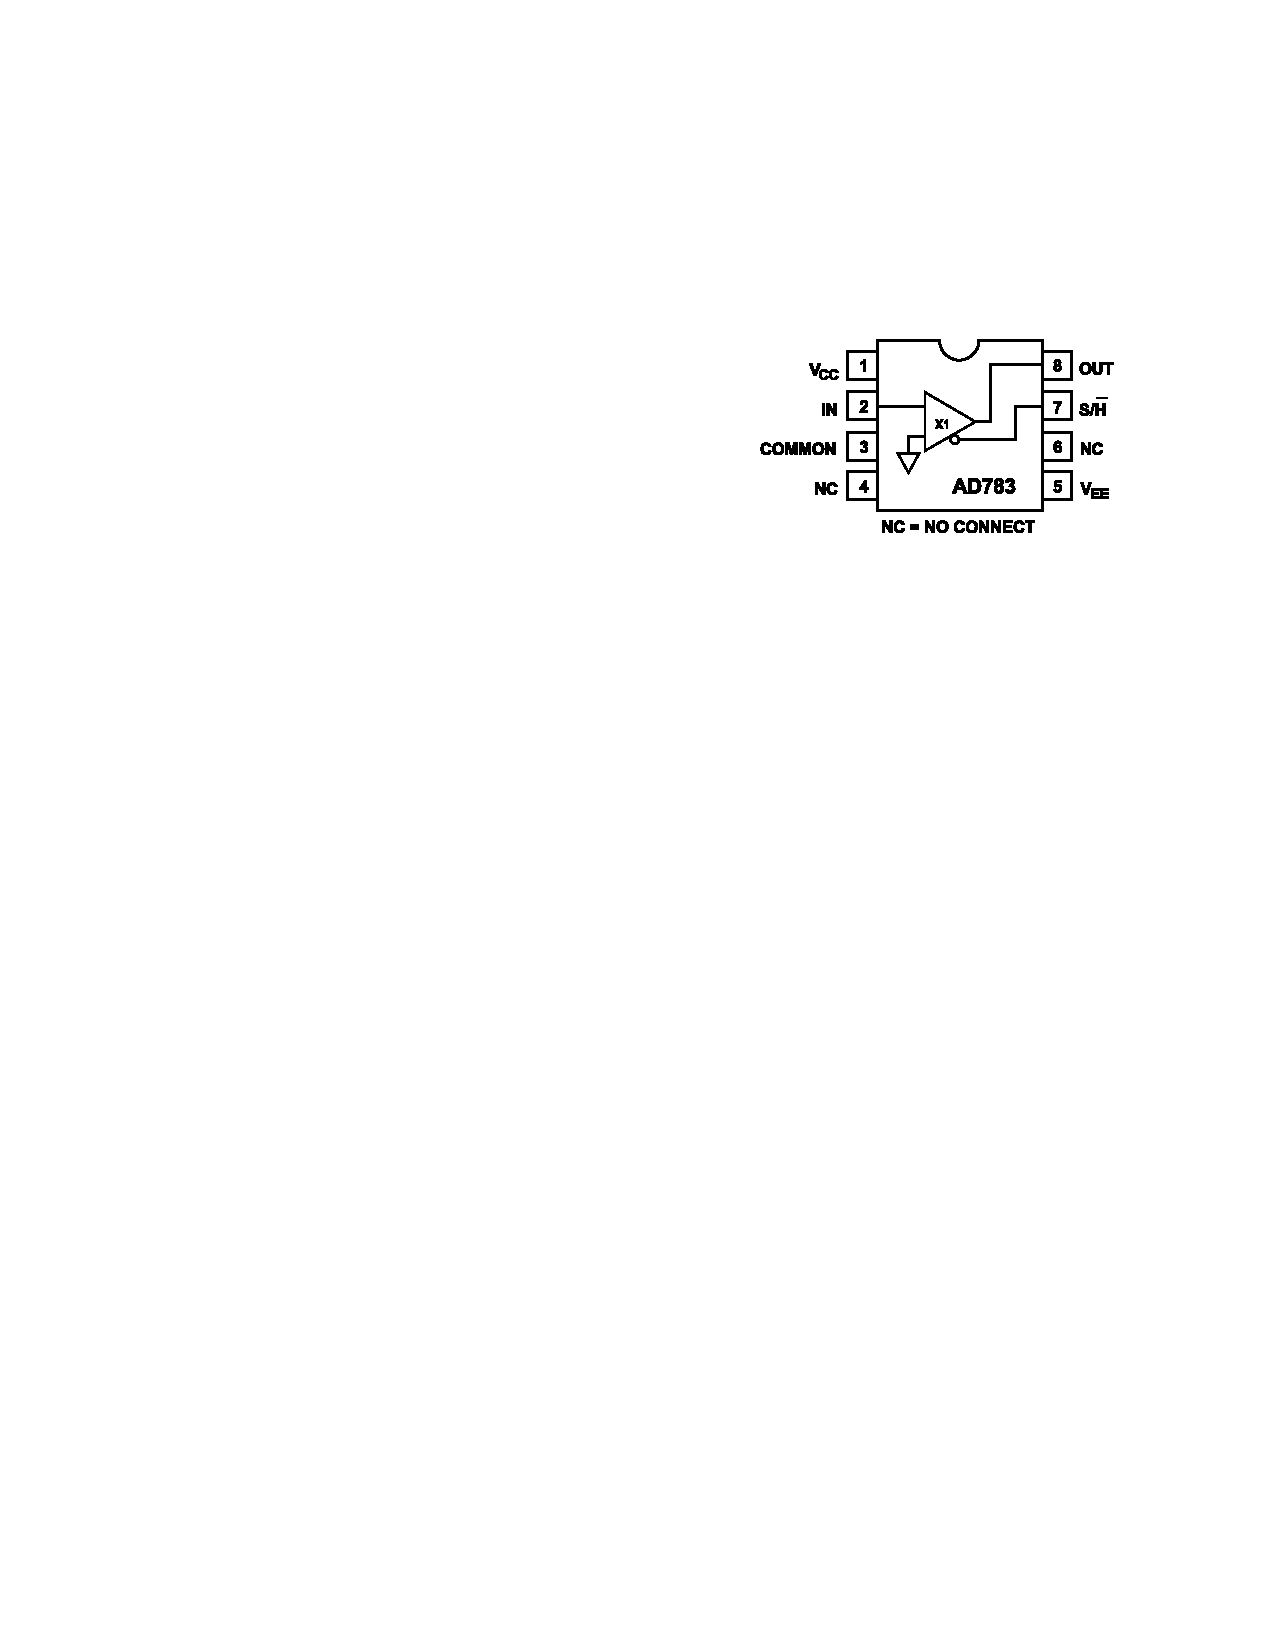
\includegraphics[width=.8\textwidth]{Figures/3_sample_hold_ad783.pdf}
	\caption[AD783 Sample and Hold amplifier block diagram]{AD783 Sample and Hold Amplifier functional block diagram \cite{AD783}}
	\label{fig:3_sha_block}
\end{figure}
In this system, the sample-and-hold amplifier is necessary to keep values between each sample line. In chapter 2, it was described how the pulsed-wave flow-meter measures the movement of scatterers by sampling the back-scattered signal at a specific depth. Generally, the intended use for this part is in general data acquisition systems such as an \gls{adc}. In that application, the sample-and-hold amplifier captures an analogue signal and retains it during certain operations, usually analogue-to-digital conversion. Through a S/H input, two possible modes are selected, \textit{sample} or \textit{hold}. During the sample mode of operation, the output of the sample-and-hold amplifier follows the input. During the hold mode of operation, the output may not change by more than 1 \gls{lsb}. The typical usage of a SHA is to keep the ADC input constant throughout the conversion process. With some types of ADCs, but not all, the input cannot change by more than 1 \gls{lsb} during the conversion, or else the process will be compromised. This can either impose very low-frequency limits on such ADCs or necessitate their use with a SHA to hold the input during each conversion. An internal capacitor forms the key component of the sample-and-hold amplifier, which serves as the energy storage device. The input amplifier buffers the input signal by presenting a high impedance to the signal source while providing current gain to charge the hold capacitor. In the sample mode, the voltage on the hold capacitor follows the input signal, albeit with some delay and bandwidth limitations. In the hold mode, the switch is opened, and the capacitor retains the voltage present before being disconnected from the input buffer. The output buffer prevents the held voltage from discharging too soon by offering a high impedance to the hold capacitor. The switching circuit and its driver work together to enable the SHA to alternate between sample and hold modes.

In the pulsed-wave flowmeter, the sample-and-hold amplifier is used to keep each sample value between each gate pulse. This is done for both the I and Q signals in parallel. A diagram of a sample-and-hold operation can be seen in \cref{fig:3_sha_function}.

\begin{figure}[htbp]
	\centering
	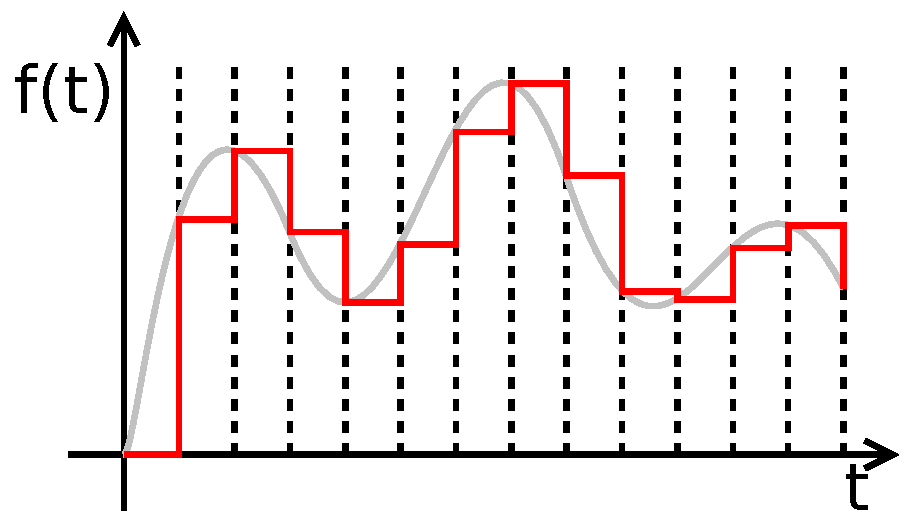
\includegraphics[width=.8\textwidth]{Figures/3_sample_hold_amplifier_quantization.pdf}
	\caption[Sample and Hold function with input function $f(t)$ over time]{Sample and Hold function with input function $f(t)$ over time \cite{sha_pic}}
	\label{fig:3_sha_function}
\end{figure}

\section{Active Filter, DC-Coupling}
\begin{figure}[htbp]
	\centering
	\begin{subfigure}[b]{0.49\textwidth}
		\resizebox{\textwidth}{!}{%
			\begin{circuitikz}
				\tikzstyle{every node}=[font=\normalsize]
				\draw (13,17.25) to[C,l={ \normalsize $C_2$}] (13,15.75);
				\draw (14.5,17.25) to[C,l={ \normalsize $C_3$}] (14.5,15.75);
				\draw (11.75,17.25) to[R,l={ \normalsize $R_2$}] (11.75,15.75);
				\draw [](11.75,17.25) to[short] (14.25,17.25);
				\draw [](14.25,17.25) to[short] (15.25,17.25);
				\draw [](15.25,16.25) to[short] (15.25,15.5);
				\draw [](15.25,15.5) to[short] (17.75,15.5);
				\draw [](17.75,15.5) to[short] (17.75,16.75);
				\draw (16.75,16.75) node[op amp,scale=1, yscale=-1 ] (opamp2) {};
				\draw (opamp2.+) to[short] (15.25,17.25);
				\draw  (opamp2.-) to[short] (15.25,16.25);
				\draw (17.95,16.75) to[short](18.25,16.75);
				\draw (17.75,16.75) to[short, -*] (17.75,16.75);
				\draw [](18.25,16.75) to[short, -o, l=$V_{\mathrm{bias}}$] (18.5,16.75);
				\draw (17.75,15.5) to[C,l={ \normalsize $C_4$}] (17.75,14.5);
				\draw (17.75,14.5) to (17.75,14.25) node[ground]{};
				\draw (10,17.25) to[american voltage source,l={ \normalsize $V_1$}] (10,15.75);
				\draw (10,15.75) to (10,15.5) node[ground]{};
				\draw [](11.75,15.75) to[short] (14.5,15.75);
				\draw (13,15.75) to (13,15.5) node[ground]{};
				\draw (13,15.75) to[short, -*] (13,15.75);
				\draw (10,17.25) to[R,l={ \normalsize $R_1$}] (11.75,17.25);
				\draw (17.75,15.5) to[short, -*] (17.75,15.5);
				\draw (11.75,17.25) to[short, -*] (11.75,17.25);
				\draw (13,17.25) to[short, -*] (13,17.25);
				\draw (14.5,17.25) to[short, -*] (14.5,17.25);
			\end{circuitikz}
		}%
		\caption{Circuit diagram of DC bias circuit}
		\label{fig:3_dc_bias_circuit}
	\end{subfigure}%
	\begin{subfigure}[b]{.49\textwidth}
		\resizebox{\textwidth}{!}{%
			\begin{circuitikz}
				\draw (9.75,15.75) to[sinusoidal voltage source, sources/symbol/rotate=auto,l={ \normalsize $V_{\mathrm{in}}$}] (9.75,17.75);
				\draw (9.75,15.75) to (9.75,15.5) node[ground]{};
				\draw (9.75,17.75) to[C,l={ \normalsize $C_1$}] (11.25,17.75);
				\draw (12.75,17.25) node[op amp,scale=1, yscale=-1 ] (opamp2) {};
				\draw (opamp2.+) to[short] (11.25,17.75);
				\draw  (opamp2.-) to[short] (11.25,16.75);
				\draw (13.95,17.25) to[short](14.25,17.25);
				\draw (11.25,17.75) to[short, -*] (11.25,17.75);
				\draw (14,17.25) to[R,l={ \normalsize $R_3$}] (14,16);
				\draw[] (14,16) to[short] (11.25,16);
				\draw [](11.25,16) to[short] (11.25,16.75);
				\draw [](14.25,17.25) to[short, -o, l=$V_{\mathrm{out}}$] (14.5,17.25);
				\draw [](14,16) to[short] (14,15.5);
				\draw (14,15.5) to[R,l={ \normalsize $R_4$}] (12.75,15.5);
				\draw (12.75,15.5) to[C,l={ \normalsize $C_5$}] (11.75,15.5);
				\draw (11.75,15.5) to (11.5,15.5) node[ground]{};
				\draw (14,17.25) to[short, -*] (14,17.25);
				\draw [](11.25,17.75) to (11.25,18) node[vcc]{\normalsize $V_{\mathrm{bias}}$};
			\end{circuitikz}
		}%
		\caption{Circuit diagram of \gls{hp}, \gls{prf} and Wall filter}
		\label{fig:3_prf_wall_diagram}
	\end{subfigure}
\end{figure}
Finally, the signal should be DC coupled for sampling and filtered using an active \gls{hp} filter to remove unwanted PRF frequency and wall frequency. For generating a DC bias voltage, the circuit in \cref{fig:3_dc_bias_circuit} is used. Here, a voltage divider is coupled with some stabilising capacitors and a voltage follower to output a stable output. In the circuit diagram in \cref{fig:3_prf_wall_diagram}, a \gls{hp} filter is used as a combined \gls{prf} and Wall-filter in conjunction with a \qty{2}{\decibel} gain amplification to maximize the dynamic range of the \gls{adc} measurements from \qtyrange{0}{3.3}{\volt}. In the diagram, $V_{bias}=\qty{1.65}{\volt}$, which is half of the \gls{adc} dynamic range of \qtyrange{0}{3.3}{\volt}, and $v_{\mathrm{in}}$ is the input signal to the filter from the output of the sample-and-hold amplifier. To get a \qty{1.65}{\volt} DC-bias, a voltage-follower op-amp configuration is used with a voltage divider input on the supply voltage of \qty{5}{\volt}, outlined in \cref{eq:3_dc_couple_voltage}.
\begin{equation} \label{eq:3_dc_couple_voltage}
	V_{\mathrm{dc}}= V_{\mathrm{cc}} \cdot \frac{R_{2}}{R_{1}+R_{2}} = \qty{5}{\volt} \cdot \frac{\qty{5}{\kilo\ohm}}{\qty{10}{\kilo\ohm}+\qty{5}{\kilo\ohm}} = \qty{1.66}{\volt}
\end{equation}
For the \qty{2}{\decibel} gain, a non-inverting amplifier configuration is used, expressed by \cref{eq:3_dc_couple_gain}.
\begin{equation} \label{eq:3_dc_couple_gain}
	G_{\unit{\decibel}} = \frac{V_{\mathrm{out}}}{V_{\mathrm{in}}} = 20\cdot \log_{10} \left(1 + \frac{R_3}{R_4} \right) = 20\cdot \log_{10} \left( 1 + \frac{\qty{40}{\kilo\ohm}}{\qty{150}{\kilo\ohm}} \right) = \qty{2.05}{\decibel}
\end{equation}
A SPICE simulation was implemented and can be seen in \cref{fig:app_ltspice_dc_coupler}. From this simulation model, a small signal analysis as well as a transient analysis was conducted. The resulting small signal analysis can be seen in \cref{fig:3_dccoupler_sim_ac} and the transient analysis can be seen in \cref{fig:3_dccoupler_sim_transient} and confirms the expected result.
\begin{figure}[htbp]
	\centering
	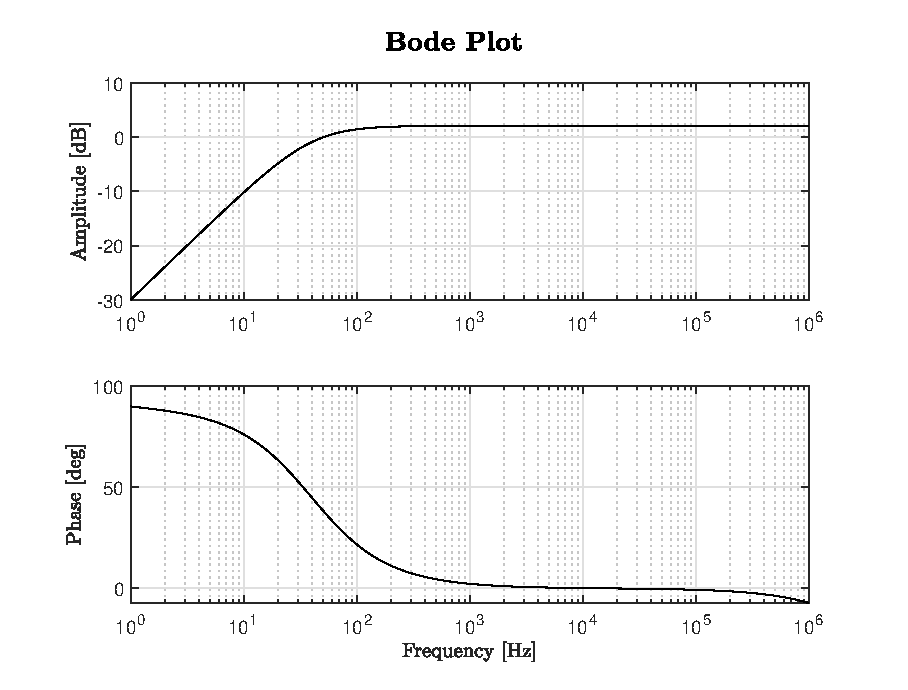
\includegraphics[width=.8\textwidth]{Figures/3_dc_coupler_sim.eps}
	\caption{Small-signal analysis of DC-Coupling filter circuit}
	\label{fig:3_dccoupler_sim_ac}
\end{figure}
\begin{figure}[htbp]
	\centering
	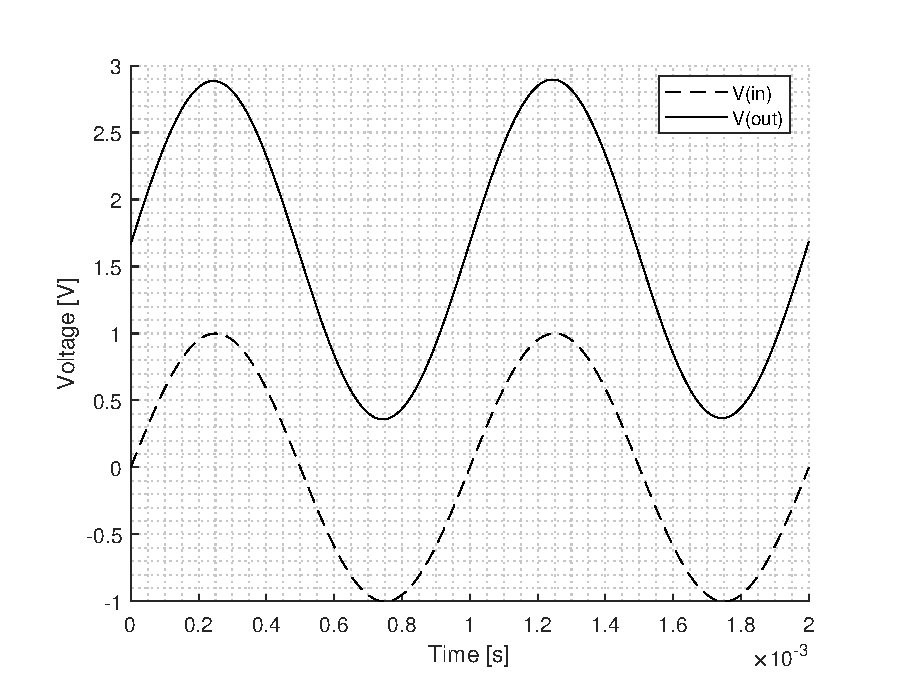
\includegraphics[width=.8\textwidth]{Figures/3_dc_coupler_sim_transient.eps}
	\caption{Transient analysis of DC-Coupling filter circuit}
	\label{fig:3_dccoupler_sim_transient}
\end{figure}

\section{Digital Signal Processor}
In the \gls{dsp} system, the function is to turn a waveform into a humanly readable velocity metric by performing an \gls{fft} of the input signal captured from the output of the active filter of the previous section. Since DSP devices are programmable \gls{dc} devices of typically \qtyrange{3.3}{5}{\volt}, it is vital that the input signal is \gls{dc}-coupled. Since the input signal is relatively low frequency, most \gls{adc} interfaces should be sufficient to capture a frequency window of less than \qty{10}{\kilo\hertz}.
	\chapter{Implementation}
In this chapter, the steps involved in turning a theoretical design into a tangible system will be outlined. Since the synthesis chapter dealt with an explanation of the functions of each module and simulations, with a subsequent evaluation of the outcomes, this chapter will focus on the creation of physical hardware setups and reproducing the desired results using lab experiments. As such, each module will be tested independently to validate its function before a larger, more comprehensive experiment is conducted. All figures in this chapter show measurements performed on physical hardware.
\section{Control System}
\begin{figure}[htbp]
	\centering
	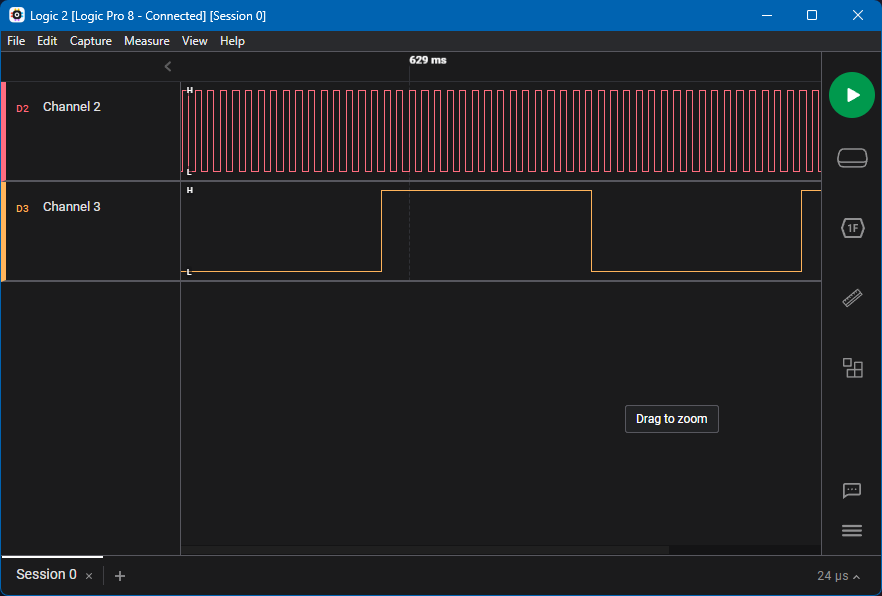
\includegraphics[width=.8\textwidth]{Figures/4_controlsystem_stm32_zephyr.png}
	\caption{STM32 Zephyr RTOS pulser output}
	\label{fig:4_stm32_zephyr_pulser}
\end{figure}
During the initial implementation stage of the control system, a bring-up of the STM32F411RE board and several pulse signals were succesfully generated. In \cref{fig:4_stm32_zephyr_pulser}, two pulse signals can be seen. In Channel 2, \qty{5}{\mega\hertz} ultrasound pulse can be seen. In Channel 3, the \qty{10}{\kilo\hertz} PRF signal can be seen. Unfortunately, soon thereafter it was discovered a limitation of the API in Zephyr is not mature enough developed for power systems such as the half-bridge in the transmitter circuit. In more practical terms, it was not possible to generate two complementary signals with dead-time using the existing Zephyr PWM API. To continue with that solution, a new PWM driver would have to be written from scratch, which is no trivial task. Alternative solutions were investigated. Another option was to use the \gls{hal} provided by the manufacturer of the microcontroller. However, it was decided to try an alternative system known as PYNQ Z1, which is a development board by Agilent. On the PYNQ Z1 board is a Zynq 7000 \gls{soc}. Inside the Zynq 7000 SoC there are both an \gls{fpga} and an Arm based processor. \todo{Write more}

\section{Power Stage}
\begin{figure}[htbp]
	\centering
	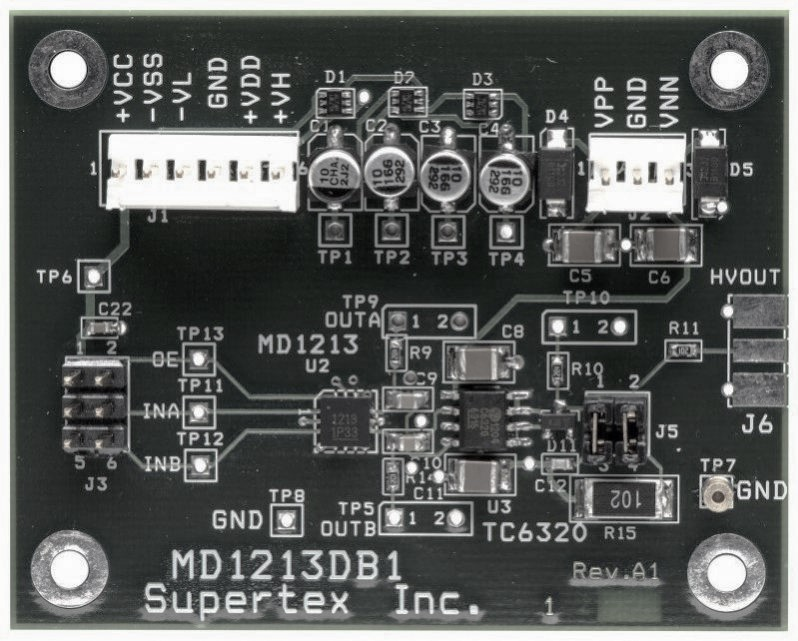
\includegraphics[width=.8\textwidth]{Figures/4_transmitter_pcb_pic.jpg}
	\caption{MD1213DB1 High Speed Pulser}
	\label{fig:4_transmitter_pcb_pic}
\end{figure}
A picture of the power stage PCB can be seen in \cref{fig:4_transmitter_pcb_pic}. An experiment is conducted to validate the function of the power stage. Using the jumpers, the PCB is configured without its onboard load, and a \gls{pzt} transducer is attached with a splitter adapter to connect the other side to an oscilloscope for data acquisition. Seen in \cref{fig:4_transmitter_meas} are actual measured inputs and outputs of the power stage. On the input, there are two complementary \qty{5}{\mega\hertz} signals with varying duty cycle to generate the desired dead time. On the output, we see the rail-to-rail push-pull operation of the \gls{mosfet} half-bridge. The schematic of the transmitter can be found in the appendix in \cref{fig:appendix_md1213db1}. Noticeable noise is observed in the input signal top and base but is negligible for successful operation. Possibly, the noise is due to a cable and adapter setup.
\begin{figure}[htbp]
	\centering
	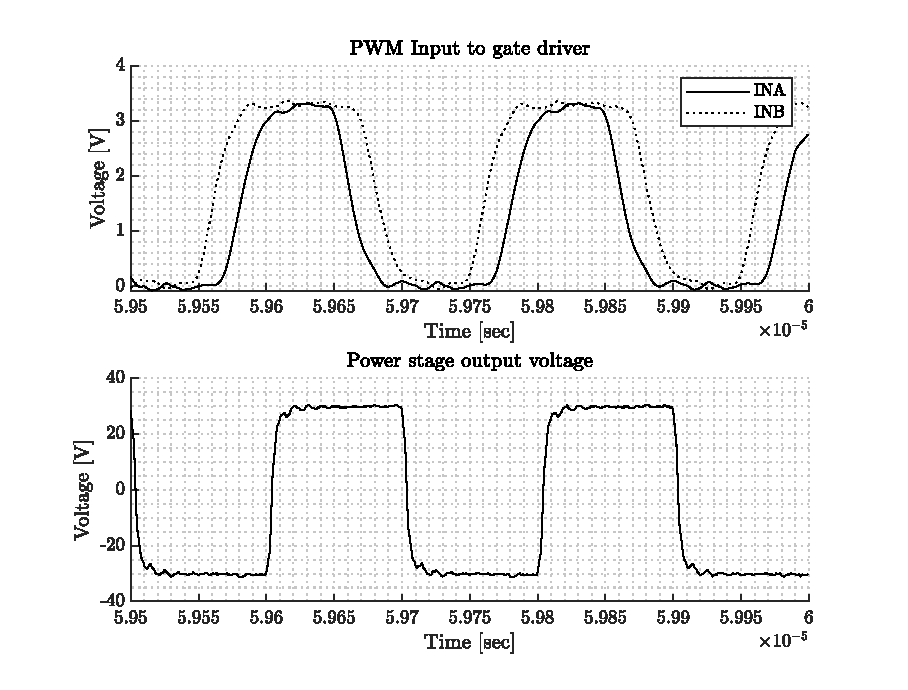
\includegraphics[width=.8\textwidth]{Figures/4_transmitter_pcb_out.eps}
	\caption[Measured input and output of power stage PCB]{Measured input and output of power stage PCB. (Above) Input to gate driver with dead-time (Below) Output of MOSFET half-bridge and the voltage across the load}
	\label{fig:4_transmitter_meas}
\end{figure}
\section{Transmit/Receive Switch}
\begin{figure}[htbp]
	\centering
	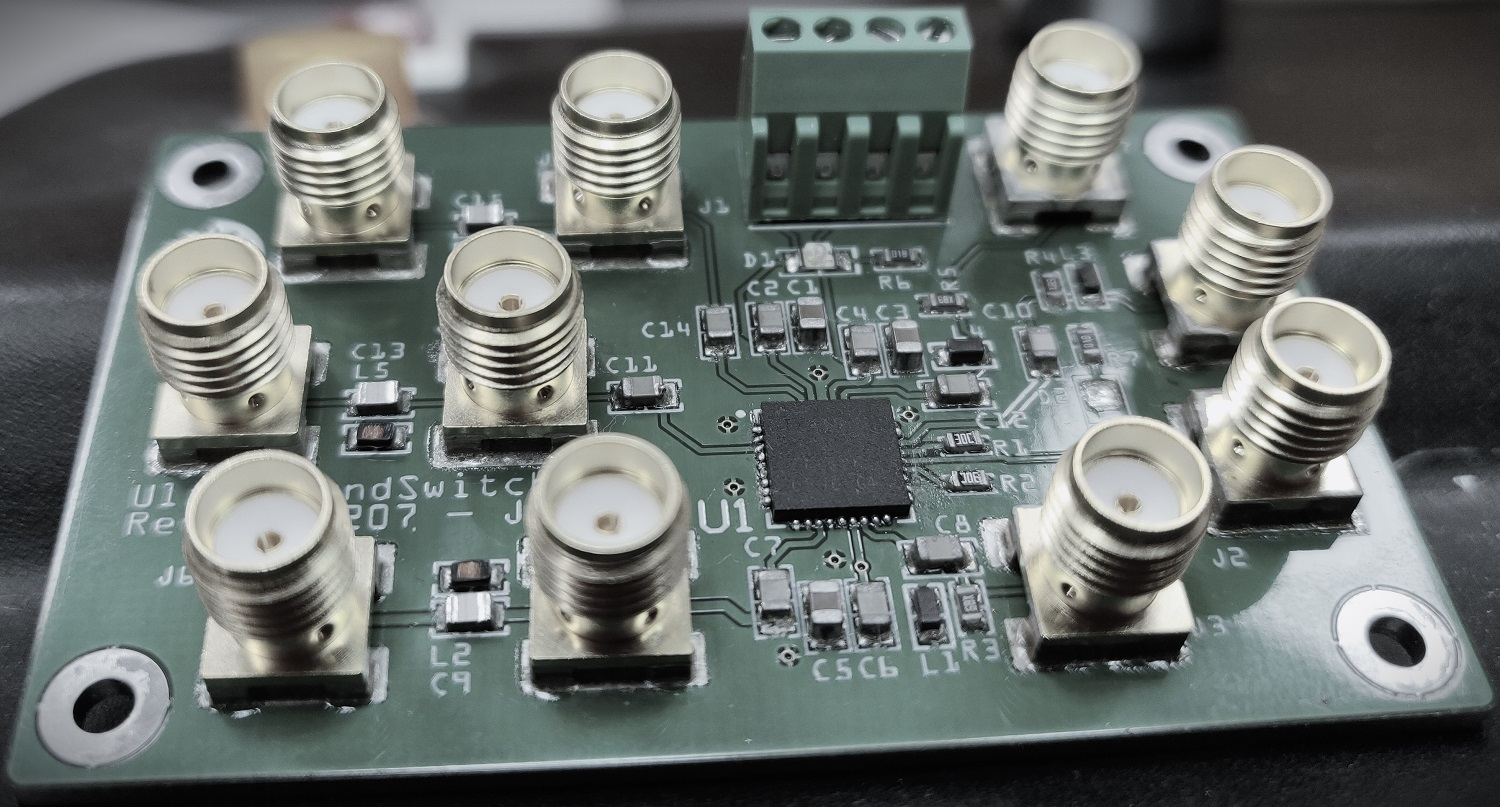
\includegraphics[width=.8\textwidth]{Figures/4_switch_pcb_pic.jpg}
	\caption[Transmit/Receive Switch after assembly]{Transmit/Receive Switch after assembly}
	\label{fig:4_txrx_pcb}
\end{figure}
The entire schematic of the transmit/receive switch can be found in the appendix in \cref{fig:appendix_ultrasoundswitch_a,fig:appendix_ultrasoundswitch_b}. As mentioned in the previous chapter, a PCB layout was made and a batch of 5 was ordered with an accompanying stencil for fast assembly. After the PCBs arrived, the stencil was mounted in the stencil frame and the PCB was aligned for solder paste application. After the solder paste application is completed, all the components are placed on their corresponding footprints and the PCB is placed in the reflow oven. The equipment used in this process is listed in \cref{tab:instruments_solder_work}. The finished assembly can be seen in \cref{fig:4_txrx_pcb}.
\begin{figure}[htbp]
	\centering
	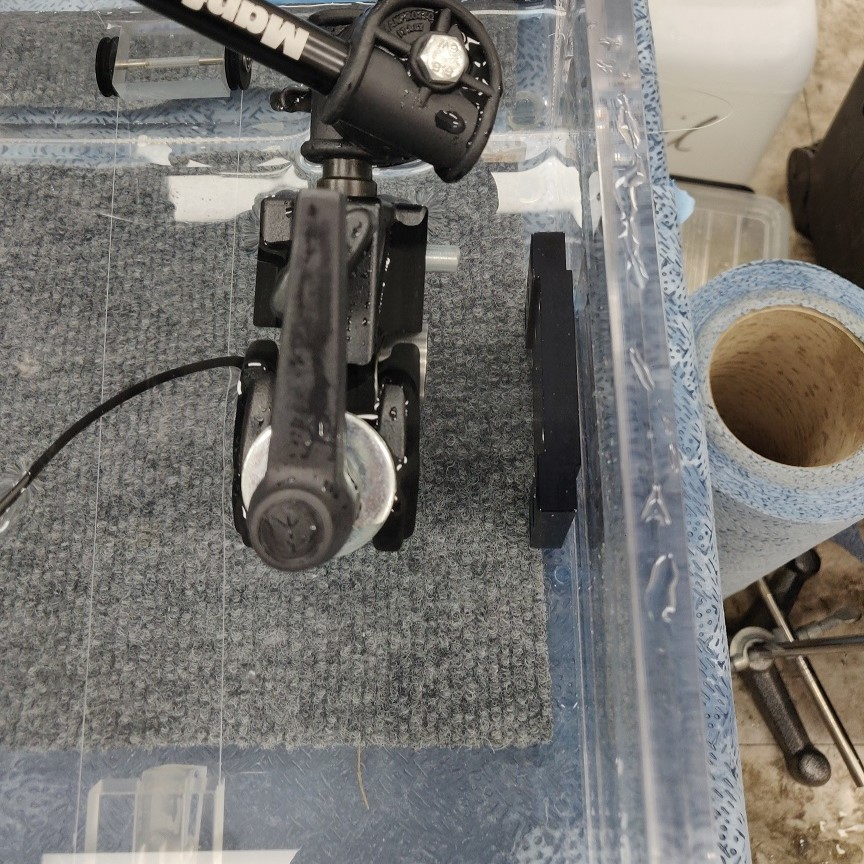
\includegraphics[width=.8\textwidth]{Figures/4_switch_meas_pic.jpg}
	\caption{TX/RX Switch reflection experiment with water tank}
	\label{fig:4_switch_meas_pic}
\end{figure}
For validating the TX/RX switch, an experiment is conducted with a \gls{pzt} transducer, water tank, function generator and an oscilloscope. Using two input signals, $f_{\mathrm{prf}}=\qty{10}{\kilo\hertz}$ switch signal, and $f_{0}=\qty{5}{\mega\hertz}$ burst mode transmit signal, the switch is configured to transmit and receive. A picture of the submerged transducer with a reflector can be seen in \cref{fig:4_switch_meas_pic}. After submerging the transducer in distilled water and measuring on the receiver side of the TX/RX switch, a reflected signal from the tank can be observed in \cref{fig:4_txrx_meas}.
\begin{figure}[htbp]
	\centering
	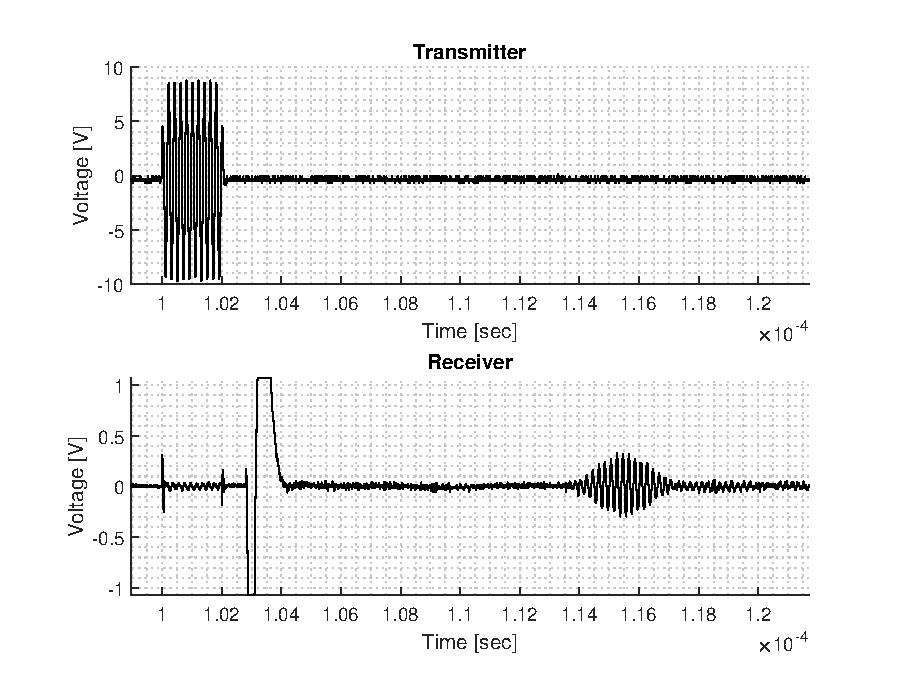
\includegraphics[width=.8\textwidth]{Figures/4_switch_pcb_meas.eps}
	\caption[Measured transmit and receive on Transmit/Receive Switch PCB]{Measured transmit and receive on Transmit/Receive Switch PCB (Above) Measured transmit voltage (Below) Received reflected signal off water tank}
	\label{fig:4_txrx_meas}
\end{figure}
\section{Band-Pass Filter}
As the band-pass filter was described in the previous chapter, it is desired to validate its frequency response to determine if it functions as desired. To obtain the frequency response, a bode plot of the magnitude and phase is measured from \qty{300}{\kilo\hertz} until \qty{20}{\mega\hertz} using a \gls{vna} in a S21 configuration, meaning a measurement of the output in respect to the input. This measurement determines the difference in magnitude and phase of the output in comparison with the input signal. Observed in \cref{fig:4_bpf_measurement} is the frequency response of the band-pass filter measured on a \gls{vna}. It is noted that the pass band frequencies are mostly as expected with \qty{-0.5}{\decibel} frequencies at \qty{1.5}{\mega\hertz} and \qty{7}{\mega\hertz}. Though, the roll-off in the higher stop band appears somewhat lower than in the lower stop band. That would mean that it is plausible that higher frequency noise components are retained in the output than in the lower stop band. For the phase, it seems to have a significant phase delay, going from around \qty{100}{\degree} to \qty{250}{\degree} from the start to the end of the pass band.
\begin{figure}[htbp]
	\centering
	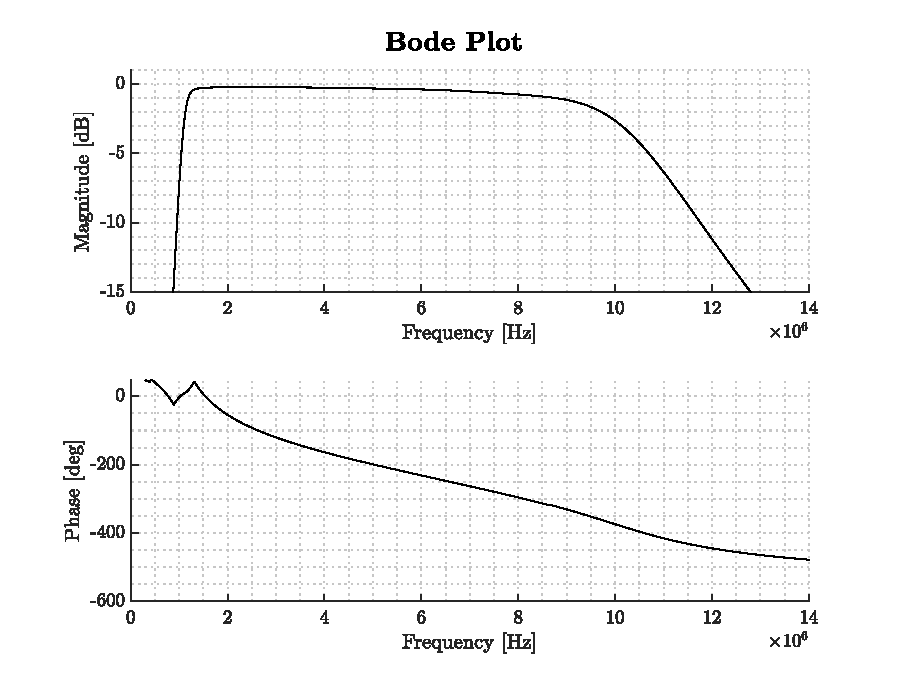
\includegraphics[width=.8\textwidth]{Figures/4_bpf_measurement_vna.eps}
	\caption[Band-pass filter bode plot]{Band-pass Filter bode plot from \qtyrange{0.3}{14}{\mega\hertz} with (above) magnitude and (below) phase}
	\label{fig:4_bpf_measurement}
\end{figure}

\section{Preamplifier}
Before the signal can be demodulated, it must be DC-biased and amplified. This is what the preamplifier is for. For the preamplifier, the circuit is validated using an experiment where a function generator is transmitting a low amplitude sine with ac-coupling and measure the amplified dc-coupled output. Seen in \cref{fig:4_preamp_in} are measurements of the preamplifier circuits showing a \qty{70}{\milli\volt} input signal and a \qty{300}{\milli\volt} output signal with a \qty{2.5}{\volt} DC bias. In this application, however, only the \gls{lna} is used, and the \gls{vga} is bypassed in the hardware preamplifier configuration. The schematic of the preamplifier circuit is part of the demodulation schematic and can be found in the appendix in \cref{fig:appendix_ad8333}.
\begin{figure}[htbp]
	\centering
	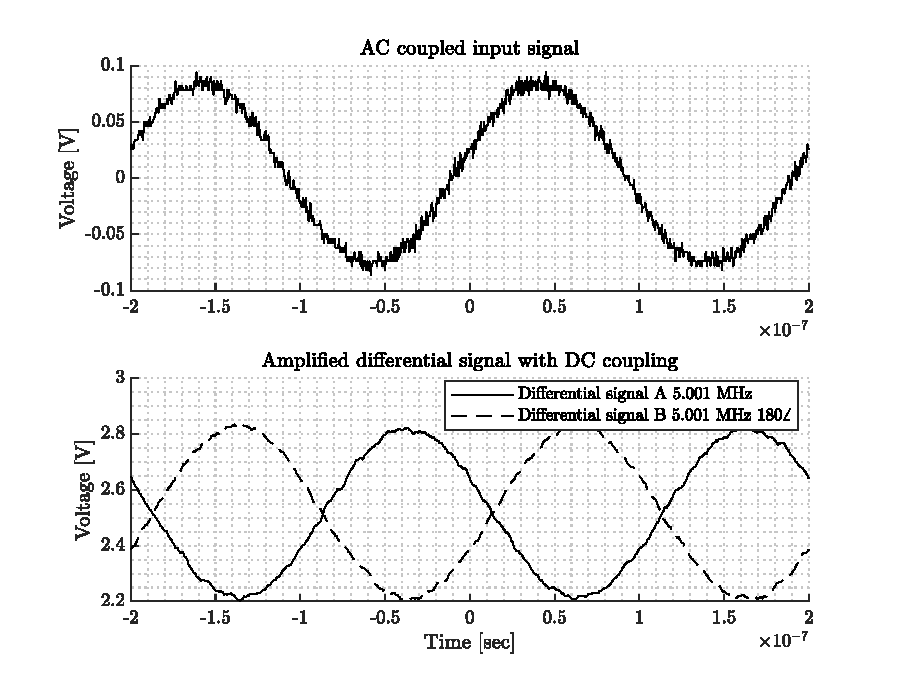
\includegraphics[width=.8\textwidth]{Figures/4_preamplifier_pcb.eps}
	\caption[Measured input and output of preamplifier PCB]{Measured input of preamplifier PCB, (Above) AC coupled input signal with amplitude \qty{1}{\volt} (Below Measured output of preamplifier PCB, Differential signal with DC coupling and $\times \qty{19}{\decibel}$ amplification)}
	\label{fig:4_preamp_in}
\end{figure}
\section{Quadrature Demodulator}
\begin{figure}[htbp]
	\centering
	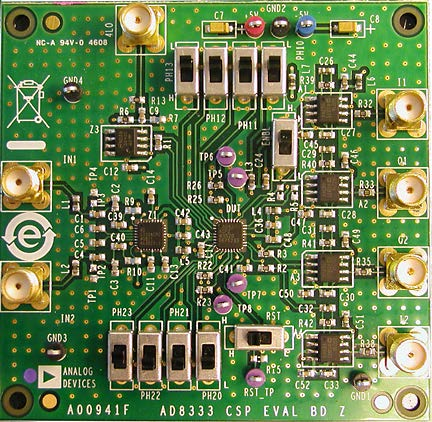
\includegraphics[width=.8\textwidth]{Figures/4_demod_pcb_pic.jpg}
	\caption{Demodulator PCB AD8333-EVALZ}
	\label{fig:4_demod_pcb_pic}
\end{figure}
As described in the previous chapter, the demodulator use an I/Q quadrature demodulation scheme to take two differential RF signals and a quadruple frequency signal, in this case, \qty{5}{\mega\hertz} and \qty{20}{\mega\hertz}, respectively, and determines the frequency difference between the fundamental frequency and the Doppler frequency on the output. Seen in \cref{fig:4_demod_in} are the input signals, differential signals of \qty{5.001}{\mega\hertz} and \qty{20}{\mega\hertz} local oscillator signal. Seen in \cref{fig:4_demod_out} are the differential input signals $A$ and $B$ and the demodulated output signals $I$ and $Q$, where the phase between $I$ and $Q$ denotes the Doppler shift direction, or rather, the direction of flow of the scatterer. It is noted that the differential signal is so high frequency compared to the timescale so there has to be a zoomed in subplot where the waveform is visible to show the waveform. This highlights the significant frequency difference, which is one of the key functions of the demodulator.

\begin{figure}[htbp]
	\centering
	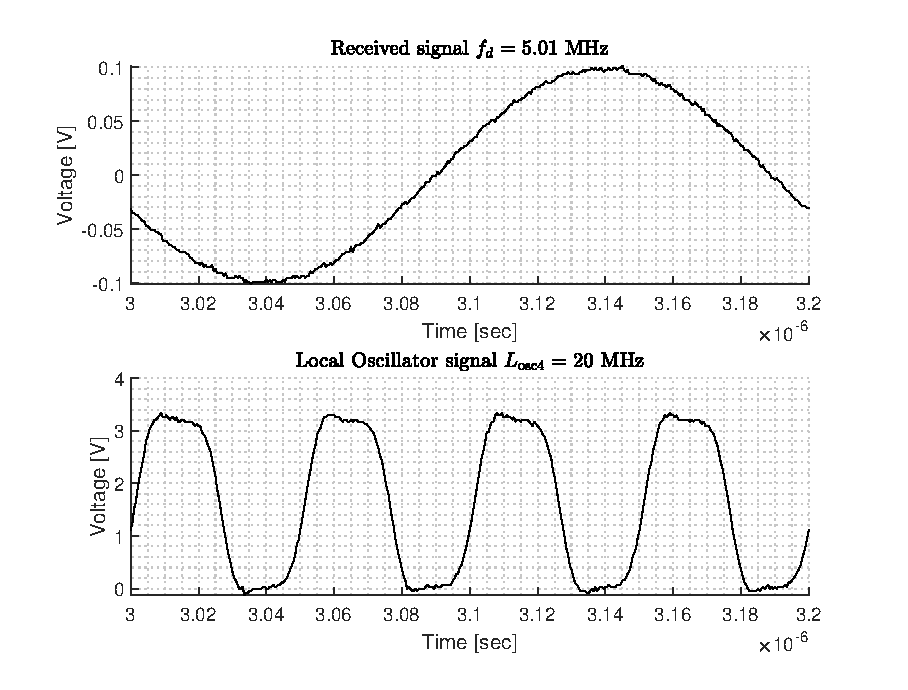
\includegraphics[width=.8\textwidth]{Figures/4_demod_pcb_in.eps}
	\caption[Measured input of demodulator PCB]{Measured input of demodulator PCB (Above) Input from received signal (Below) Input from local oscillator ($f_{0}\cdot4$)}
	\label{fig:4_demod_in}
\end{figure}
\begin{figure}[htbp]
	\centering
	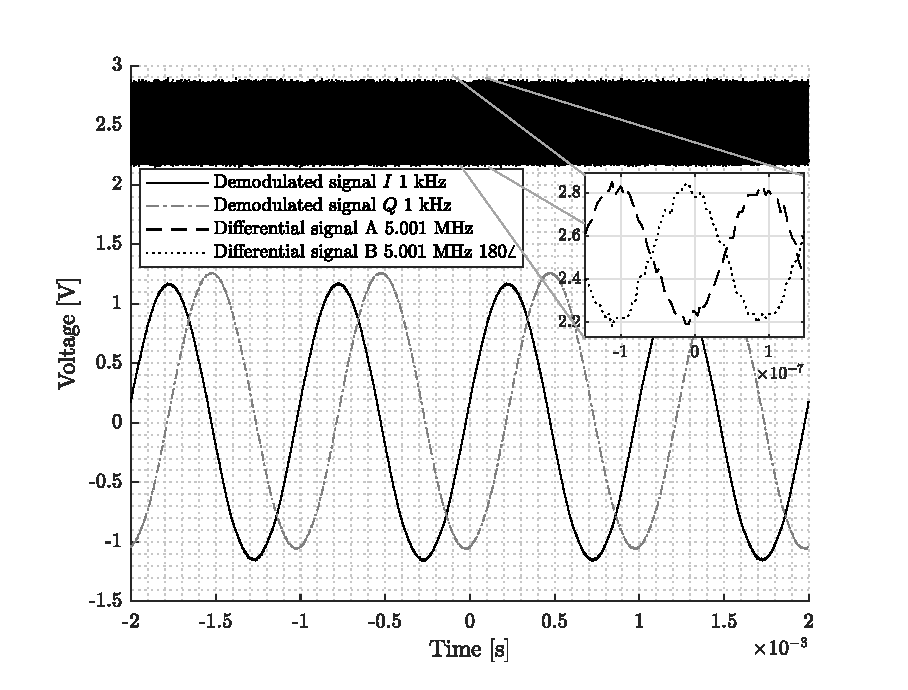
\includegraphics[width=.8\textwidth]{Figures/4_demod_pcb_out.eps}
	\caption[Measured output of demodulator PCB]{Measured output of demodulator PCB}
	\label{fig:4_demod_out}
\end{figure}
The entire schematic of the demodulator can be found in the appendix in \cref{fig:appendix_ad8333}.
\section{Sample and Hold}
After each demodulated burst is sampled, between each sample line pulse repetition it is desired to hold the voltage, so the analogue-to-digital conversion that may be running asynchronously does not sample zero-values between the bursts. Therefore, an experiment is conducted with the sample-and-hold amplifier to verify the functionality. A low-frequency I-Q simulated signal is created from the function generator with a sample gating pulse train to control the sample-and-hold function. Seen in \cref{fig:4_sample_hold_pcb} is the measured inputs and outputs of the circuit during the experiment. Above is the I-Q input and in the middle is the sample gating, and below is the output signal. On the output signal, it is noted the corresponding voltage transients for every pulse in the gate input.
\begin{figure}[htbp]
	\centering
	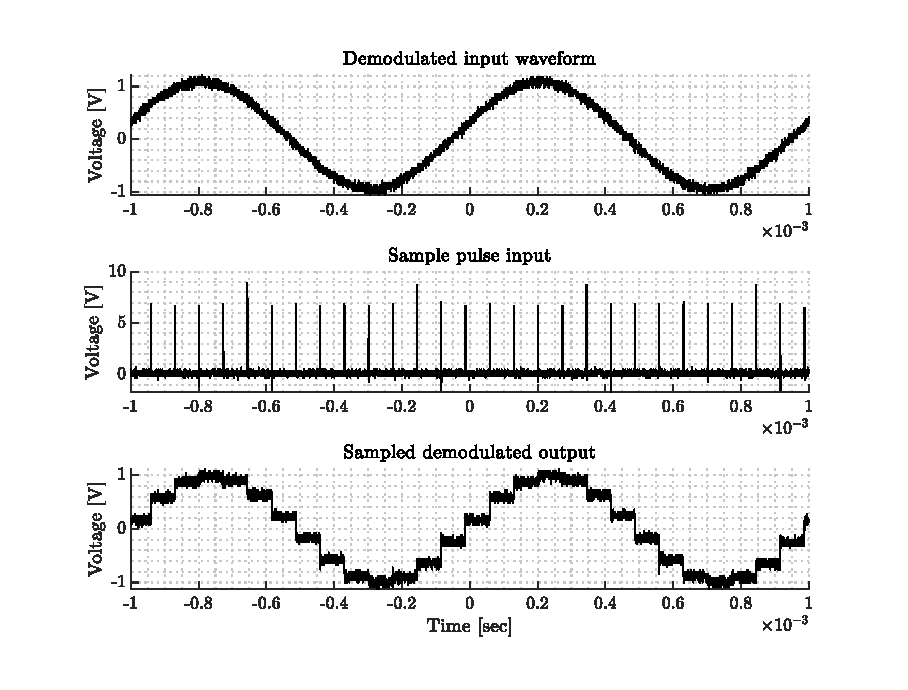
\includegraphics[width=.8\textwidth]{Figures/4_sampler_pcb.eps}
	\caption{Measured input and output of Sample and Hold amplifier}
	\label{fig:4_sample_hold_pcb}
\end{figure}

\section{Pulse-Repetition and Wall Filter}
\section{Digital Signal Processor}


%\begin{figure}[H]
%	\centering
%	\begin{circuitikz}[american voltages]
%		\draw
%		(0,0) to [short, *-] (6,0)
%		to [V, l_=$\mathrm{j}{\omega}_m \underline{\psi}^s_R$] (6,2)
%		to [R, l_=$R_R$] (6,4)
%		to [short, i_=$\underline{i}^s_R$] (5,4)
%		(0,0) to [open, v^>=$\underline{u}^s_s$] (0,4)
%		to [short, *- ,i=$\underline{i}^s_s$] (1,4)
%		to [R, l=$R_s$] (3,4)
%		to [L, l=$L_{\sigma}$] (5,4)
%		to [short, i_=$\underline{i}^s_M$] (5,3)
%		to [L, l_=$L_M$] (5,0);
%	\end{circuitikz}
%	\caption{The nodes short, V, R and L are presented here, but there a lot more}
%	\label{fig:circuitikz}
%\end{figure}
%
%\section{Listings (code)}
%
%\Cref{lst:helloworld} is a nicely formatted block of code. A listing will automatically continue on the next page if it encounters a page break. Many different programming languages can be highlighted. Check the \texttt{listings} package documentation for a list of supported programming languages.

%\begin{listing}[htbp]
%\begin{mintedc}
%#include <stdio.h>
%int main()
%{
%	printf("Hello, World!"); /*printf() outputs the quoted string*/
%	if (n == 0 || n == 1){
%		return n;
%	}
%	j = 0;
%	for (i = 0; i < n-1; i++){
%		if (arr[i] != arr[i+1]){
%			arr[j] = arr[i];
%			j++;
%		}
%	}
%	arr[j++] = arr[n-1];
%	return 0;
%}
%\end{mintedc}
%	\caption{Hello world in C}
%	\label{lst:helloworld}
%\end{listing}




	\chapter{Analysis}
In this chapter every subcomponent will be part of an experiment in isolation to validate their function. Also, various test setups will be discussed for the purpose of making multi-module experiments in the AFE and control system to evaluate their performance and compatibility. As such, each module will be tested independently to validate its function before a larger, more comprehensive experiment is conducted. All figures in this chapter show measurements performed on physical hardware.

\section{Module Testing}
\subsection{Control System}
First, a bitstream was generated with a Pwm generator and AXI interconnect registers. An AXI interconnect register is a method to create GPIO interfaces between the logical processor and the Arm processor on the Zynq 7000 SoC using registers that temporarily store GPIO data in the bitstream overlay. A block diagram of the overlay can be seen in \cref{fig:app_fpga_block_diagram} and the JupyterLab notebook can be seen in \cref{fig:app_jupyter_notebook}.

\begin{figure}[htbp]
	\centering
	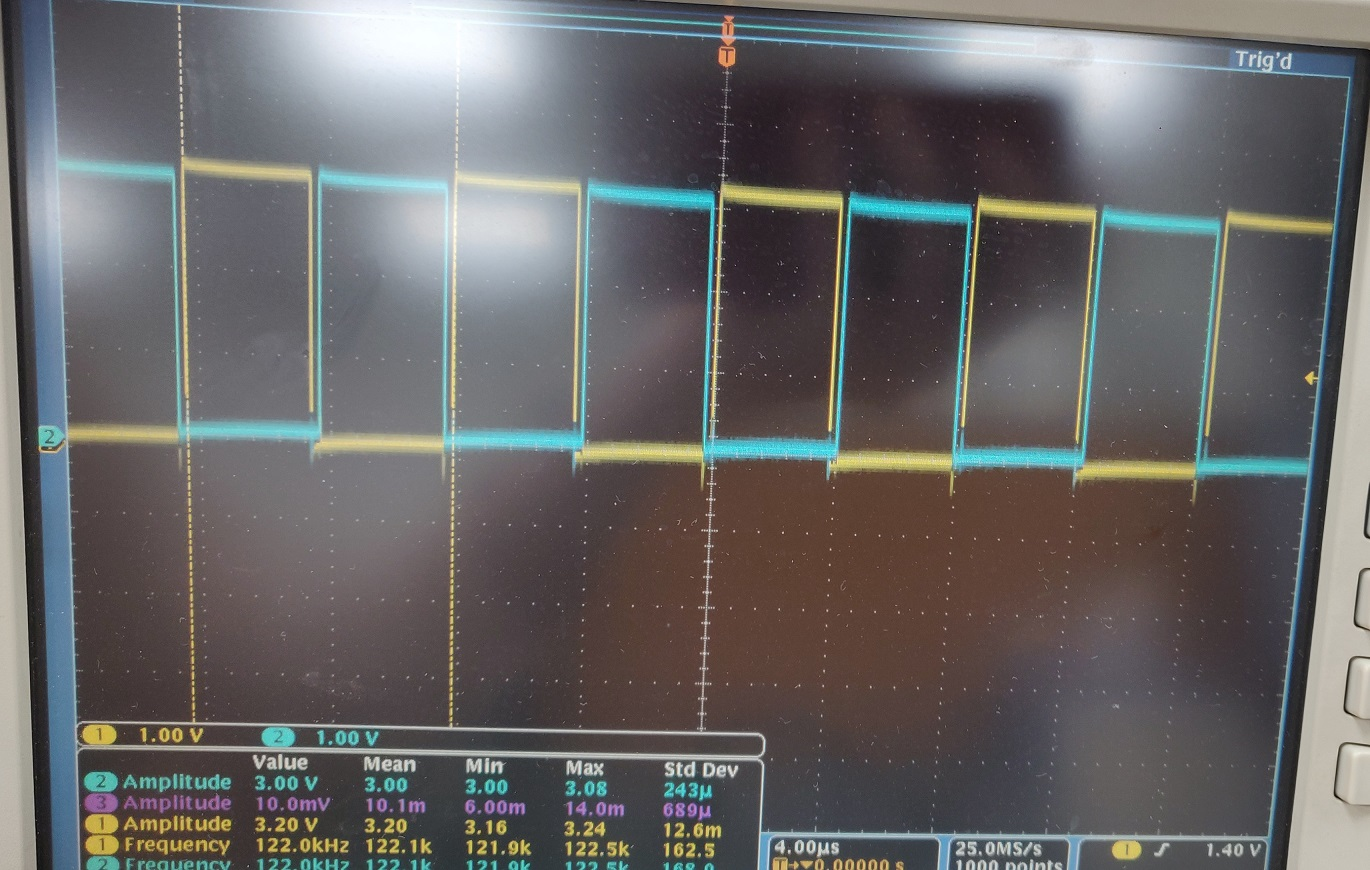
\includegraphics[width=.8\textwidth]{Figures/4_controlsystem_fpga_pwm.png}
	\caption{Complementary PWM output with Pynq Z1 FPGA and JupyterLab notebook}
	\label{fig:4_controlsystem_fpga_pwm}
\end{figure}
A preliminary implementation was implemented in Vivado and JupyterLab for a continuous complementary PWM controller. The resulting measurement can be seen in \cref{fig:4_controlsystem_fpga_pwm} before a clock configuration, which means the frequency corresponded to an arbitrary temporary pulse frequency of \qty{122}{\kilo\hertz}. As the initial test proved successful, the continued development and maturation of the pulser enabled a complete signal generator for the ultrasound pulse generator.

\begin{figure}[htbp]
	\centering
	\includegraphics[width=\linewidth]{Figures/5_controlsystem_fpga_pulser_logic.eps}
	\caption{Captured timing diagram of the control system pulser}
	\label{fig:5_controlsystem_pulser_logic}
\end{figure}
Seen in \cref{fig:5_controlsystem_pulser_logic} are the measured signals from the pulse generator showing the various timings of each signal captured with a Salae Logic Analyzer Pro 8.

\subsection{Power Stage}
Seen in \cref{fig:4_transmitter_meas} are actual measured inputs and outputs of the power stage. On the input, there are two complementary \qty{5}{\mega\hertz} signals with varying duty cycle to generate the desired dead time. On the output, we see the rail-to-rail push-pull operation of the \gls{mosfet} half-bridge. The schematic of the transmitter can be found in the appendix in \cref{fig:appendix_md1213db1}. Noticeable noise is observed in the input signal top and base but is negligible for successful operation. Possibly, the noise is due to a cable and adapter setup.
\begin{figure}[htbp]
	\centering
	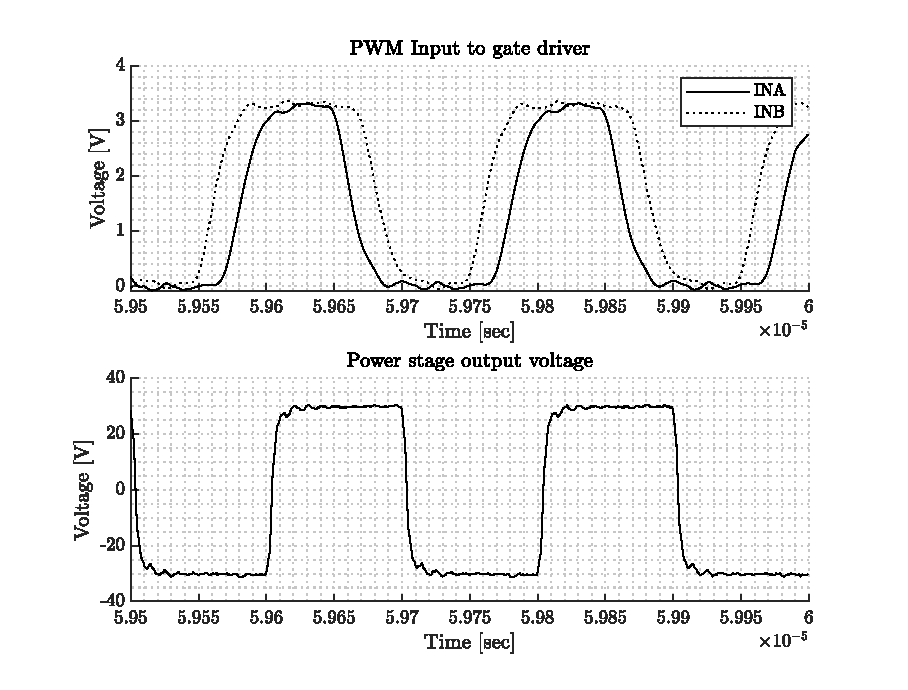
\includegraphics[width=.8\textwidth]{Figures/4_transmitter_pcb_out.eps}
	\caption[Measured input and output of power stage PCB]{Measured input and output of power stage PCB. (Above) Input to gate driver with dead-time (Below) Output of MOSFET half-bridge and the voltage across the load}
	\label{fig:4_transmitter_meas}
\end{figure}

\subsection{Transmit/Receive Switch}
\begin{figure}[htbp]
	\centering
	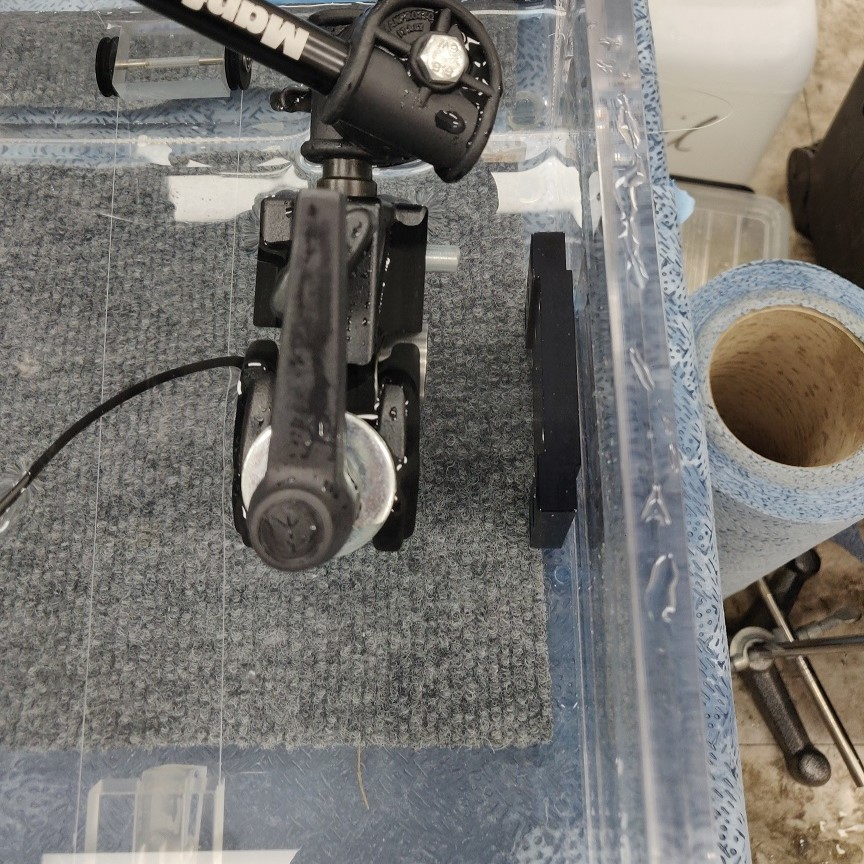
\includegraphics[width=.8\textwidth]{Figures/4_switch_meas_pic.jpg}
	\caption{TX/RX Switch reflection experiment with water tank}
	\label{fig:4_switch_meas_pic}
\end{figure}
For validating the TX/RX switch, an experiment is conducted with a \gls{pzt} transducer, water tank, function generator and an oscilloscope. Using two input signals, $f_{\mathrm{prf}}=\qty{10}{\kilo\hertz}$ switch signal, and $f_{0}=\qty{5}{\mega\hertz}$ burst mode transmit signal, the switch is configured to transmit and receive. A picture of the submerged transducer with a reflector can be seen in \cref{fig:4_switch_meas_pic}. After submerging the transducer in distilled water and measuring on the receiver side of the TX/RX switch, a reflected signal from the tank can be observed in \cref{fig:4_txrx_meas}.
\begin{figure}[htbp]
	\centering
	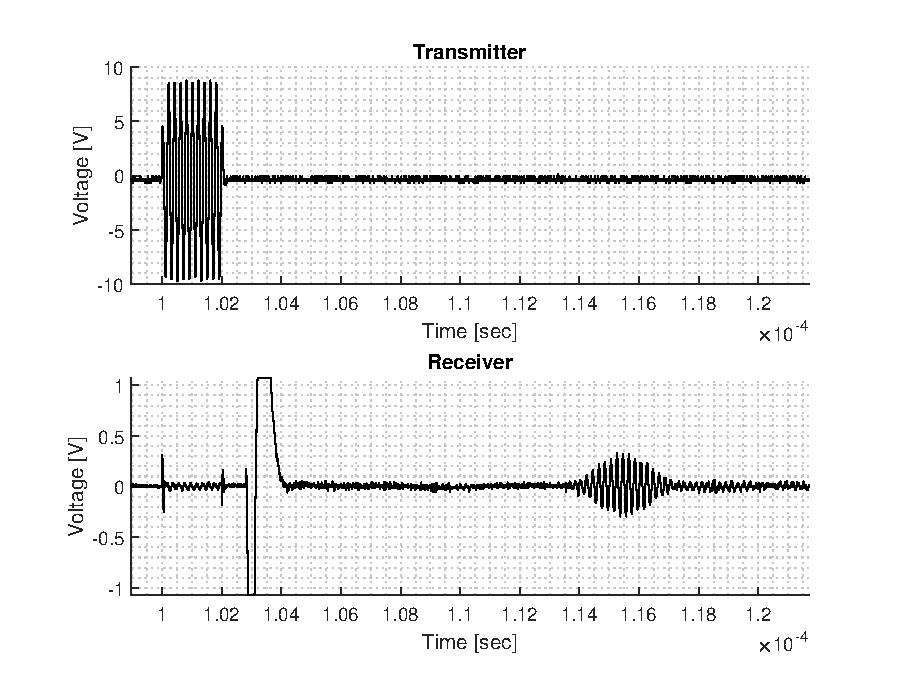
\includegraphics[width=.8\textwidth]{Figures/4_switch_pcb_meas.eps}
	\caption[Measured transmit and receive on Transmit/Receive Switch PCB]{Measured transmit and receive on Transmit/Receive Switch PCB (Above) Measured transmit voltage (Below) Received reflected signal off water tank}
	\label{fig:4_txrx_meas}
\end{figure}

\subsection{Band-pass Filter}
it is desired to validate its frequency response to determine if it functions as desired. To obtain the frequency response, a bode plot of the magnitude and phase is measured from \qty{300}{\kilo\hertz} until \qty{20}{\mega\hertz} using a \gls{vna} in a S21 configuration, meaning a measurement of the output in respect to the input. This measurement determines the difference in magnitude and phase of the output in comparison with the input signal. Observed in \cref{fig:4_bpf_measurement} is the frequency response of the band-pass filter measured on a \gls{vna}. It is noted that the pass band frequencies are mostly as expected with \qty{-0.5}{\decibel} frequencies at \qty{1.5}{\mega\hertz} and \qty{7}{\mega\hertz}. Though, the roll-off in the higher stop band appears somewhat lower than in the lower stop band. That would mean that it is plausible that higher frequency noise components are retained in the output than in the lower stop band. For the phase, it seems to have a significant phase delay, going from around \qty{100}{\degree} to \qty{250}{\degree} from the start to the end of the pass band.
\begin{figure}[htbp]
	\centering
	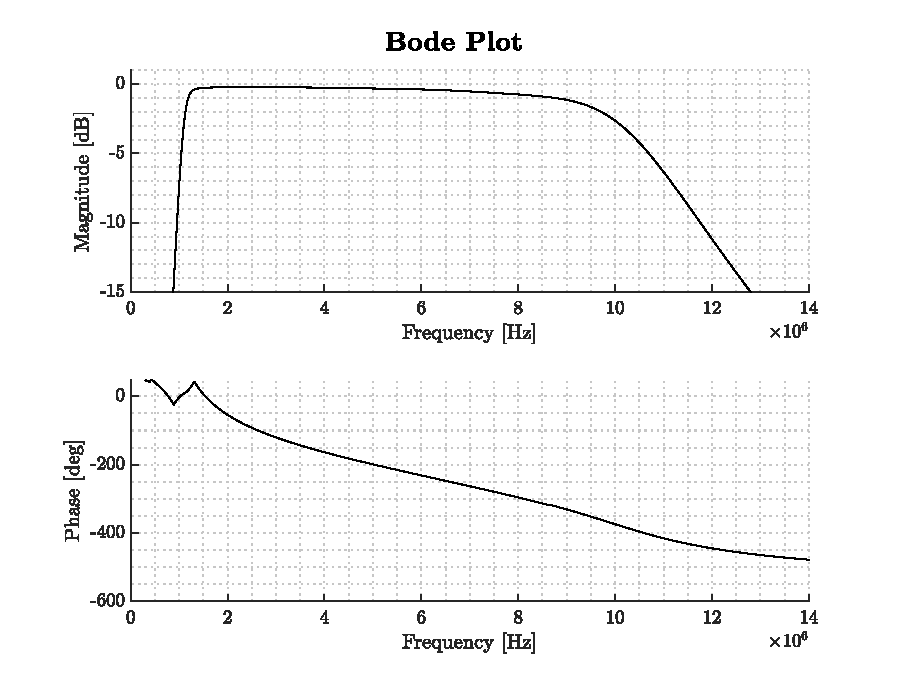
\includegraphics[width=.8\textwidth]{Figures/4_bpf_measurement_vna.eps}
	\caption[Band-pass filter bode plot]{Band-pass Filter bode plot from \qtyrange{0.3}{14}{\mega\hertz} with (above) magnitude and (below) phase}
	\label{fig:4_bpf_measurement}
\end{figure}

\subsection{Preamplifier}
Seen in \cref{fig:4_preamp_in} are measurements of the preamplifier circuits showing a \qty{70}{\milli\volt} input signal and a \qty{300}{\milli\volt} output signal with a \qty{2.5}{\volt} DC bias. In this application, however, only the \gls{lna} is used, and the \gls{vga} is bypassed in the hardware preamplifier configuration. The schematic of the preamplifier circuit is part of the demodulation schematic and can be found in the appendix in \cref{fig:appendix_ad8333}.
\begin{figure}[htbp]
	\centering
	\includegraphics[width=.8\textwidth]{Figures/4_preamplifier_pcb.eps}
	\caption[Measured input and output of preamplifier PCB]{Measured input of preamplifier PCB, (Above) AC coupled input signal with amplitude \qty{1}{\volt} (Below Measured output of preamplifier PCB, Differential signal with DC coupling and $\times \qty{19}{\decibel}$ amplification)}
	\label{fig:4_preamp_in}
\end{figure}

\subsection{Demodulator}
An experiment is conducted with the sample-and-hold amplifier to verify the functionality. A low-frequency I-Q simulated signal is created from the function generator with a sample gating pulse train to control the sample-and-hold function. Seen in \cref{fig:4_demod_in} are the input signals, differential signals of \qty{5.001}{\mega\hertz} and \qty{20}{\mega\hertz} local oscillator signal. Seen in \cref{fig:4_demod_out} are the differential input signals $A$ and $B$ and the demodulated output signals $I$ and $Q$, where the phase between $I$ and $Q$ denotes the Doppler shift direction, or rather, the direction of flow of the scatterer. It is noted that the differential signal is so high frequency compared to the timescale so there has to be a zoomed in subplot where the waveform is visible to show the waveform. This highlights the observation of the Doppler shift being pushed down in frequency, which is one of the key functions of the demodulator in this system.

\begin{figure}[htbp]
	\centering
	\includegraphics[width=.8\textwidth]{Figures/4_demod_pcb_in.eps}
	\caption[Measured input of demodulator PCB]{Measured input of demodulator PCB (Above) Input from received signal (Below) Input from local oscillator ($f_{0}\cdot4$)}
	\label{fig:4_demod_in}
\end{figure}
\begin{figure}[htbp]
	\centering
	\includegraphics[width=.8\textwidth]{Figures/4_demod_pcb_out.eps}
	\caption[Measured output of demodulator PCB]{Measured output of demodulator PCB}
	\label{fig:4_demod_out}
\end{figure}

\subsection{Sample and Hold Amplifier}
Seen in \cref{fig:4_sample_hold_pcb} is the measured inputs and outputs of the circuit during the experiment. Above is the I-Q input and in the middle is the sample gating, and below is the output signal. On the output signal, it is noted the corresponding voltage transients for every pulse in the gate input.
\begin{figure}[htbp]
	\centering
	\includegraphics[width=.8\textwidth]{Figures/4_sampler_pcb.eps}
	\caption{Measured input and output of Sample and Hold amplifier}
	\label{fig:4_sample_hold_pcb}
\end{figure}

\subsection{Active Filter, DC Coupler}
\begin{figure}
	\centering
	\includegraphics[width=.8\textwidth]{Figures/5_dccoupler_filter_measurement.eps}
	\caption{Measured input and output of Active filter and DC Coupler}
	\label{fig:5_dccoupler_measured}
\end{figure}
Seen in \cref{fig:5_dccoupler_measured} is the measured input and output of the DC coupler and active filter. The dashed line is the \gls{ac} coupled input signal with \qty{1}{\volt} amplitude and the solid line is the amplified \gls{dc} coupled output signal.

\section{Pulse Generator and Power Stage}
Using the pulse generator and the power stage, an experiment is performed where the complementary PWM signals are generated and output to the gate driver of the power stage. In turn, the gate driver will drive the MOSFET pair and output a high-power output than the pulse generator can supply on its own through its \gls{gpio}.

\begin{figure}[htbp]
	\centering
	\includegraphics[width=.8\textwidth]{Figures/5_controlsystem_fpga_pwm.png}
	\caption{Complementary PWM output from the pulse generator and bipolar high power pulses}
	\label{fig:5_pulse_generator_experiment}
\end{figure}

Seen in \cref{fig:5_pulse_generator_experiment} are the measurements obtained from the pulse generator and power stage experiment. The measurements show the ability of the Pynq Z1 as a pulse generator is functioning as expected. As the power stage half-bridge is rail-to-rail, the output pulse voltages depend on the power supply voltage. In this case, the experiment is using a \qty{30}{\volt} maximum \gls{dcps}, and the output peak pulse voltages are $\pm \qty{30}{\volt}$. However, the power stage itself is specified for operating voltages up to $\pm \qty{100}{\volt}$.

\section{Doppler String Phantom Experiment}
The CIRS A043 Doppler String Phantom is a device used to evaluate the performance of Doppler ultrasound imaging systems. The phantom consists of a set of strings that move in a controlled manner when exposed to ultrasound waves. The strings are made of nylon monofilament and are arranged in a parallel array.

When the phantom is scanned with a Doppler ultrasound probe, the strings vibrate in response to the sound waves, producing a Doppler signal. The phantom includes a set of control strings that vibrate at a known frequency, allowing the user to calibrate the system and determine its accuracy. The string is driven by a motor that can be programmed to move at different speeds and directions, and it is also designed to create turbulence, which mimics the flow of blood in diseased vessels.

The phantom also includes a set of strings that move in a complex, non-linear pattern, simulating blood flow in vessels with turbulent flow. This allows the user to test the system's ability to accurately detect and measure turbulent blood flow, which is an important diagnostic feature for conditions such as stenosis or arterial occlusion.

By evaluating the system's performance on the known frequencies of the control strings and the complex patterns of the turbulence strings, the user can assess the accuracy and reliability of the Doppler ultrasound system. The CIRS A043 Doppler String Phantom is widely used in research, development, and quality assurance of Doppler ultrasound equipment.
\begin{figure}[htbp]
	\centering
	\includegraphics[width=.8\textwidth]{Figures/5_cirs_043a_image.jpg}
	\caption[CIRS Model 043A Doppler String Phantom]{CIRS Model 043A Doppler String Phantom with (left) motor controller and (right) tank and string loop}
\end{figure}

\begin{figure}[htbp]
	\centering
	\includegraphics[width=.8\textwidth]{Figures/5_doppler_string_phantom_experiment.pdf}
	\caption{Doppler String Phantom experiment diagram (not to scale)}
	\label{fig:5_doppler_string_experiment}
\end{figure}

	\chapter{Conclusion}
In conclusion, this project has successfully gone through thorough research, data collection, and analysis, and have obtained a comprehensive understanding of the subject matter. Through a literature review, key gaps in the research have been identified. This formed the basis of a design approach to the ultrasound system that was followed throughout the project. This project aimed to design, build, and test an ultrasound system for blood velocity estimation that can be miniaturised. The implementation of all the sub-components in the system was simulated and/or tested thoroughly to verify the function. Moreover, some of the combined testing revealed some implementation changes necessary in the power stage output. Despite the numerous achievements and contributions made throughout this project, it is important to acknowledge its limitations. Factors such as time constraints, limited resources, and external factors beyond our control may have impacted the scope and depth of our study. However, the findings and insights presented in this report should provide a solid foundation for future research and further exploration of the topic. Due to time limitations, experiments were focused on module testing each part of the system independently. It is therefore difficult to compare it with prior research directly. The system was designed around a control system based on the Zynq 7020 SoC, which contains both the configured ultrasound pulser logic controller and the Python-based programmable interface. The transmitter, which includes the ultrasound pulser and the power stage, was tested with the switch, and while the transmitting was successful, a received reflected signal could not be found. It is believed that the received switch was sinking into the on-board load of the power stage.  On the receiver, which includes the bandpass filter, preamplifier, quadrature demodulator, sample and hold circuit, and active filter, were also verified functioning as intended in isolated experiments. The implementation of the analogue frontend can result in a more compact commercial product. However, more work is required before a working single-device prototype can be build and evaluated.
\section{Future Work}
The system was fully validated, although in module testing. TThe absence of eflected signals, when using the  power stage, should be further investigated. In the future, it is desired to perform a complete system test and evaluate the performance using the physiological simulator. After a successful experiment, a single PCB layout can be completed from the CAD work already done for the documentation in Altium Designer. Another future work would be further implementing a continuous data acquisition with a spectral image, thus fully displaying the sonographic data in the DSP. 
	%%
	%% 참고문헌 시작
	%% bibliography
	%% It can be changed but should include sufficient information.
%	\begin{thebibliography}{00}
%
%		\bibitem{FD1} 박상우, \underline{동시 송수신 안테나를 두 개 쓰는 협력 인지 무선통신망에 알맞은 전 이중 통신}, 한국과학기술원 석사 학위 논문, 2016.
%
%		\bibitem{RVP1} 송익호, 박철훈, 김광순, 박소령, \underline{확률변수와 확률과정}, 자유아카데미, 2014.
%
%		\bibitem{ML1} 송익호, 안태훈, 민황기, \underline{인지 무선에서의 광대역 주파수 검출 방법 및 장치}, 특허등록번호 10-1494966, 2015년 2월 12일.
%
%		\bibitem{SOCA1} 호우위시, 이원주, 이승원, 안태훈, 이선영, 민황기, 송익호, “선형 판별 분석에서 부류안 분산 행렬의 영 공간 재공식화,” \underline{한국통신학회 2012년도 추계종합학술발표회}, 대한민국 고려대학교, 242-243쪽, 2012년 11월.
%
%		\bibitem{EF1} 민황기, 안태훈, 이승원, 이성로, 송익호, “비간섭 전력 부하 감시용 고차 적률 특징을 갖는 전력 신호 인식,” \underline{한국통신학회논문지}, 제39C권, 제7호, 608-614쪽, 2014년 7월.
%
%
%
%		\bibitem{FD2} S. Park, \textit{Full-Duplex Communication for Cooperative Cognitive Radio Networks with Two Simultaneous Transmit and Receive Antennas}, Master Thesis, Korea Adv. Inst. Science, Techn., Daejeon, Republic of Korea, 2016.
%
%		\bibitem{RVP2}  I. Song, J. Bae, and S. Y. Kim, \textit{Advanced Theory of Signal Detection: Weak Signal Detection in Generalized Observations}, Springer-Verlag, 2002.
%
%		\bibitem{ML2} I. Song, T. An, and J. Oh, \textit{Near ML decoding method based on metric-first search and branch length threshold,} registration no. US 8018828 B2, Sep. 13, 2011, USA.
%
%		\bibitem{SOCA2} H.-K. Min, T. An, S. Lee, and I. Song, “Non-intrusive appliance load monitoring with feature extraction from higher order moments,” in \textit{Proc. 6th IEEE Int. Conf. Service Oriented Computing, Appl.,} Kauai, HI, USA, pp. 348-350, Dec. 2013.
%
%		\bibitem{EF2} I. Song and S. Lee, “Explicit formulae for product moments of multivariate Gaussian random variables,” \textit{Statistics, Probability Lett.,} vol. 100, pp. 27-34, May 2015.
%
%
%	\end{thebibliography}
%
%
	\printbibliography[heading=bibintoc,title={Bibliography}]
	%%
	%% 감사의 글 시작
	%% Acknowledgement
	%%
	% @command acknowledgement 감사의글
	% @options [1 | 2 | 3 |4 ]
	% - 1 : 본문과 감사의 글이 둘 다 한글일 때  | 2 : 본문은 한글인데 감사의 글이 영어일 때 | 3 :  본문과 감사의 글이 둘 다 영어일 때  | 4 : 본문은 영어인데 감사의 글이 % 한글일 때
	%% It is optional.

	\acknowledgment[4]
%	언제나 저를 바른 길로 이끌어 주시는 송익호 교수님께 큰 고마움을 느낍니다.
%	끝으로 오늘의 제가 있을 수 있도록 사랑으로 키워 주신 가족들에게 감사드립니다.
%	저의 이 작은 결실이 그분들께 조금이나마 보답이 되기를 바랍니다.

	%%
	%% 약력 시작
	%% Curriculum Vitae
	%%
	% @command curriculumvitae 이력서
	% @options [1 | 2 | 3 |4 ]
	% - 1 : 본문과 약력이 둘 다 한글일 때  | 2 : 본문은 한글인데 약력이 영어일 때 | 3 :  본문과 약력이 둘 다 영어일 때  | 4 : 본문은 영어인데 약력이 한글일 때
	%% It is optional and you can change form of this in the class file if you want.
	\curriculumvitae[4]

	% @environment personaldata 개인정보
	% @command     name         이름
	%              dateofbirth  생년월일
	%              birthplace   출생지
	%              domicile     본적지
	%              address      주소지
	%              email        E-mail 주소
	% - 위 6개의 기본 필드 중에 이력서에 적고 싶은 정보를 입력
	% input data only you want
	\begin{personaldata}
		\name       {힌릭스 예폐}
		\dateofbirth{1991}{07}{22}
		\birthplace {Aarhus}
		\address    {}
	\end{personaldata}

	% @environment education 학력
	% @options [default: (none)] - 수학기간을 입력
	\begin{education}
		\item[2008. 3.\ --\ 2010. 2.] 고등학교 (2년 수료)
		\item[2010. 2.\ --\ 2014. 2.] 한국과학기술원 물리학과 (학사)
		\item[2014. 3.\ --\ 2016. 2.] 한국과학기술원 전기및전자공학부 (석사)
	\end{education}

	% @environment career 경력
	% @options [default: (none)] - 해당기간을 입력
	\begin{career}
		\item[2015. 3.\ --\ 2016. 2.] 한국과학기술원 전기및전자공학부 조교
	\end{career}

	% @environment activity 학회활동
	% @options [default: (none)] - 활동내용을 입력
	%%    \begin{activity}
		%%        \item J. Choi, \textbf{Yong-Hyun Kim}, K.J. Chang, and D. Tomanek,
		%%             \textit{Occurrence of itinerant ferromagnetism in C/BN superlattice
			%%             nanotubes}, 5th Asian Workshop on First-Principles Electronic
		%%             Structure Calculations, Seoul (Korea), October., 2002.
		%%    \end{activity}

	% @environment publication 연구업적
	% @options [default: (none)] - 출판내용을 입력
	\begin{publication}
		%\item \textbf{Yong-Hyun Kim}, J. Choi, K.J. Chang, and D. Tomanek,
		%     \textit{Magnetic instability in partly opened C$_{60}$ isomers},
		%     in preparation.
		\item H.-K. Min, Y. Hou, {\bf S. Park}, and I. Song,
		``A computationally efficient scheme for feature extraction with kernel discriminant analysis,"
		\textit{Patt. Recogn.}, vol.~50, no.~2, pp.~45-55, Feb. 2016 (to be published).
	\end{publication}

	\label{paperlastpagelabel}     % <-- 추가 부분: 마지막 페이지 위치 지정
	%% 본문 끝
\end{document}
